\documentclass[a4paper,12pt,italian]{book}
\usepackage[italian]{babel}
\usepackage[section]{placeins}
\usepackage[utf8]{inputenc}
\usepackage{hyperref}
\usepackage{graphicx}
\usepackage{wrapfig}
\usepackage{amsmath}
\usepackage{amssymb}
\usepackage{appendix}
\usepackage{amscd}
\usepackage{subfig}
\usepackage{cite}
\usepackage[autostyle,italian=guillemets]{csquotes}
\usepackage{bm}
%\usepackage{vmargin}
\usepackage[Glenn]{fncychap}%Conny GlennSonny
\ChRuleWidth{0.5pt}
\usepackage{braket}
\usepackage{booktabs}
\usepackage{afterpage}
\usepackage{nicefrac}
\usepackage{multirow}
\usepackage{tabularx}

\makeatletter%% CORREGGE L?ERRORE DATO DAL PACCHETTO fncychap
\renewcommand\tableofcontents{%
    \if@twocolumn
      \@restonecoltrue\onecolumn
    \else
      \@restonecolfalse
    \fi
    \chapter*{\contentsname}%
        \@mkboth{%
           \MakeUppercase\contentsname}{\MakeUppercase\contentsname}%
    \@starttoc{toc}%
    \if@restonecol\twocolumn\fi
    }
\makeatother

\DeclareMathOperator{\sen}{sin}
%
%---- SLASH
\def\slasha#1{#1\hskip-0.65em /}  %slasha per caratteri piccoli
\def\slashb#1{#1\hskip-1.3em /}   %slashb per quelli grandi
\def\slashc#1{#1\hskip-.4em /}
%
%---- UNITA` DI MISURA
\def \pb        {{\rm \, pb}}
\def \ipb       {{\rm \, pb^{-1}}}
\def \ifb       {{\rm \, fb^{-1}}}
\def \eV        {{\rm \,  e\kern-0.125em V}}
\def \keV       {{\rm \, ke\kern-0.125em V}}
\def \MeV       {{\rm \, Me\kern-0.125em V}}
\def \GeV       {{\rm \, Ge\kern-0.125em V}}
\def \TeV       {{\rm \, Te\kern-0.125em V}}
\def \Hz       {{\rm \, Hz}}
\def \kHz       {{\rm \, kHz}}
\def \MHz       {{\rm \, MHz}}
\def \GHz       {{\rm \, GHz}}
\def \Ohm       {{\rm \, \Omega}}
\def \mOhm      {{\rm \, m\Omega}}
\def \kOhm      {{\rm \, k\Omega}}
\def \MGy       {{\rm \, MGy}}
\def \Grad      {{\rm \, Mrad}}
\def \TeVc      {\TeV\kern-0.125em /c}
\def \TeVcc     {\TeV\kern-0.125em /c^2}
\def \GeVc      {\GeV\kern-0.125em /c}
\def \GeVcc     {\GeV\kern-0.125em /c^2}
\def \MeVc      {\MeV\kern-0.125em /c}
\def \MeVcc     {\MeV\kern-0.125em /c^2}
%
%---- SIMBOLI
\def\ga{\mathrel{\raise.3ex\hbox{$>$\kern-.75em\lower1ex\hbox{$\sim$}}}}
\def\la{\mathrel{\raise.3ex\hbox{$<$\kern-.75em\lower1ex\hbox{$\sim$}}}}
%\newcommand {\lesssim}
%     {\,\raisebox{-0.6ex}{$\stackrel{\textstyle<}{\textstyle\sim}$}\,}
%\newcommand {\gtrsim}
%     {\,\raisebox{-0.6ex}{$\stackrel{\textstyle>}{\textstyle\sim}$}\,}
\newcommand{\ckm}{$\checkmark$}
%
%---- MISCELLANEA
\newcommand {\slashed}[1] { \mbox{\rlap{\hbox{/}} #1 }}
\newcommand {\onehalf}    {\raisebox{0.1ex}{${\frac{1}{2}}$}}
\newcommand {\fivethirds} {\raisebox{0.1ex}{${\frac{5}{3}}$}}
\newcommand {\OR}         {{\tt OR}\,}
\newcommand {\rts}        {\sqrt{s}}
\newcommand {\lumi}       {\mathcal{L}}
\newcommand {\Lumi}       {\int\lumi\mathrm{d}t}
\newcommand {\degrees}    {^\circ}
\newcommand {\VDDD}       {\mathrm{V_{outD}}}
\newcommand {\VDDA}       {\mathrm{V_{outA}}}
\newcommand {\Iin}        {\mathrm{I_{in}}}
\newcommand {\Vin}        {\mathrm{V_{in}}}
\newcommand {\Iload}      {\mathrm{I_{load}}}
\newcommand {\de}         {\partial}
\newcommand {\uA}         {\; \mu \rm A}
\newcommand {\um}         {\; \mu \rm m}
\newcommand {\nm}         {\rm \; nm}
\newcommand {\ms}         {\; \rm m \rm s}
\newcommand {\us}         {\; \mu \rm s}
\newcommand {\cm}         {\rm \; cm}
\newcommand {\mm}         {\rm \; mm}
\newcommand {\mV}         {\rm \; mV}
\newcommand {\mA}         {\rm \; mA}
\newcommand {\m}          {\rm \; m}
\newcommand {\km}         {\rm \; km}
\newcommand {\bx}         {\rm \; BX}
\newcommand {\A}          {\rm \, A}
\newcommand {\V}          {\rm \; V}
\newcommand {\K}          {\rm \; V}
\newcommand {\T}          {\rm \; T}
\newcommand {\kV}         {\rm \; kV}
\newcommand {\kW}         {\rm \; kW}
\newcommand {\kA}         {\rm \; kA}
\newcommand {\kVm}        {\rm \; kV\! / \! m} 
\newcommand {\MVm}        {\rm \; MV\! / \! m} 
\newcommand {\ns}         {\rm \; ns} 
%
%---- THEORY groups & AOB
\newcommand {\gws}        {\mathrm{SU(2)_L \otimes U(1)_Y}}
\newcommand {\sul}        {\mathrm{SU(2)_L}}
\newcommand {\suc}        {\mathrm{SU(3)_C}}
\newcommand {\ul}         {\mathrm{U(1)_Y}}
\newcommand {\uem}        {\mathrm{U(1)_{em}}}
\newcommand {\sigmabar}   {\overline{\sigma}}
\newcommand {\gmunu}      {g^{\mu \nu}}
\newcommand {\munu}       {{\mu \nu}}
\newcommand {\obra}       {\langle 0 |}
\newcommand {\oket}       {| 0 \rangle}
%
%---- THEORY lepton fields
\newcommand {\LL}         {L^{\alpha}_{\mathrm L}}
\newcommand {\LLd}        {L^{\dagger \alpha}_{\mathrm L}}
\newcommand {\lL}         {\ell^{\alpha}_{\mathrm L}}
\newcommand {\lLd}        {\ell^{\dagger \alpha}_{\mathrm L}}
\newcommand {\ld}         {\ell^{\dagger \alpha}}
\newcommand {\lb}         {\overline{\ell}^{\alpha}}
\newcommand {\lR}         {\ell^{\alpha}_{\mathrm R}}
\newcommand {\lRd}        {\ell^{\dagger \alpha}_{\mathrm R}}
\newcommand {\nuL}        {\nu^{\alpha}_{\mathrm L}}
\newcommand {\nuLb}       {\overline{\nu}^{\alpha}_{\mathrm L}}
\newcommand {\nub}        {\overline{\nu}^{\alpha}}
\newcommand {\lept}       {\ell^\alpha}
\newcommand {\neut}       {\nu^{\alpha}}
\newcommand {\nuLd}       {\nu^{\dagger \alpha}_{\mathrm L}}
\newcommand {\Phid}       {\Phi^\dagger}
%
%---- THEORY quark fields
\newcommand {\up}         {u^{\alpha}}
\newcommand {\ub}         {\overline{u}^{\alpha}}
\newcommand {\down}       {d^{\alpha}}
\newcommand {\db}         {\overline{d}^{\alpha}}
\newcommand {\QL}         {Q^{\alpha}_{\mathrm L}}
\newcommand {\QLd}        {Q^{\dagger \alpha}_{\mathrm L}}
\newcommand {\UL}         {U^{\alpha}_{\mathrm L}}
\newcommand {\ULd}        {U^{\dagger \alpha}_{\mathrm L}}
\newcommand {\UR}         {U^{\alpha}_{\mathrm R}}
\newcommand {\URd}        {U^{\dagger \alpha}_{\mathrm R}}
\newcommand {\DL}         {D^{\alpha}_{\mathrm L}}
\newcommand {\DLd}        {D^{\dagger \alpha}_{\mathrm L}}
\newcommand {\DR}         {D^{\alpha}_{\mathrm R}}
\newcommand {\DRd}        {D^{\dagger \alpha}_{\mathrm R}}
\newcommand {\bfell}      {\ell\kern-0.4em
                           \ell\kern-0.4em
                           \ell\kern-0.4em
                           \ell }
\newcommand {\obfell}     {\overline{\ell}\kern-0.4em
                           \overline{\ell}\kern-0.4em
                           \overline{\ell}\kern-0.4em
                           \overline{\ell}}
\newcommand {\bfH}      {\; {\cal H}\kern-0.5em \kern-0.4em
                           {\cal H}\kern-0.5em \kern-0.4em
                           {\cal H}\kern0.1em }
\newcommand {\obfH}     {\; \overline{\cal H}\kern-0.5em \kern-0.4em 
                           \overline{\cal H}\kern-0.5em \kern-0.4em 
                           \overline{\cal H}\kern0.1em }
%
%---- PARTICELLE
\def \b             {{\mathrm b}}
\def \t             {{\mathrm t}}
\def \c             {{\mathrm c}}
\def \d             {{\mathrm d}}
\def \u             {{\mathrm u}}
\def \e             {{\mathrm e}}
\def \q             {{\mathrm q}}
\def \g             {{\mathrm g}}
\def \p             {{\mathrm p}}
\def \s             {{\mathrm s}}
\def \n             {{\mathrm n}}
\def \l             {\ell} 
%\def \f             {{\mathrm f}} 
\def \f             {{f}} 
\def \D             {{\mathrm D}}
\def \K             {{\mathrm K}}
\def \Z             {{\mathrm Z}}
\def \W             {{\mathrm W}}
\def \S             {{\mathrm S}}
\def \N             {{\mathrm N}}
\def \L             {{\mathrm L}}
\def \R             {{\mathrm R}}
%
%---- SUSY
\newcommand {\dm}         {\Delta m}
\newcommand {\dM}         {\Delta M}
\newcommand {\ldm}        {\mbox{``low $\dm$''}}
\newcommand {\hdm}        {\mbox{``high $\dm$''}}
\newcommand {\nnc}        {{\overline{\mathrm n}_{95}}}
\newcommand {\snc}        {{\overline{\sigma}_{95}}}
\newcommand {\susy}       {{supersymmetry}}
\newcommand {\susyc}      {{supersymmetric}}
\newcommand {\aj}         {\mbox{\sf AJ}}
\newcommand {\ajl}        {\mbox{\sf AJL}}
\newcommand {\llh}        {\mbox{\sf LLH}}
%
%---- SPARTICELLE
\newcommand {\rpc}     {{\rm RPC}}
\newcommand {\rpv}     {{\rm RPV}}
\newcommand {\sfe}     {{\tilde{f}}}
\newcommand {\sfL}     {{\tilde{f}_{\mathrm L}}}
\newcommand {\sfR}     {{\tilde{f}_{\mathrm R}}}
\newcommand {\sfone}   {{\tilde{f}_{1}}}
\newcommand {\sftwo}   {{\tilde{f}_{2}}}
\newcommand {\sneu}    {{\tilde{\nu}}}
\newcommand {\wino}    {{\mathrm{\widetilde{W}}}}
\newcommand {\bino}    {{\mathrm{\widetilde{B}}}}
\newcommand {\se}      {{\mathrm{\tilde{e}}}}
\newcommand {\seR}     {{\mathrm{\tilde{e}_{R}}}}
\newcommand {\seL}     {{\mathrm{\tilde{e}_{L}}}}
\newcommand {\st}      {{\mathrm{\tilde{\tau}}}}
\newcommand {\stR}     {{\mathrm{\tilde{\tau}_{R}}}}
\newcommand {\stL}     {{\mathrm{\tilde{\tau}_{L}}}}
\newcommand {\stone}   {{\mathrm{\tilde{\tau}_{1}}}}
\newcommand {\sttwo}   {{\mathrm{\tilde{\tau}_{2}}}}
\newcommand {\sm}      {{\mathrm{\tilde{\mu}}}}
\newcommand {\smR}     {{\mathrm{\tilde{\mu}_{R}}}}
\newcommand {\smL}     {{\mathrm{\tilde{\mu}_{L}}}}
\newcommand {\Sup}     {{\mathrm{\tilde{u}}}}
\newcommand {\suR}     {{\mathrm{\tilde{u}_{R}}}}
\newcommand {\suL}     {{\mathrm{\tilde{u}_{L}}}}
\newcommand {\sdo}     {{\mathrm{\tilde{d}}}}
\newcommand {\sdR}     {{\mathrm{\tilde{d}_{R}}}}
\newcommand {\sdL}     {{\mathrm{\tilde{d}_{L}}}}
\newcommand {\sch}     {{\mathrm{\tilde{c}}}}
\newcommand {\scR}     {{\mathrm{\tilde{c}_{R}}}}
\newcommand {\scL}     {{\mathrm{\tilde{c}_{L}}}}
\newcommand {\sst}     {{\mathrm{\tilde{s}}}}
\newcommand {\ssR}     {{\mathrm{\tilde{s}_{R}}}}
\newcommand {\ssL}     {{\mathrm{\tilde{s}_{L}}}}
\newcommand {\stopR}   {{\mathrm{\tilde{t}_{R}}}}
\newcommand {\stopL}   {{\mathrm{\tilde{t}_{L}}}}
\newcommand {\stopone} {{\mathrm{\tilde{t}_{1}}}}
\newcommand {\stoptwo} {{\mathrm{\tilde{t}_{2}}}}
\newcommand {\sto}     {{\mathrm{\tilde{t}}}}
\newcommand {\SQ}      {{\mathrm{\widetilde{Q}}}}
\newcommand {\STO}     {{\mathrm{\widetilde{T}}}}
\newcommand {\glu}     {{\mathrm{\tilde{g}}}}
\newcommand {\sbotR}   {{\mathrm{\tilde{b}_{R}}}}
\newcommand {\sbotL}   {{\mathrm{\tilde{b}_{L}}}}
\newcommand {\sbotone} {{\mathrm{\tilde{b}_{1}}}}
\newcommand {\sbottwo} {{\mathrm{\tilde{b}_{2}}}}
\newcommand {\sbot}    {{\mathrm{\tilde{b}}}}
\newcommand {\squa}    {{\tilde{\mathrm{q}}}}
\newcommand {\squal}   {{\tilde{\mathrm{q}}_{\rm L}}}
\newcommand {\squar}   {{\tilde{\mathrm{q}}_{\rm R}}}
\newcommand {\sqL}     {{\tilde{\mathrm{q}}_{\rm L}}}
\newcommand {\sqR}     {{\tilde{\mathrm{q}}_{\rm R}}}
\newcommand {\snu}     {{\tilde{\nu}}}
\newcommand {\snue}    {{\tilde{\nu}_{\mathrm e}}}
\newcommand {\snum}    {{\tilde{\nu}_{\mu}}}
\newcommand {\snut}    {{\tilde{\nu}_{\tau}}}
\newcommand {\neu}     {{\chi}}
\newcommand {\chap}    {{\chi^+}}
\newcommand {\cham}    {{\chi^-}}
\newcommand {\chapm}   {{\chi^\pm}}

%
%---- SUSY PARAMETRI
\newcommand {\thstop} {\mathrm{\theta_{\tilde{t}}}}
\newcommand {\thsbot} {\mathrm{\theta_{\tilde{b}}}}
\newcommand {\thsqua} {\mathrm{\theta_{\tilde{q}}}}
\newcommand {\Mcha}{M_{\chi^\pm}}
\newcommand {\Mchi}{M_\chi}
\newcommand {\Msnu}{M_{\tilde{\nu}}}
\newcommand {\tanb}{\tan\beta}
%
%---- ABBREVIAZIONI

%
%---- PROCESSI FISICI
\newcommand {\rb}    {{\rm R_{\b}}}
\newcommand {\qq}    {{\q \overline{\q}}}
\newcommand {\bb}    {{\b \overline{\b}}}
\newcommand {\ff}    {{\f \bar{\f}}}
\newcommand {\el}    {{\e ^+}}
\newcommand {\po}    {{\e ^-}}
\newcommand {\ee}    {{\e ^+ \e ^-}}
\newcommand {\gaga}  {\gamma\gamma}
\newcommand {\ggqq}  {\gamma\gamma \rightarrow \q\overline{\q}}
\newcommand {\ggtt}  {\gamma\gamma \rightarrow \tau^{+}\tau^{-}}
\newcommand {\qqg}   {\q\overline{\q}\gamma}
\newcommand {\ttg}   {\tau^{+}\tau^{-}\gamma}
\newcommand {\wenu}  {{\rm We\nu_\e}}
\newcommand {\gsZ}   {\gamma^\star\mathrm{Z}}
\newcommand {\ggh}   {\gamma\gamma\rightarrow{\mathrm{hadrons}}}
\newcommand {\ZZg}   {\mathrm ZZ^{*}/\gamma^{*}}
%
%---- VARIABILI
\newcommand {\zo}      {{z_0}}
\newcommand {\ip}      {{d_0}}
\newcommand {\thr}     {{T_{\rm thrust}}}
\newcommand {\athr}    {{\hat{\rm a}_{\rm thrust}}}
\newcommand {\acol}    {{\Phi_{\rm acol}}}
\newcommand {\acop}    {{\Phi_{\rm acop}}}
\newcommand {\acopt}   {{\Phi_{\rm acop_T}}}
\newcommand {\thpoint} {\theta_{\rm point}}
\newcommand {\thscat}  {\theta_{\rm scat}}
\newcommand {\etwelve} {E^{\, \bowtie  12\degrees}_z}
\newcommand {\ethirty} {E^{\, \bowtie  30\degrees}_z}
\newcommand {\eiso}[1] {E^{\, \triangleleft 30\degrees}_{#1}}
\newcommand {\ewedge}  {E(\phi_{\vec{p}_{\rm miss}}\pm 15\degrees)}
\newcommand {\evis}    {E_{\rm vis}}
\newcommand {\emis}    {E_{\rm miss}}
\newcommand {\mvis}    {M_{\rm vis}}
\newcommand {\mmis}    {M_{\rm miss}}
\newcommand {\mhad}    {M^{\rm ex \, \ell_1}_{\rm vis}}
\newcommand {\mhadtwo} {M^{\rm ex \, \ell_1\ell_2}_{\rm vis}}
\newcommand {\ehad}    {E^{\rm NH}_{\rm vis}}
\newcommand {\epho}    {E^{\gamma}_{\rm vis}}
\newcommand {\echa}    {E^{\rm ch}_{\rm vis}}
\newcommand {\nch}     {{N_{\rm ch}}}
\newcommand {\elept}   {E_{\rm lept}}
\newcommand {\elepone} {E_{\ell\ 1}}
\newcommand {\pvis}    {{\vec{p}_{\rm vis}}}
\newcommand {\pmis}    {{\vec{p}_{\rm miss}}}
\newcommand {\pt}      {{p_{\rm t}}}
\newcommand {\ptch}    {{p_{\rm t}^{\rm ch}}}
\newcommand {\pz}      {{p_z}}
\newcommand {\ptnoNH}  {{p_{\rm t}^{\rm ex \, NH}}}
\newcommand {\puds}    {{P_{\rm uds}}}
%
%
% no more of Christian's random capitalization!
% more of mine
\newcommand{\brchal}{\cal{B}($\PCha \rightarrow \ell\nu\PChi\ $)}
\newcommand{\M}{M_{2}}
\newcommand{\Mp}{M_{2}}
\newcommand{\sigbg}{\sigma_{\mathrm{bg}}}
\newcommand{\ww}   {\mathrm {WW}}
\newcommand{\zz}   {\mathrm Z\gamma^{*}}
\newcommand{\ewnu} {\mathrm{eW}\nu}
\newcommand{\eez}  {\mathrm {eeZ}}
\newcommand{\gagall}{{\gamma\gamma\rightarrow \ell\ell }}
\newcommand{\Pstaup}{{\widetilde{\tau}_{1}}}
\newcommand{\Pstaul}{{\widetilde{\tau}_{L}}}
\newcommand{\Pstaur}{{\widetilde{\tau}_{R}}}
\newcommand{\mzero}{m_{0}}
\newcommand{\msnu}{M_{\tilde{\nu}}}
\newcommand{\mcha}{M_{\chi^{\pm}}}
\newcommand{\mchi}{M_{\chi}}
\newcommand{\mstau}{M_{{\widetilde{\tau}_{1}}}}
\newcommand{\atau}{A_{\tau}}
\newcommand{\chsnu}{\PCha \rightarrow \ell \tilde{\nu}}
\newcommand{\chstau}{\PCha \rightarrow \tilde{\tau}_{1}\nu}
\newcommand{\chlep}{\PCha \rightarrow \ell\nu\chi}
\newcommand{\Tcsq}{\mathrm{TeV}/c^2}
% new for thesis
\newcommand{\nobs}{N_{\mathrm{obs}}}
\newcommand{\nlim}{N_{\mathrm{lim}}}
\newcommand{\Brl}{\cal{B}_{\ell}}
\newcommand{\leff} {\mathcal{L}_{\mathrm{eff}}}
\newcommand{\dedx}{{\mathrm{d}}E/{\mathrm{d}}x}
\newcommand{\chtau}{\PCha \rightarrow \tau\nu\chi}
\newcommand{\ssqtw}{\sin^{2}\theta_{\mathrm W}}
%\newcommand{\PSql}{\tilde{\mathrm q}_L}
%\newcommand{\PSqr}{\tilde{\mathrm q}_R}
%\newcommand{\PSq1}{\tilde{\mathrm q}_1}
%\newcommand{\PSq2}{\tilde{\mathrm q}_2}
%\newcommand{\ww}{{\mathrm WW}}
%\newcommand{\zz}{{\mathrm Z\gamma^{*}}}
%\newcommand{\eez}{{\mathrm eeZ}}
\newcommand{\nnz}{{\mathrm \nu\bar{\nu}Z}}
% added by bill
\def \ggll    {\gamma\gamma \rightarrow \ell^{+}{\ell}^{-}}
\def \tautau  {\mathrm \tau^{+}\tau^{-}}
\def \ffg  {f\bar{f}(\gamma)}
\def \lll   {\ell^{+}{\ell}^{-}}
\def \ww   {\mathrm WW}
\def \zz   {\mathrm Z\gamma^{*}}
\def \znn  {\mathrm Z\nu\nu}
\def \zee  {\mathrm Zee}
\def \rts  {\sqrt{s}}
\def \mstop {m_{\tilde{\mathrm{t}}}}
\def \msnu  {m_{\tilde{\nu}}}
\def \elow   {E_{12^{\circ}}}
\def \thmiss {\theta_{P_{\mathrm{miss}}}}
\def \gev    { \, \mathrm{GeV}/\it{c}^{\mathrm{2}}}
\def \gvm    { \, \mathrm{GeV}/\it{c}}
\def \mx     {M_{\mathrm{eff}}} 
\newcommand{\neutr}{\chi}
%end fabio



%dalla mia pretesi

%\def \X             {\mathrm X} 
%\def \V             {\mathrm V} 
\def \Zcc           {\Z \to \c \bar{\c} }
\def \Zbb           {\Z \to \b \bar{\b} }
\def \decDS         {\D^{*+} \to \D^0 \pi^+}
\def \decsDS        {\D^{*+} \to \D^0 \pi^+_s}
\def \deckp         {\D^{0} \to \K^- \pi^+}
\def \deckppp       {\D^{0} \to \K^- \pi^+ \pi^+ \pi^-}
\def \deckpp        {\D^{0} \to \K^- \pi^+ \pi^0}
\def \deckpS        {\D^{0} \to \K^- \pi^+ (\pi^0)}
\def \decskp        {\D^{*+} \to \pi^{+}_{s} \K^- \pi^+}
\def \decskppp      {\D^{*+} \to \pi^{+}_{s} \K^- \pi^+ \pi^+ \pi^-}
\def \decskpp       {\D^{*+} \to \pi^{+}_{s} \K^- \pi^+ \pi^0}
\def \decskpS       {\D^{*+} \to \pi^{+}_{s} \K^- \pi^+ (\pi^0)}
\def \epsc          {\varepsilon_{\c}}
\def \epsb          {\varepsilon_{\b}}
\def \pctod         {P_{\c \to \D^*}}
\def \pbtod         {P_{\b \to \D^*}}
%\def \R             {{\mathrm R}}
\def \Gbb           {\Gamma_{\b\bar{\b}}}
\def \Gcc           {\Gamma_{\c\bar{\c}}}
\def \Gh            {\Gamma_{\mathrm h}}







\begin{document}
%\frontmatter

\begin{titlepage}
  %\vspace*{0.5cm}
  \begin{center}
    \begin{minipage}{\textwidth}
      \noindent\begin{minipage}{0.4\textwidth}%
      
\includegraphics[width=1.\textwidth]{Immagini/logo}%
    \end{minipage}%
    \hfill
    \noindent\begin{minipage}{0.4\textwidth}
      \begin{flushright}
      {\bf
        Scuola di \\
        Scienze Matematiche \\ 
        Fisiche e Naturali \\
      }
      Corso di Laurea magistrale in Fisica Nucleare e Subnucleare\\
      
      \end{flushright}
    \end{minipage}
  \end{minipage}
  \vspace*{1.5cm}
  \vfill
  \begin{minipage}{0.7\textwidth}
  \begin{flushleft}
      {\large {\bf Titolo}} \\
      \vspace*{0.2cm}
    %{\large {\bf di \bm{$H\rightarrow WW\rightarrow2l+2\nu$} ad LHC  e}} \\
   % \vspace*{0.2cm}
    %{\large {\bf confronto con i dati di CMS.}} \\
  %  \vspace*{0.2cm}
   % {\large {\bf \bm{$H\rightarrow WW\rightarrow2l+2\nu$} con \bm{$\sqrt{s}$}=8 TeV}} \\ 
  %  \vspace*{0.2cm}
   % {\large {\bf e confronto con dati CMS.}} \\
    \vspace*{1cm}
    {\large {\bf Titolo inglese}} \\
    \vspace*{0.2cm}
  % {\large {\bf spectrum of the Higgs boson in the }} \\
  % \vspace*{0.2cm}
    %{\large {\bf \bm{$H\rightarrow WW\rightarrow2l+2\nu$} study at LHC}}\\
   \vspace*{0.2cm}
    %{\large {\bf and comparison with CMS data.}} \\
 % \vspace*{0.2cm}
 %   {\large {\bf with CMS data.}} \\
        %\vspace*{0.5cm}
    \vspace*{2cm}
    \begin{tabular}{l l}
      {\large \bf{Relatore}}: & {\large {\bf }}\\
      {\large  } & {\large {\bf }}\\
      \\
      \\
      {\large \bf{Correlatore}}: & {\large{\bf }}\\
      {\large } & {\large {\bf }}\\
      \\
      \\
      {\large \bf{Candidato}}: & {\large{\bf }}\\
      {\large Andrea Fiaschi} & {\large {\bf }}\\
\\
\\
{\large \bf{Anno Accademico}}: & {\large 2017/2018{\bf }}\\
      {\large } & {\large {\bf }}\\
    \end{tabular}
    \vfill
  \end{flushleft} 
 
  \end{minipage}
  \end{center}
\end{titlepage}

%\begin{titlepage}
%\title{Tesi}
%\maketitle  
%\thispagestyle{empty}
%  \begin{center}
%      \noindent\begin{minipage}{0.4\textwidth}%
%%      \includegraphics[width=1.\textwidth]{eb}%
%    \end{minipage}
%  \end{center}
%
%\end{titlepage}



\clearpage
\null
\thispagestyle{empty}
\clearpage
\frontmatter
\tableofcontents

\mainmatter
\chapter{Introduzione}

\section{Modello Standard}

{\bf MA TUTTO QUESTO PIPPONE SUL MS SERVE??????}

Il {\em Modello Standard} (MS) è la teoria che ad oggi descrive meglio la fenomenologia delle interazioni tra particelle elementari. Questa teoria, formulata nella seconda metà del novecento riesce a descrivere tre delle quattro interazioni fondamentali: interazione elettromagnetica, interazione debole e interazione forte, mentre ad oggi non esiste una estensione della teoria che comprenda l'interazione gravitazionale.

\begin{figure}
\centering
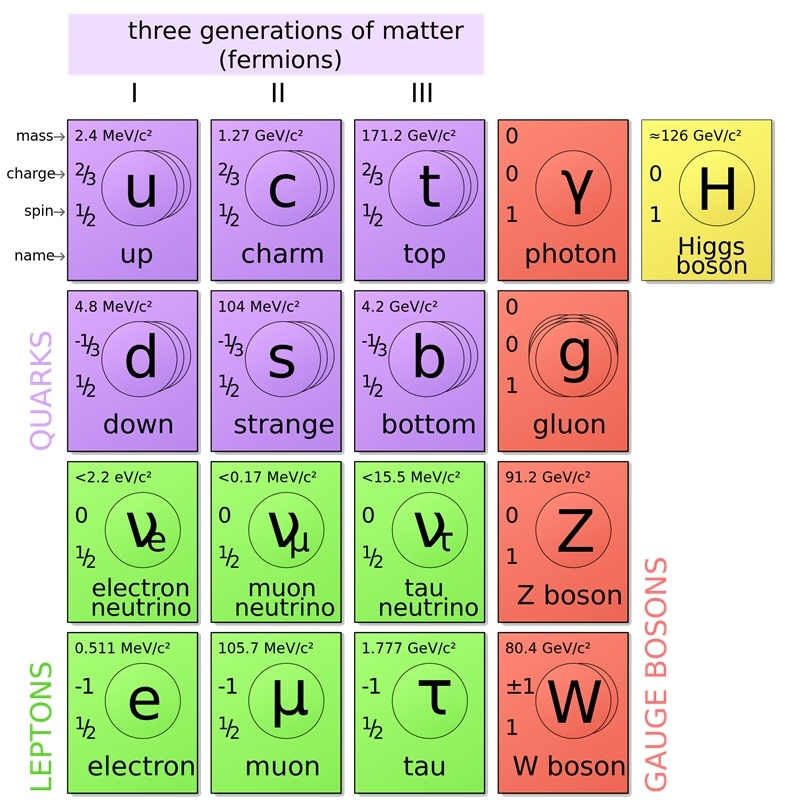
\includegraphics[scale=0.3]{Immagini/SM}
\caption{Particelle elementari del Modello Standard.}
\label{fig:SM}
\end{figure}

Il Modello Standard descrive la materia come composta da due tipi di particelle, entrambi fermioni con spin $\nicefrac{1}{2}$, {\em leptoni} e {\em quark}:

\begin{itemize}
\item i {\em leptoni} hanno carica elettrica intera e quelli conosciuti sono sei, suddivisi in tre generazioni di doppietti con massa crescente. Ogni doppietto è costituito da una particella con carica $Q=-1$ che ha interazioni elettrodeboli, rispettivamente l'elettrone $e$, il muone $\mu$ e il leptone tau $\tau$ nelle tre generazioni. Il doppietto \`e completato da una particella neutra chiamata {\em neutrino}, $\nu_e$, $\nu_{\mu}$ e $\nu_{\tau}$ rispettivamente, che interagisce solo per interazione debole.
\item Analogamente ai leptoni i {\em quark} sono organizzati in doppietti. In questo caso però la carica è frazionaria: la componente superiore del doppietto ha carica $Q=2/3$ ed \`e costituita dai quark $u$, $c$ e $t$ rispettivamente per le tre generazioni. La componente inferiore ha carica $Q=-1/3$ ed \`e costituita dai quark $d$, $s$ e $b$ rispettivamente per le tre generazioni. I quark interagiscono sia elettrodebole che forte e quest'ultima interazione è alla base della formazione di stati legati chiamati adroni, come ad esempio neutrone e protone.
\end{itemize}

Ad ognuna di queste particelle corrisponde una antiparticella che ha i numeri quantici opposti ma stessa massa e spin. Oltre alle antiparticelle il Modello Standard prevede l'esistenza dei {\em bosoni di gauge} e del {\em bosone di Higgs}. I primi sono i mediatori delle interazioni che, a loro volta, derivano dalle simmetrie insite nella teoria:

\begin{itemize}
\item il {\em fotone} \`e responsabile della mediazione dell'interazione elettromagnetica;
\item i {\em bosoni $W^{\pm}$} e $Z$, sono i mediatori dell'interazione debole; un'esempio in cui entra in gioco questa forza è il decadimento $\beta$. Questi bosoni, sono massivi, circa $80\GeVcc$ e $91\GeVcc$ rispettivamente.
\item I {\em gluoni} sono i mediatori dell'interazione forte.
\end{itemize}

Come detto precedentemente la forza gravitazionale non è descritta dal MS, ma risulta essere trascurabile nelle interazione tra particelle, in quanto la sua intensità, paragonata a quella delle altre tre forze, è vari ordini di grandezza inferiore. Nel MS le interazioni sono descritte come manifestazioni di simmetrie di gauge della Lagrangiana. Queste simmetrie non ammettono termini di massa per i bosoni di gauge poiché questo porterebbe alla rottura delle simmetrie stesse. Tuttavia \`e possibile introdurre un meccanismo di rottura spontanea della simmetria, detto {\em di Higgs}, da cui derivano i termini di massa per i bosoni di gauge e un ulteriore bosone scalare massivo, il {\em bosone di Higgs}. Attraverso il meccanismo di Higgs vengono anche introdotti i termini di massa dei fermioni.

{\bf Aggiungere un paragrafetto sulle problematiche del MS (dark matter, teoria efficace a bassa energia etc.). Per questo si costruiscono gli acceleratori ...}

\section{LHC e l'esperimento CMS}
Il {\em Large Hadron Collider} o {\em LHC} è attualmente il più grande acceleratore di particelle mai costruito. Si trova presso il {\em CERN} ({\em European Organization for Nuclear Research}), collocato in un anello sotterraneo di 27~km nella regione di Ginevra (Svizzera). 

LHC \`e un collider adronico in grado di produrre interazioni protone-protone all'energia di $13\TeV$ nel centro di massa. \`E stato progettato con due anelli separati con campo magnetico opposto in modo che i fasci controrotanti possano essere costituiti da particelle con la stessa carica elettrica. Questa caratteristica, oltre ad altre, fa di LHC una macchina di frontiera di ineguagliata complessit\`a che ha richiesto una grande innovazione tecnologica. 

L'accelerazione dei protoni avviene a stadi come schematizzato in~Fig.~\ref{fig:LHC}: i protoni ottenuti da idrogeno gassoso sono inizialmente accelerati da un acceleratore lineare, LINAC2. Successvamente i protoni sono iniettati nel Proton Synchroton Booster (PSB) che aumenta l'energia fino a $1.4\GeV$ e, in seguito, grazie al Proton Synchrotron, raggiungono i $25\GeV$. In queste fasi i protoni vengono raggruppati in pacchetti distanti temporalmente $25\ns$ intervallo che che corrisponde alla frequenza di interazioni di $40\MHz$ a cui LHC opera. 
I protoni vengono infine accelerati fino ad energie di $450\GeV$ nel Super Proton Synchrotron (SPS) prima di essere iniettati nei due anelli di LHC in cui subiscono l'ultima fase di accelerazione fino all'energia di $13\TeV$ prima di farli collidere nei punti in cui sono collocati gli esperimenti.

Il {\em Compact Muon Solenoid} o {\em CMS} è uno dei principali esperimenti di LHC, assieme ad ALICE, ATLAS e LHCb. 

\begin{figure}
\centering
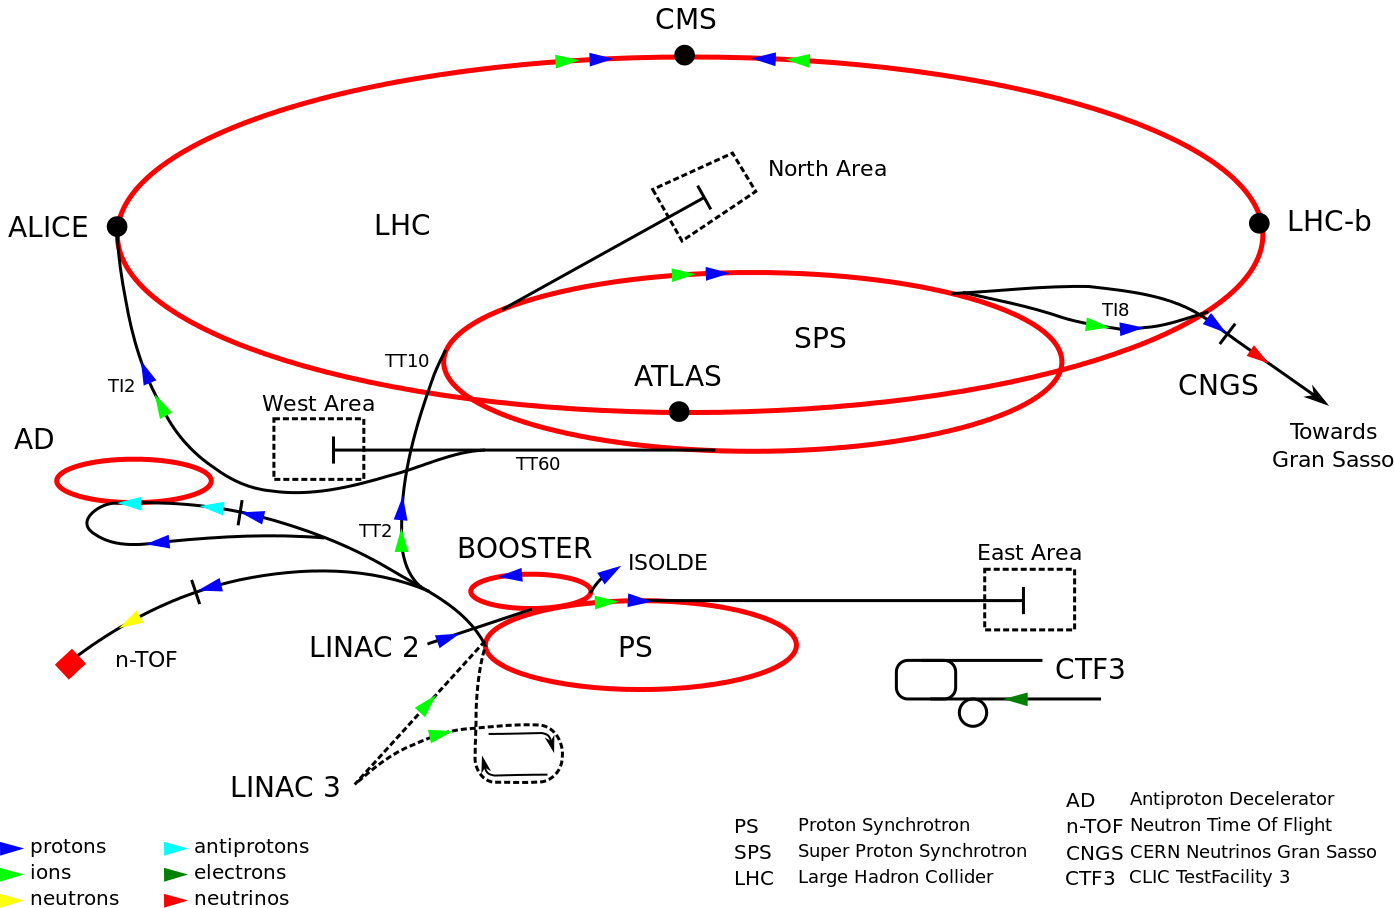
\includegraphics[scale=0.25]{Immagini/LHC}
\caption{Schema di pre-accelerazione e accelerazione di LHC.}
\label{fig:LHC}
\end{figure}

Lo scopo di questi esperimenti è lo studio del MS e la ricerca della materia oscura e di evidenze di nuova fisica, ovvero fenomeni non previsti dal MS stesso. Questi esperimenti sono collocati nei punti in cui i fasci di particelle si incrociano e le interazioni protone-protone prodotte possono essere quindi registrate ed essere analizzate in seguito. Pi\`u nel dettaglio:
\begin{itemize}
\item ALICE (A Large Ion Collider Experiment) \`e un esperimento che studia un stato della materia noto come {\em quark-gluon plasma}, prodotto nelle collisioni di ioni pesanti dal momento che, oltre alle collisioni protone-protone, LHC pu\`o operare come collisionatore ione-ione;
\item CMS (Compact Muon Solenoid) e ATLAS (A Toroidal LHC ApparatuS) sono entrambi progettati con lo scopo di investigare il più ampio spettro di fisica possibile. I due esperimenti hanno gli stessi obbiettivi, ma sono stati costruiti in modo differente al fine di essere indipendenti nello studio dei processi di interazione che avvengono durante le collisioni tra due protoni. Atlas e CMS nel 2012 hanno scoperto il bosone di Higgs~\cite{scopertahiggs}. 
\item LHCb (LHC beauty) \`e un esperimento che studia la fisica degli adroni contenenti il quark b e la violazione di CP (coniugazione di Carica e Parità) nelle interazioni elettrodeboli.
\end{itemize}
Altri esperimenti presenti ad LHC, ma di dimensioni minori sono TOTEM e LHCf:
\begin{itemize}
\item TOTEM (TOTal Elastic and diffractive cross section Measurement), ha come fine lo studio della fisica diffrettiva a piccolo angolo nelle interazioni protone-protone;
\item LHCf (LHC forward) è composto da due rivelatori che sono posizionati a $140$m dal punto di collisione di ATLAS per lo studio delle interazioni calorimetriche dei pioni neutri a grande rapidità e altissima energia, con lo scopo di verificare i modelli di simulazione per meglio modellizzare il comportamento dei raggi cosmici primari nell'interazione con l'atmosfera.
\end{itemize}

In un acceleratore due sono i parametri operativi fondamentali che ne determinano il potenziale di scoperta e la capacit\`a di effettuare accurate misure di fisica: l'energia del centro di massa e la luminosit\`a.

Pi\`u grande l'energia nel centro di massa, maggiore la massa delle particelle che possono essere prodotte e, in generale, a parit\`a di massa, \`e maggiore la sezione d'urto di produzione e quindi il numero di potenziali osservazioni. L'energia nel centro di massa di LHC \`e attualmente $\sqrt{s}=13\TeV$ a cui si \`e arrivati gradualmente: durante il RunI (2010-2012) l'energia del centro di massa \`e stata compresa tra 7 e $8\TeV$ ed \`e stata incrementata al valore attuale per il RunII (2015-2018).  

La struttura non elementare dei protoni, costituiti internamente da partoni (quark e gluoni) che si dividono l'impulso totale, permette di produrre stati di energia intermedia fino al limite cinematico dell'energia del centro di massa e quindi di esplorare un ampio intervallo di energie senza dover modificare i parametri di funzionamento dell'acceleratore. Nella collisione l'interazione effettiva coinvolge solo una coppia di partoni che trasportano una frazione dell'impulso nominale dei due protoni. Questo costituisce un grande vantaggio dei collider adronici rispetto ai collider $\ee$ nell'ambito delle analisi di fisica di scoperta.

%che aumenta la probabilit\`a di produrre  motivo di una così alta energia è spiegato con la necessità di indagare processi fisici i cui effetti sono %maggiormente visibili se si è sopra una certa scala di energia. Un esempio è il Bosone di Higgs scoperto nel 2012, la cui massa è circa $125$ $GeV$.

Un ingrediente fondamentale per raggiungere energie elevate \`e il campo magnetico in cui sono immersi i tubi in cui circolano i fasci che sono inoltre tenuti ad una pressione di vuoto è di $10^{-13}{\mathrm atm}$, per evitare che i protoni interagiscano con le molecole di gas. Il campo magnetico, ortogonale al piano dell'anello, permette ai fasci di rimanere su una traiettoria quasi circolare. In particolare:
\begin{equation}
P[\GeVc] \sim 0.3 \cdot B[{\mathrm T}] \cdot r[\m]
\end{equation}
dove $B$ è il campo magnetico, $r$ il raggio di curvatura e $P$ l'impulso della particella. Dati i parametri di LHC ($r\sim4 \cdot 10^3\m$ e $P=6.5\TeVc$) si ottiene un campo $B$ che in media è pari a $\sim 5.4{\mathrm T}$. Per ottenere un campo di tale intensit\`a è stato necessario sviluppare dipoli magnetici superconduttori, il che ha rappresentato un'importante sfida tecnologica per la progettazione di LHC. Gran parte dell'anello di LHC, infatti, \`e mantentunto a temperature criogeniche di $\sim 2\degrees {\mathrm K}$ grazie ad un complesso sistema di raffreddamento.

{\bf correggere definizione luminosit\`a}

La {\em luminosit\`a} \`e proporzionale al numero di interazioni che l'acceleratore pu\`o fornire agli esperimenti ed \`e una grandezza fondamentale per stimare la capacit\`a dell'acceleratore di produrre eventi con piccola sezione d'urto e, quindi, la possibilit\`a degli esperimenti di osservarli. Al fine di ottenere risultati con un'ampia statistica ed una buona precisione è importante per un acceleratore avere una alta luminosità istantanea, un parametro che corrisponde al numero di collisioni prodotte per unità di area e tempo e può essere espressa in funzione del rate R di particelle {\bf(che cazzo vor di'?????)} e della sezione d'urto $\sigma$ 
\begin{equation}
L=\frac{R}{\sigma}
\end{equation}
Un altro modo di esprimere la luminosità è metterla in funzione delle variabili che caratterizzano il fascio:
\begin{equation}
L = f \frac{N_1 N_2}{4 \pi \sigma_x \sigma_y}
\end{equation}
con $N_1$ $N_2$ numerodi protoni per pacchetto, $f$ frequenza collisioni e $4\pi \sigma_x \sigma_y =A$ area efficace. Si parla invece di {\em luminosità integrata} $L_{int}=\int L dt$ per ottenere la relazione tra numero di eventi relativi a un certo processo e la sezione d'urto $\sigma$ del processo stesso:
\begin{equation}
N=\sigma L_{int}.
\end{equation}

\section{HL-LHC}
Il progetto di upgrade HL-LHC, formalmente approvato nel Giugno 2016 dal CERN, permetter\`a di ampliare il campo di indagine di fenomeni fisici rari all'interno del MS ed anche di ricercare processi di nuova fisica BSM (Beyond Standard Model). Questa fase di alta luminosità permetterà a CMS di raggiungere precisioni dell'ordine del per cento sulle misure di accoppiamento del bosone di Higgs e la prima osservazione diretta di vertici trilineari del bosone di Higgs. 
I processi deboli di scattering di bosoni vettori sono profondamente legati alla rottura della simmetria elettro bedole e dal punto di vista della misura sono una sfida, in quanto le sezioni d'urto sono piccole e i fondi irriducibili sono dominanti. 

L'aumento di luminosità ad LHC permetterà lo studio di questi canali, per far ciò  l'upgrade di LHC sarà accompagnato da un programma di adeguamento dell'esperimento CMS, al fine di mantenere alte le prestazioni del rivelatore (efficienza, risoluzione,reiezione di processi di fondo...) nonostante l'aumento di radiazione e le più difficili condizioni operative, come ad esempio pile-up più frequente.
In figura \ref{HL-LHC} è mostrato un prospetto della scaletta dei tempi di LHC dal 2015 in poi. Il Run 2 continuerà fino alla fine del 2018, quando inizierà il Long Shutdown 2 (LS2) e dopo cui si avrà la fase di Run 3.  Entro il 2022 si stima sarà raccolta una luminosità integrata di circa $300 fb^{-1}$. 
Durante il Long Shutdown 3 (LS3), programmata dal 2022 fino alla metà del 2024, saranno eseguiti gli aggiornamenti principali di LHC e degli esperimenti per la fase di alta luminosità.

\subsection{Obiettivi}
\begin{figure}
\centering
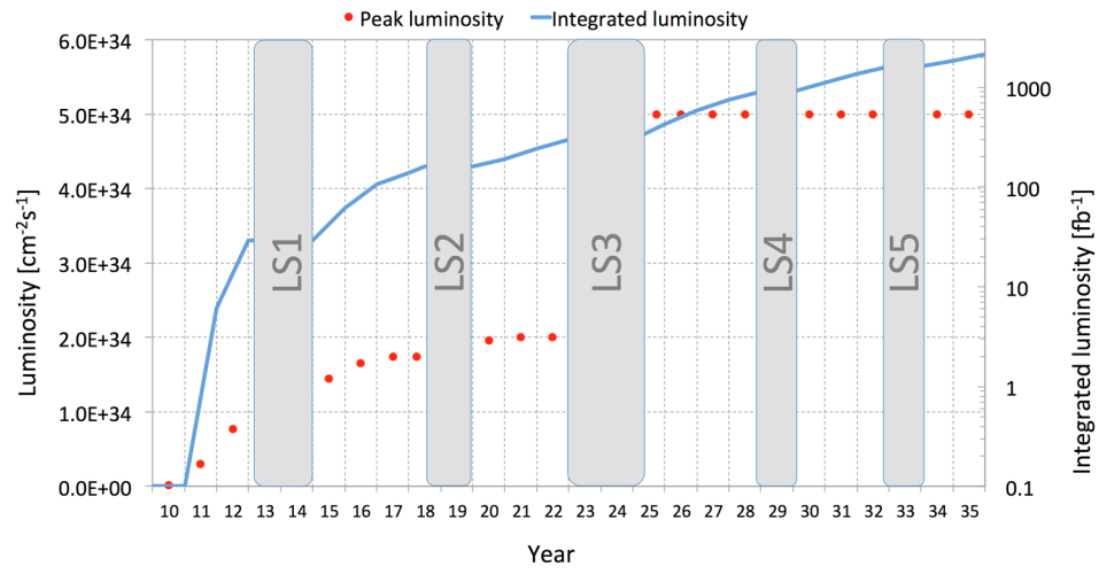
\includegraphics[scale=.35]{Immagini/HL-LHC}
\caption{Projected LHC performance through 2035, showing preliminary dates for long shut downs of LHC and projected luminosities.reference LHCC P 008}
\label{HL-LHC}
\end{figure}

L'idea di aumentare la luminosità di LHC oltre quella decisa nel progetto originale è antecedente alla messa in opera del progetto. Eventuali modifiche importanti alla macchina e agli esperimenti possono essere eseguite solo con lunghi periodi di shut down in cui è possibile accedere al tunnel e alle caverne. Per questo motivo è stato deciso un piano temporale che intervalli periodi di presa dati (Run I, Run II etc.) e periodi in cui si ha uno spegnimento completo per lunghi periodi (LS1, LS2, LS3). In figura \ref{HL-LHC} è possibile vedere la suddivisione temporale tra periodi di presa dati e periodi di spegnimento.
Run I è stato il periodo di presa dati dal 2011 al 2012. Nel primo periodo di stop LS1 LHC è stato modificato al fine di raggiungere energie  nel centro di massa di 13 TeV, per poi arrivare gradualmente a 14 TeV. In questo momento siamo alla fine del Run II, e nell'esperimento CMS si  hanno una media di 25 interazioni per bunch, ciò vuol dire 25 vertici da ricostruire ogni 25 ns. Attraverso modifiche  e miglioramenti apportati nel LS1 e LS2 verrà aumentata la luminosità, questa parte del processo per l'esperimento CMS va sotto il nome di fase-I. Durante il periodo LS3  saranno invece sostituite vari parti degli esperimenti, che a causa del danneggiamento da radiazione saranno deteriorati e nello contemporaneamente verranno sostituiti i quadrupoli di fuocheggiamento con nuovi modelli capaci di incrementare la luminosità. 
Il periodo che seguirà LS3 sarà chiamato fase II o HL-LHC (High Luminosity LHC). Nello scenario prefissato la lumiosità istantanea sarà di $5 \cdot 10 34 cm^{-2} s^{-1}$ con picchi di $2 \cdot 10 35 cm^{-2} s^{-1}$, in questo modo gli esperimenti saranno in grado di raccogliere una maggiore statistica con una luminosità di $300 fb^{-1}$ ogni anno per 10 anni(250 o 300)?????%at 5 × 10 34 cm − 2 s − 1 from a potential peak value of 2 × 10 35 cm − 2 s − 1 at the beginning of fills,
%and to deliver 250 fb − 1 per year for a further 10 years of operation. Under these conditions
In queste condizioni ci sarà una maggiore probabilità di sovrapposizione di interazioni (Pile Up), questa sarà la grande sfida, insieme alla gestione degli effetti di degradazione in cui incorreranno i rivelatori a seguito delle maggiori dosi di radiazione assorbita. Sempre nella figura \ref{HL-LHC} è possibile vedere le proiezioni di luminosità di picco e luminosità integrata.
 
%The high luminosity period that follows LS3 with the upgraded LHC is referred to here as HL-LHC or Phase-II. The proposed operating scenario is to level the instantaneous luminosity
%at 5 × 10 34 cm − 2 s − 1 from a potential peak value of 2 × 10 35 cm − 2 s − 1 at the beginning of fills,
%and to deliver 250 fb − 1 per year for a further 10 years of operation. Under these conditions the event PU will rise substantially to become a major challenge for the experiments, and the performance degradation due to integrated radiation dose will need to be addressed. This Technical Proposal presents the CMS upgrade program for Phase-II. The schedule of beam operations and long shutdowns, together with projections of the peak and integrated luminosities, is shown in Fig. 1.9, and is, of course, subject to change.

\section{Esperimento CMS}
CMS è un esperimento ad ampio spettro che opera ad LHC, è installato un centinaio di metri sotto terra CMS nei pressi del paese Cessy, in Francia, tra il lago di Ginevra e il complesso dei monti Jura. Essendo ad ampio spettro i suoi rivelatori sono in grado di distinguere un gran numero di particelle $e$, $\mu$, $\tau$, $\gamma$ etc...
L'obiettivo principe di LHC è quella di indagare la natura della rottura spontanea della simmetria elettrodebole alla base di cui sta il meccanismo di Higgs. Lo studio sperimentale del meccanismo di Higgs consente inoltre di verificare la consistenza del Modello Standard a scale di energia dei TeV. Inoltre c'è la speranza di nuove scoperte che offrano indicazioni su teorie oltre al Modello Standard, come ad esempio Supersimmetrie o Extra Dimension.
Ad LHC vengono utilizzati anche fasci di ioni pesanti, che hanno energie 30 volte superiori ai precedenti acceleratori, permettendo così uno studio approfondito della QCD in condizioni estreme di temperatura, densità e frazioni di momento partonico. Con la luminosità ed energia nel centro di massa raggiungibili ad LHC un ampio spettro di fisica diventa accessibile, questo però vincola i vari esperimenti, compreso CMS a richieste stringenti sulle prestazioni e quindi sulla progettazione e messa in opera.
Con un'energia nel centro di massa di 14 TeV la sezione d'urto protone-protone è circa 100 mb, data la  luminosità questo porta a circa $10^9$ eventi al secondo, che grazie al processo di selezione online viene abbassato fino a 100 eventi al secondo, i quali vengono poi memorizzati per una successiva analisi. 
Ogni 25 ns vi è una nuova collisione tra bunch di particelle che con le sue circa 20 collisioni produce un alto numero di particelle che dovranno essere rivelate con l'attenzione a distinguerle le une dalle altre. Questo richiede un'alta segmentazione del rivelatore e una buona risoluzione temporale , al fine di evitare effetti di pile-up. Il tutto cercando di ridurre il più possibile i volumi.
Inoltre dato l'alto flusso di particelle il rivelatore e l'elettronica di lettura devono essere in grado di resistere ad alti livelli di radiazione. Tutti questi motivi hanno  portato alla necessità di alti requisiti per il buon funzionamento dell'esperimento:
\begin{itemize}
\item Buona capacità di identificare i muoni e ottima risoluzione degli impulsi su ampio angolo.
\item Alta efficienza del tracciatore e buona risoluzione dei momenti di particelle cariche.
\item Buona risoluzione nella misura dell'energia elettromagnetica, copertura maggiore possibile di tutto l'angolo solido e ottima capacità di isolamento di fotoni e leptoni.
\item Buona risoluzione dell'energia trasversa mancante (MET) e calorimetri adronici con coperture ampia dell'angolo solido e buona segmentazione.
\end{itemize}

Il sistema di coordinate adottato da CMS è tale che l'origine corrisponde al punto di collisione dei due fasci con asse y verticale orientato verso l'alto e asse x in direzione radiale verso il centro di LHC. L'angolo azimutale $\phi$ è misurato a partire dall'asse x e giace sul piano x-y e la coordinata radiale su questo piano è $r$. L'angolo polare $\theta$ è misurato dall'asse z. 

Per lo studio dei processi è utile introdurre anche grandezze invarianti per trasformazioni di Lorentz come $\Delta y$ e $\Delta \eta$, dove y indica la rapidità e $\eta$ la pseudorapidità:
\begin{equation}
y= \dfrac{1}{2} ln\Big( \dfrac{E+p_z}{E-p_z}\Big)
\end{equation}

\begin{equation}
\eta = - ln \Big( tg\frac{\theta}{2}\Big)
\end{equation}
Infine la differenza nel bilancio dell'energia misurata sul piano trasverso è indicata come $E_T^{miss}$.


\subsection{Il rivelatore CMS}
CMS è un esperimento a simmetria cilindrica, ha un diametro di 15 m ed è lungo 21.6 m, per un peso complessivo di circa 12500 tonnellate. Lo scopo dell'esperimento è studiare una vasta gamma di processi fisici delle interazioni protone-protone, figura \ref{CMS}. 
\begin{figure}
\centering
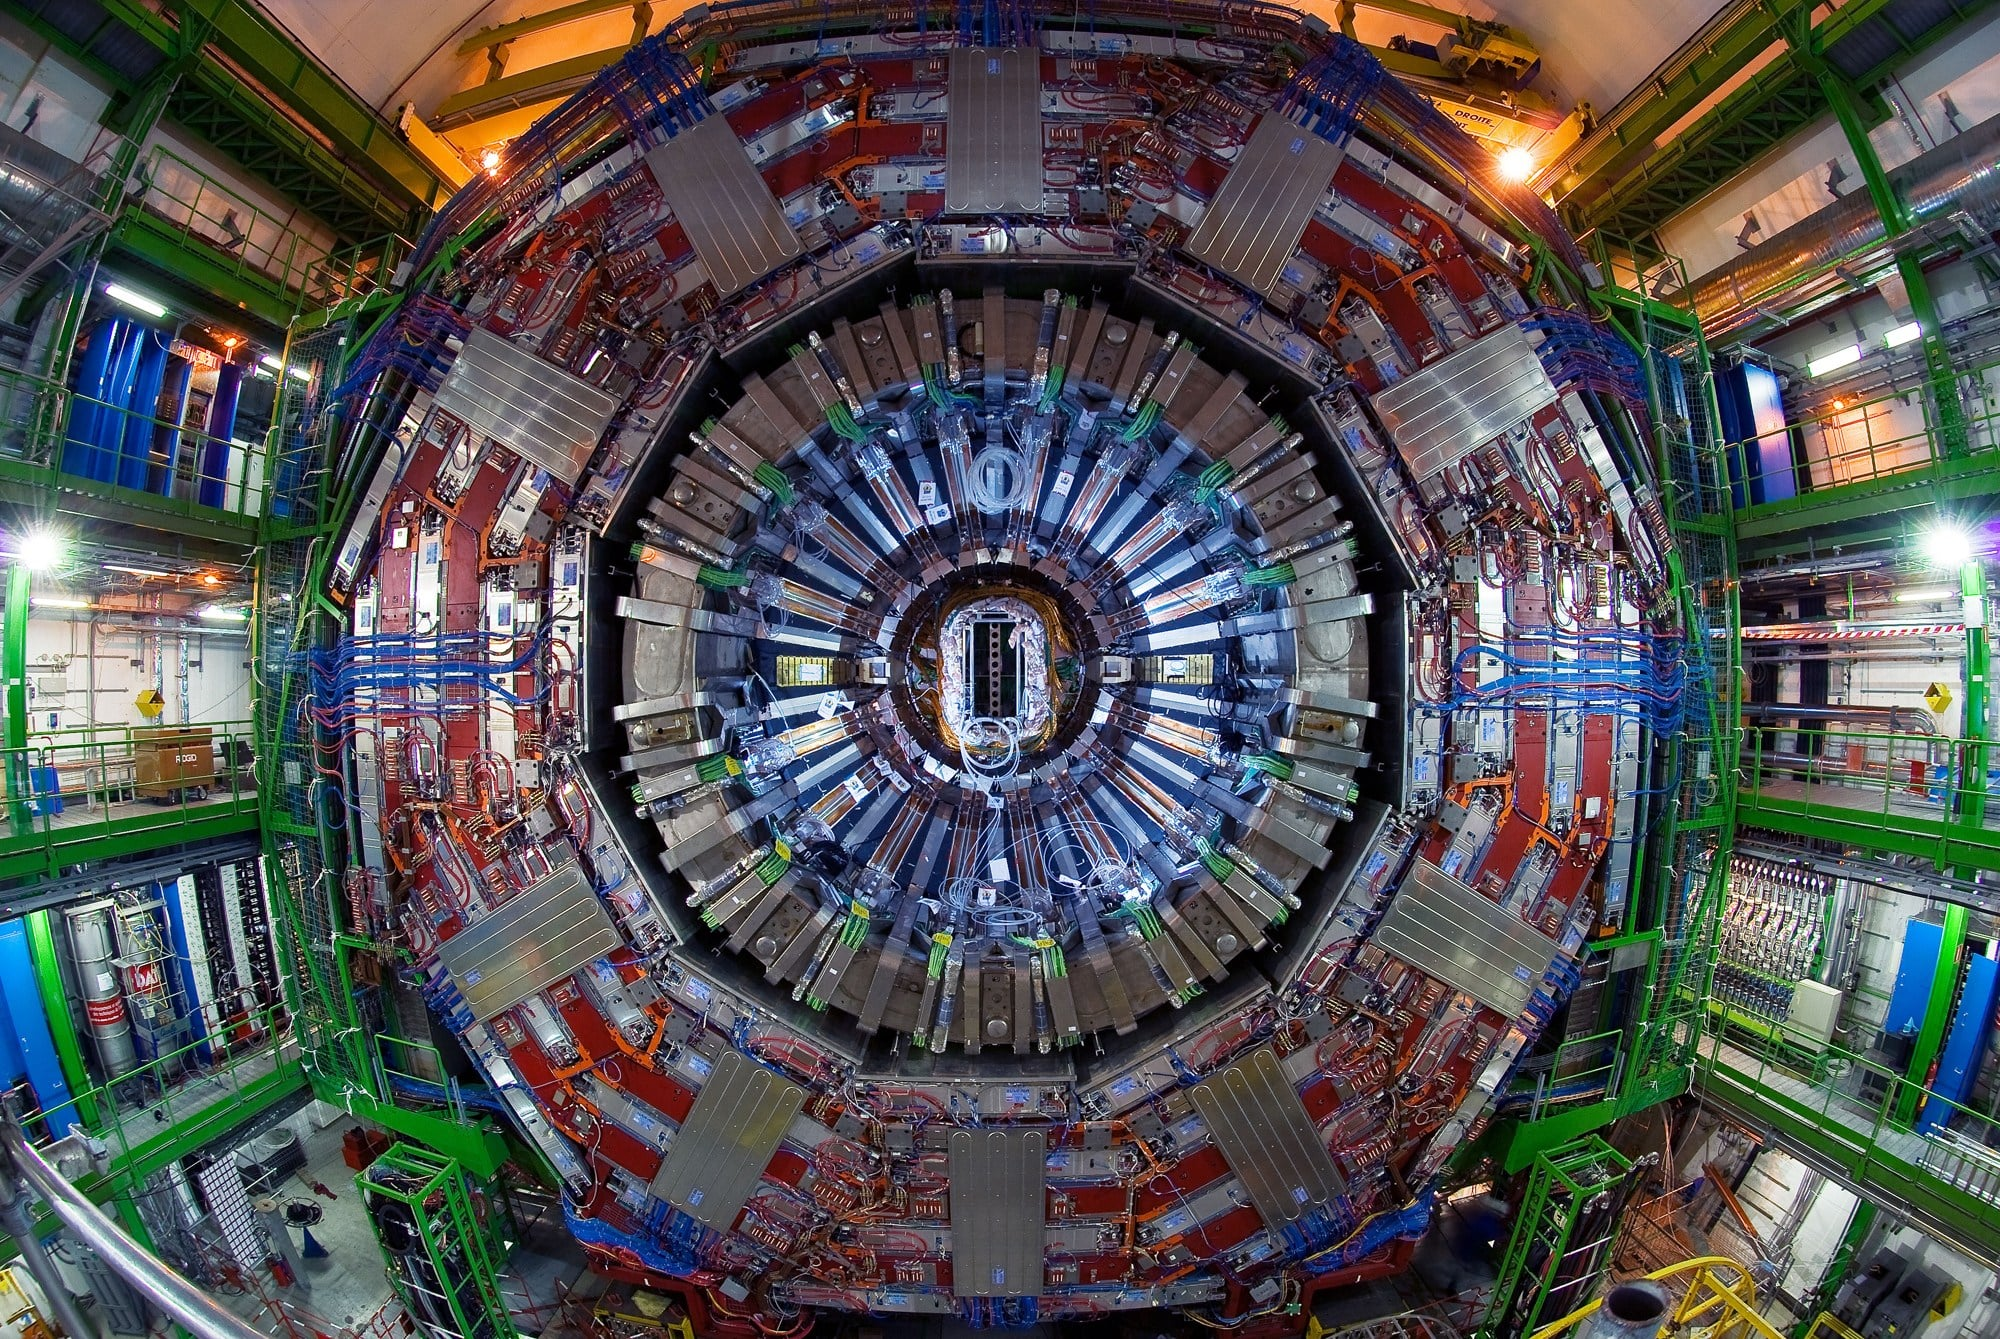
\includegraphics[scale=.2]{Immagini/CMS}
\caption{Vista frontale di CMS durante l'installazione del tracciatore.}
\label{CMS}
\end{figure}
Per questo motivo è composto da diversi tipi di rivelatori, vedi figura \ref{CMSbis}, disposti in modo concentrico rispetto al punto di collisione dei due fasci:
\begin{itemize}
\item \textbf{Tracciatore}: collocato nella parte più interna è in grado di ricostruire la traiettoria delle particelle cariche  nella zona r $< 1.2$ m e $\mid\eta\mid$ $< 2.5$ individuando anche
eventuali vertici secondari. È suddiviso in due sottorivelatori: un rivelatore di vertice a pixel di silicio e un rivelatore a microstrip di silicio.

\item \textbf{Calorimetro elettromagnetico} (ECAL): è un calorimetro omogeneo composto da cristalli di tungstato di piombo (PbW$\mathrm{O_4}$), collocato nella regione 1.2 m $<$ $\mid$r$\mid$ $< 1.8$ m ed $\mid\eta\mid < 3$ misura l'energia di elettroni e fotoni, oltre che la traiettoria.

\item \textbf{Calorimetro adronico} (HCAL): posto nella regione con 1.8 m $<$ $\mid$r$\mid$ $< 2.9$ m ed $\mid\eta\mid$ $<$ 5, fornisce informazioni sull’energia e traiettoria delle particelle
adroniche. Il calorimetro utilizza strati di ottone alternati a strati di scintillatore plastico ed è suddiviso in quattro parti: HB (Barrel Hadronic Calorimeter) e HE (Endcap Hadronic Calorimeter) situati all’interno del magnete nella zona del barrel e dell’endcap, HO (Outer Hadronic Calorimeter) situato all'esterno del magnete e il HF (Forward Hadronic Calorimeter) anch'esso esterno al magnete e posto nella regione in avanti.

\item \textbf{Magnete superconduttore solenoidale}: posto nella regione 2.9 m $<$ r $< 3.8$ m, genera un campo magnetico uniforme di 3.8 T lungo la direzione dei fasci. Ciò permette di curvare la traiettoria delle particelle cariche, specialmente dei muoni, consentendo così di misurarne l'impulso trasverso. Il flusso del campo magnetico si richiude su un giogo di
ferro con diametro circa 14 m e lunghezza 21.6 m. In questa zona è presente una campo residuo di 1.8 T in direzione opposta a quello interno.

\item \textbf{Camere a muoni}: sono poste tra i vari strati del giogo di ritorno del campo magnetico, nella regione 4 m $<$ r $<$ 7.4 m e $\mid\eta\mid$ $<$ 2.4 e come dice il nome hanno il compito di rivelare i muoni. Queste camere a muoni sono di tre tipi, camere a deriva (DT) nel barrel, camere a strisce catodiche (CSC) nelle regioni estreme che chiudono il rivelatore, dette endcap, e camere a piastra resistiva (RPC).

\end{itemize}
%La parte centrale di CMS è racchiusa in un solenoide superconduttivo lungo 13 metri e con un diametro di 6, capace di generare un campo di $3.8 T$, questo consente  di curvare abbastanza la traiettoria di tutte le particelle cariche e specialmente dei muoni, consentendo così di misurarne l'impulso trasverso. Il campo magnetico del solenoide si richiude su un giogo di ritorno in ferro, inframezzato al ferro del giogo sono posizionati i rivelatori di muoni. Ogni rivelatore di muoni consta di vari strati di Drift Tubes in allumnio (DT) sulla superficie cilindrica e cathode strip chamber (CSC) nelle regioni estreme che chiudono il rivelatore, dette endcap, a questi si aggiungono le resistive plate chamber (RPC). 
%Nella parte interna del magnete è contenuto il tracciatore e i calorimetri. Per quanto riguarda il tracciatore la parte più interna è composta da 3 piani di rivelatori a pixel in  silicio, più esternamente sono stati installati 10 piani di rivelatori a microstrip di silicio. 
%Sempre internamente al solenoide sono posti intorno al tracciatore i calorimetri elettomagnetici (ECAL) utilizza cristalli di tungstato di piombo ($PbWO_4$) con copertura in pseudorapidità fino a  $|\eta |< 3.0$. La luce di scintillazione viene letta a fotodiodi a valanga di silicio (APDs) e fototriodi a vuoto (VPTs) nelle regioni di endcup, dove il campo magnetico è basso. 
\begin{figure}
\centering
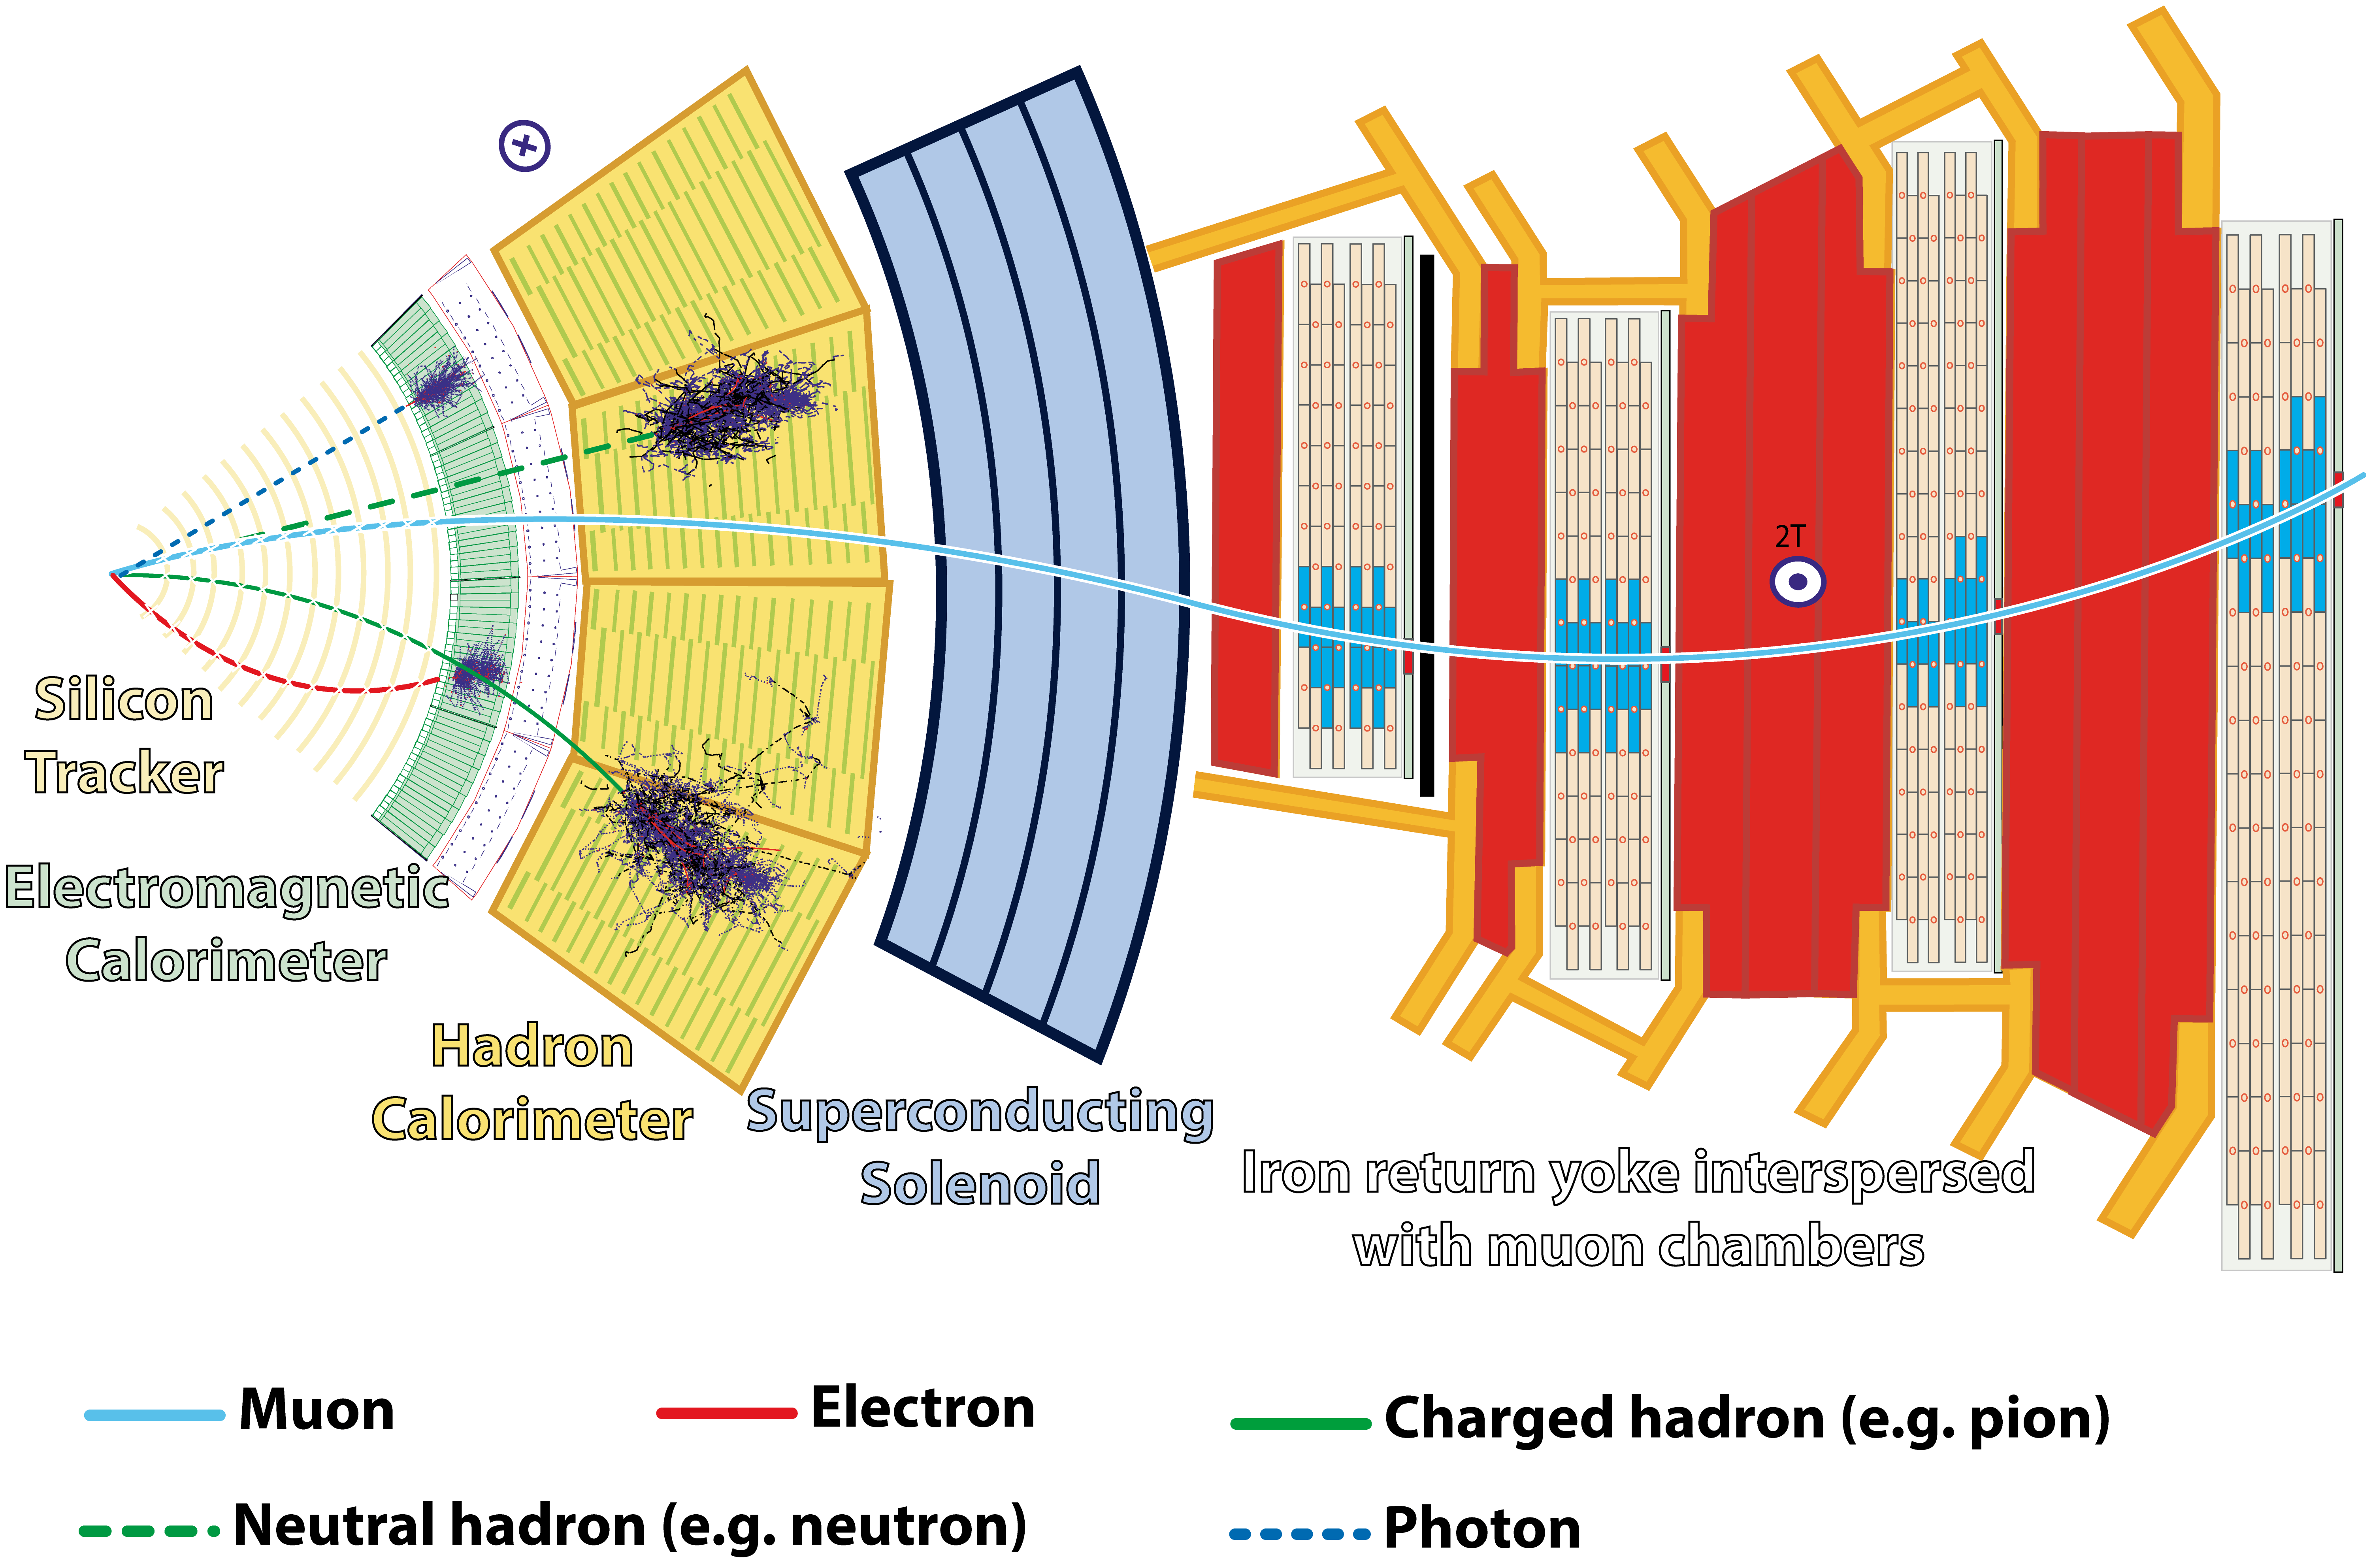
\includegraphics[scale=0.8]{Immagini/CMSbis}
\caption{Spaccato di CMS e risposta ai vari tipi di particella.}
\label{CMSbis}
\end{figure}

Questa struttura rispecchia la necessità di ricostruire con precisione gli eventi originati dalla collisione di particelle, che avvengono in rapida successione. CMS come anche gli altri esperimenti, può essere paragonato ad una gigantesca macchina fotografica che registra 40 milioni di foto al secondo (digitalizzando l'informazione di decine di milioni di sensori). 
La struttura a strati consente di avere rivelatori diversi in ogni strato, di cui i più interni sono meno densi, mentre i più esterni sono più densi. Questo perché il tracciatore non deve alterare l'energia delle particelle che poi sarà misurata nei calorimetri e per facilitare la ricostruzione delle tracce è importante evitare fenomeni di multiple scattering.

Le particelle che gli scienziati cercano di riprodurre nelle collisioni protone-protone hanno vite medie molto brevi, e decadono rapidamente in particelle più leggere. Dopo un processo di hard-scattering migliaia di queste particelle leggere sono generate elettroni, muoni, fotoni, ma anche protoni, neutroni etc. Tutte queste particelle attraversano i vari strati di cui è composto il rivelatore. 
Le informazioni raccolte vengono utilizzate per ricostruire l'evento di interazione, per  dedurre l'esistenza di nuove particelle.


Le traiettorie delle particelle cariche sono piegate dal campo magnetico, e il loro raggio di curvatura è utilizzata per calcolare il loro impulso: maggiore è la loro energia cinetica, minore è la curvatura. Un'altra componente importante di un rivelatore sono i calorimetri per misurare l'energia delle particelle (sia cariche che non). 
I calorimetri devono essere abbastanza grandi per assorbire anche le particelle più energetiche. Questi motivi fanno sì che gli esperimenti ad LHC siano così grandi. I rivelatori sono costruiti in modo il più possibile ermetico per raccogliere tutti i prodotti delle interazioni e poter ricostruire gli eventi. 
Combinando le informazioni di ogni strato del rivelatore è possibile determinare il tipo di particella che ha lasciato una data traccia.

Particelle cariche come elettroni, protoni e muoni, lasciano tracce ionizzando il materiale attraversato. Gli elettroni sono molto leggeri e perciò perdono energia velocemente, mentre i protoni penetrano più in profondità negli strati del rivelatore. I fotoni essendo neutri non rilasciano segnali nel tracciatore, ma nei calorimetri sono convertiti in elettroni e positroni e così ne viene misurata l'energia. 
L'energia dei neutroni viene invece misurata indirettamente, trasferiscono l'energia ai protoni, che poi sono misurati. I muoni insieme ai neutrini (che non vengono rivelati) sono i soli a raggiungere gli strati più esterni.


\begin{figure}
\centering
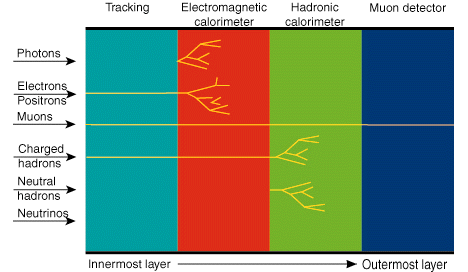
\includegraphics[scale=0.7]{Immagini/CMSinterazione}
\caption{Spaccato di CMS e risposta ai vari tipi di particella.}
\label{CMSinterazione}
\end{figure}

Ogni parte del rivelatore è connessa ad un sistema di lettura elettronico attraverso migliaia di cavi. Ogni volta che un segnale è raccolto, il sistema registra la sua posizione e l'istante in cui è stato raccolto, se il sistema di trigger decide che l'evento che ha generato Se tale segnale è di interesse, allora l'informazione è letta e portata all'esterno del rivelatore per essere utilizzata nelle analisi offline.
Ci sono differenti criteri per selezionare un evento potenzialmente di interesse, in questo modo la mole enorme di eventi registrati in un secondo viene ridotta a poche centinaia, che poi verranno analizzate in dettaglio.


\subsection{Tracciatore}
Il tracciatore al silicio  è il rivelatore più vicino al punto dove collidono i due fasci. 
\begin{figure}
\centering
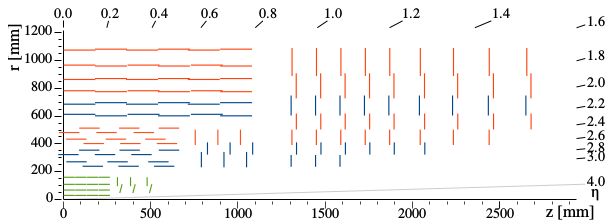
\includegraphics[scale=0.4]{Immagini/CMStracker2}
\caption{Schema di un quarto del tracciatore di CMS visto nel piano $rz$. Il rivelatore a pixel è rappresentato in verde, mentre i moduli a strip singoli e doppi sono in rispettivamente in rosso e blu.}
\label{CMStracker}
\end{figure}
Lo scopo è ricostruire , con la maggior precisione possibile, le traiettorie delle particelle cariche, identificando vertici primari e secondari. La composizione interna del tracciatore è mostrata in figura \ref{CMStracker}. Il raggio esterno è circa 110 cm e la lunghezza totale circa 540 cm.

Nella zona centrale (barrel) e più interna vi è il rivelatore di vertice a pixel, con tre strati distanti 4, 7 e 11 cm dall'asse dei fasci. La dimensione dei pixel è $100x150$ $\mu m^2$. Più esternamente ci sono rivelatori a microstrip tra 20 e 110 cm. Le parti laterali, dette endcap, sono invece costituite da 2 piani a pixel e 9 a microstrip. La parte di microstrip è divisa in due parti Inner Barrel e Outer Barrel, figura \ref{CMStracker}:
\begin{itemize}
\item Tracker Inner Barrel (TIB), costituito di 4 cilindri posti intorno ai piani a pixel.
\item Tracker Inner Discs (TID), 3 dischi posti nella parte interna di endcup.
\item Tracker Outer Barrel (TOB), 6 cilindri che formano la parte esterna del barrel.
\item Tracker EndCaps (TEC), 9 dischi che completano la parte più esterna di endcup.
\end{itemize}

%The Tracker will suffer significant radiation damage by LS3 and must be completely re-
%placed for Phase-II. To maintain adequate track reconstruction performance at the much higher
%PU pileup levels of the HL-LHC, the granularity of both the outer tracker and the pixel systems will
%be increased by roughly a factor 4. In the outer tracker, this will be achieved by shortening the
%lengths of silicon sensor strips relative to those in the current detector, without changing the
%pitch very significantly. A number of design improvements will lead to a much lighter Outer
%Tracker providing significantly improved p T resolution and a lower rate of γ-conversions com-
%pared to the present detector. In addition, the module design will be capable of providing track-stub information to the L1 trigger at 40 MHz for tracks with p T ≥ 2 GeV . This will en-
%sure powerful background rejection at the earliest stage of the event selection. The pixel system
%will implement smaller pixels and thinner sensors for improved impact parameter resolution
%and better two-track separation. This will improve b-tagging as well as τ-hadronic decay and
%track reconstruction efficiencies within boosted jets. With up to 10 additional pixel disks in
%each of the forward regions the system coverage will be extended to close to | η | = 4, to better
%match the range of coverage of the calorimetry.
\subsection{Tracciatore di fase II}

Al fine di mantenere o migliorare le prestazioni di CMS nelle condizioni di alto pile-up e alto danneggiamento da radiazioni, nella fase  di HL-LHC, l'intero sistema di tracciatura delle particelle dovrà essere sostituito con nuovi rivelatori capaci di sostenere livelli di radiazione maggiori e con maggiori funzionalità.
\begin{figure}
\centering
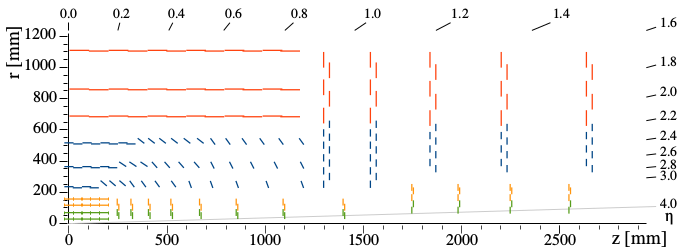
\includegraphics[scale=0.4]{Immagini/TrackerPhaseII}
\caption{Schema rappresentante un quarto del tracciatore. La parte esterna del tracciatore è in blu (moduli PS) e rosso (moduli 2S). La parte del tracciatore a pixel, con l'estensione in avanti è rappresentata in verde e giallo.}
\label{TrackerPhaseII}
\end{figure}

Le limitazioni dell'attuale tracciatore ne impediscono l'utilizzo nella fase di alta luminosità. I principali requisiti per il nuovo rivelatore sono i seguenti, figura \ref{TrackerPhaseII}:

\begin{itemize}
\item \textbf{Tolleranza alla radiazione}: Si prevede che il nuovo tracciatore dovrà operare, mantenendo alta l'efficienza, fino ad una luminosità integrata di 3000 $\mathrm{fb^{-1}}$. Inoltre per la parte esterna del tracciatore non si prevedono interventi di manutenzione, mentre per la parte di tracciatore a pixel sono sotto studio opzioni che consentano di operare sostituzioni nella zona più interna. 
\end{itemize}

\[
\begin{array}{lccc}

\toprule
\mathrm{Regione} & \mathrm{Fluenza \quad massima} [n_{eq}/cm^2] & r [mm] & z[mm]  \\

\midrule

\mathrm{IT \quad barrel \quad layer 1} & 2.3\times10^{16} & 28 & 0\\

\mathrm{IT\quad barrel\quad layer 2} & 5.0\times10^{15} & 69 & 0\\

\mathrm{IT\quad barrel\quad layer 4} & 1.5\times10^{15} & 156 & 89\\

\mathrm{IT\quad forward,\quad ring 1} & 1.0\times10^{16} & 51 & 252\\

\mathrm{IT\quad service\quad cylinder} & 9.6\times10^{14} & 170 & 260\\

\bottomrule
\end{array}
\]

\begin{itemize}
\item \textbf{Alta risoluzione e un migliore sistema di separazione delle tracce}: l'attuale tracciatore ha prestazioni peggiori nel tracciare jet di alta energia, a causa della sovrapposizione di più hit nel rivelatore a pixel. Al fine di sfruttare al meglio la maggiore statistica che ci sarà con HL-LHC, è necessario migliorare la capacità nel distinguere due tracce molto vicine. 
Allo stesso modo  per assicurare alta efficienza, nonostante un maggiore pile-up, è necessaria una maggiore densità di canali di lettura. Come riferimento si stima che la media di pile-up per ogni bunch crossing sarà di circa 140, a fronte dei 40 attuali.

\item \textbf{Riduzione di materiale}: un fattore importante che limita l'attuale risoluzione  è la quantità di materiale che le particelle attraversano. Questo è responsabile di perdita di energia e scattering multipli, i quali causano un peggioramento nelle prestazioni dei calorimetri e nella precisione di ricostruzione dell'evento.

\item \textbf{Sistema di riconoscimento delle tracce affidabile e veloce}: maggiore pile-up significa complicazioni nella ricostruzione delle tracce e tempi più lunghi. La velocità nella ricostruzione è essenziale per la funzionalità del trigger di alto livello (High -Level Trigger). 

\item \textbf{Compatibilità con il nuovo trigger L1}: La selezione degli eventi nella nuova fase ad alta luminosità è una sfida importante, non solo per l'alto numero di particele e quindi tracce, ma anche perché l'alto numero di pile-up rende inefficienti gli algoritmi di selezione degli eventi. Per questo motivo parte del processo di ricostruzione, che attualmente è svolto ad alto livello, sarà spostato in L1il cui rate massimo raggiungerà i 750 kHz.

\item \textbf{Estensione della regione di accettanza delle tracce}: altri benefici per CMS possono essere ottenuti ampliando la copertura della regione in avanti da parte del tracciatore e dei calorimetri.

 
\end{itemize}


\subsection{Tracciatore interno}
La parte interna del tracciatore sarà dotata di moduli a pixel. Come già evidenziato, nella fase ad alta luminosità il punto cruciale per la progettazione sarà la tolleranza alla radiazione di di sensori e elettronica di lettura, come anche la parte di gestione dei dati e l'aumento di frequenza di lavoro per il trigger. 
I candidati per i sensori che  rispettano le richieste su risoluzione, separazione delle tracce e occupazione sono sensori di silicio, di spessore 100-150 $\mu$m, con pixel di 25 $\times$ 100 $\mu m^2$ o 50 $\times$ 50 $\mu m^2$. 
Di conseguenza il chip di lettura dovrà avere celle di piccola dimensione con basse soglie. Lo sviluppo di questo nuovo chip è portato avanti dalla collaborazione RD53 che vede insieme ATLAS e CMS, il progetto prevede un chip con celle di dimensione 2500 $\mu m^2$  in tecnologia CMOS a 65 nm. 
Tale configurazione dovrebbe consentire una migliore resistenza al danneggiamento da radiazione.

\subsubsection{Sensori}
\begin{figure}
\centering
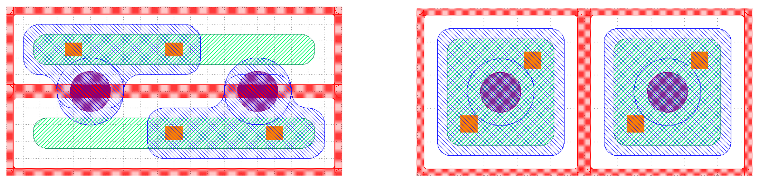
\includegraphics[scale=0.35]{Immagini/Sensors}
\caption{Schema di due celle adiacenti con dimensioni $\mathrm{25 \times 100 \mu m^2}$ (sinistra) e $\mathrm{50 \times 50\mu m^2}$ (destra). Gli impianti n+ sono riportati in verde, in blu le metallizzazioni, in rosso le aree di p-stop , i contatti in arancione e in viola i le piazzole per i bump bond.}
\label{Sensors}
\end{figure}
L'ambiente in cui saranno immersi i sensori nella fase di alta luminosità sarà estremo sia in termini di luminosità integrata che istantanea. 
I sensori saranno esposti ad una fluenza di  $2.3 \times 10^{16} \mathrm{n_{eq}/cm^2}$ negli strati più interni del tracciatore con una luminosità integrata di 3000$\mathrm{fb^{-1}}$. La dose equivalente è circa 12 MGy (1.2 Grad). 
Date queste condizioni si è preferito optare per sensori il più sottili possibile, dato che il vantaggio di raccogliere più carica con sensori più spessi viene annullato dal peggioramento delle prestazioni dovuto all'aumento di difetti nel silicio, a causa dell'alto irraggiamento. 
Lo spessore attivo del sensore, nel caso pixel planare sarà tra i 100 e 150 $\mu$m ( nella fase-0 e fase-1 lo spessore dei pixel era tra i 270  e i 285 $\mu$m). 
Il test di questi sensori insieme ai chip di lettura dimostrerà la fattibilità di utilizzo di questo tipo di sensore in ambienti con alti livelli di radiazione, o se saranno necessarie modifiche. 
Rispetto al tracciatore di CMS di fase-1 l'area dei pixel sarà ridotta di un fattore 6. Le due possibilità prese in considerazione sono $\mathrm{25 \times 100 \mu m^2}$ e  $\mathrm{50 \times 50 \mu m^2}$. 
Nel processo di valutazione dei vari progetti per i pixel particolare rilevanza hanno i seguenti punti:
\begin{itemize}
\item \textbf{Metodo di contro polarizzazione}Schema di polarizzazione dei sensori prima di unirli al chip. Tra le opzioni considerate ci sono l'utilizzo di punch through comuni per polarizzare più pixel contemporaneamente, resistenze in poli-silicio, o l'assenza completa di un metodo di polarizzazione. in assenza di una griglia per la polarizzazione il test dei sensori richiederebbe altre tecniche per aver accesso ai singoli pixel. 

\item \textbf{Isolamento del pixel} isolamento attraverso p-stop o p-spray. Per risparmiare spazio, gli impianti di p-stop sono in comune tra i pixel adiacenti, invece di averne uno per ogni singolo pixel.
\item \textbf{Metal overhangs}
\end{itemize}

CMS ha avviato numerose proposte di $\mathrm{R \& D}$ per sensori planari, al fine di studiare  tutte le possibili opzioni di progetto nei sensori sottili con piccolo pitch. I sensori sono valutati attraverso esperimenti di test beam, prima e dopo irraggiamento, al fine di testare la resistenza alla radiazione, la risoluzione spaziale, l'efficienza di raccolta carica, e non ultima l'efficienza di cella. 
Le proposte includono sia sensori con pixel di dimensione $\mathrm{25 \times 100 \mu m^2}$ che $\mathrm{50 \times 50\mu m^2}$ con vari design . Queste proposte includono sensori compatibili sia con chip di lettura PSI46dig, che con il prototipo di ROC RD53A. 
In figura \ref{Sensors} è mostrato l'aspetto di due celle adiacenti con pixel di dimensione $\mathrm{25 \times 100 \mu m^2}$ (sinistra) e $\mathrm{50 \times 50\mu m^2}$ (destra). Questi sensori sono compatibili con il prototipo RD53A.

\subsubsection{Chip}

\begin{figure}
\centering
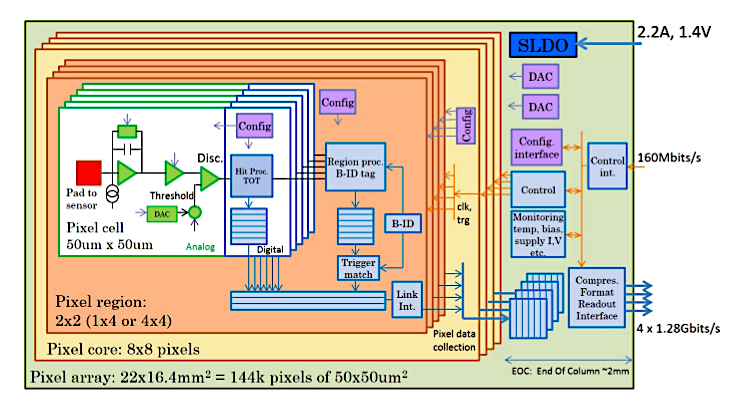
\includegraphics[scale=0.4]{Immagini/ChipBlockDiagram}
\caption{Architettura del chip con bassi livelli di rumore analogico con un sistema di digitalizzazione del ToT a 4 bit. Nello schema sono riportate anche l'interfaccia di controllo, posta nella zona di EOC (End Of Column), l'interfaccia di lettura e il sistema di alimentazione che sfrutta un regolatore di tensione con shunt (Shunt-LDO).}
\label{ChipBlockDiagram}
\end{figure}

La parte cruciale nel sistema di lettura per il tracciatore interno è la progettazione di un chip di lettura dei pixel resistente alle radiazioni. Il diagramma a blocchi del chip è mostrato in figura \ref{ChipBlockDiagram}. 
La carica raccolta su ogni pixel è amplificata, formata e digitalizzata con una risoluzione di 4 bit a 40 MHz, sfruttando l'informazione di ToT (Time Over Threshold)\footnote{Il metodo di ToT consiste nel misurare il tempo durante il quale l'impulso analogico è sopra una certa soglia.}, che viene poi digitalizzata e utilizzata come misura di carica raccolta. 
I segnali vengono memorizzati durante i 12.5 $\mu$s di latenza del trigger\footnote{Si fa riferimento a latenze che si avranno con il trigger di fase II.} e memorizzati localmente in vettori all'interno della regione di pixel (che potrà essere 2 $\times$ 2 o 4 $\times$ 4). 
I dati riguardanti eventi con trigger sono raccolti da questa memoria e dopo un appropriato processo di compressione dati, svolto all'interno del chip, questi sono inviati all'esterno del chip tramite E-links (Electrical links) ad una velocità di 1.28 Gb/s. 
Sempre all'interno del rivelatore sono presenti i moduli di conversione, basati su chip LpGBT, che riversano i dati provenienti da un massimo di 7  E-links in una fibra ottica da 10 Gb/s per il trasporto verso il sistema di acquisizione dati (DAQ), all'esterno del rivelatore. 
I comandi, i dati di configurazione, i segnali di trigger e il clock sono spediti a 2.5 Gb/s verso i moduli di conversione per poi essere convertiti e inviati ai moduli tramite E-links a 160 Mb/s. 
Gli impulsi di calibrazione sono disponibili per tutti i pixel, grazie ad un esteso sistema a doppio impulso che può iniettare due differenti segnali di calibrazione con tempi e livelli programmabili. 
Inoltre è presente la possibilità di monitorare l'attività del chip tramite un 
Sono presenti anche sensori per il controllo della temperatura del chip distribuiti in più punti, in particolare sensori di temperatura sono integrati nella parte del chip che si occupa dell'alimentazione. Questo infatti è il punto con la più alta densità di potenza dissipata, che può variare significativamente in funzione delle configurazioni. 
%All power supply voltages (before and
%after the power regulator) and currents can be measured. In addition, a large number of ana-
%logue operation parameters can be monitored: bias currents for analogue front-ends, band gap
%references, calibration pulse voltages, PLL control voltage, etc. Dedicated features to monitor
%radiation degradation at both single transistor level and digital level (ring oscillators) are also
%included.
Un rapido elenco delle caratteristiche del chip di lettura sono riportate in tabella:

\[
\begin{array}{ll}

\toprule

\midrule

\mathrm{Technology} & \quad 65 \mathrm{nm \quad CMOS}\\

\mathrm{Chip \quad size} & \quad \mathrm{22 mm \times (16.4 mm + 2 mm)} \\

\mathrm{Pixel \quad size} & \quad \mathrm{50 \times 50 \mu m^2, 25 \times 100 \mu m^2)} \\

\mathrm{Number\quad of\quad pixels} & \quad \mathrm{144320} \\

\mathrm{Hit \quad rate} & \quad \mathrm{< 3 GHz/cm^2} \\

\mathrm{Charge \quad resolution} & \quad \mathrm{24 bit \quad ToT} \\


\bottomrule
\end{array}
\]

%si può allungare la lista

Le richieste tecniche per questo nuovo PROC (Pixel Read Out Chip) hanno portato ad l'utilizzo di moderna tecnologia CMOS a consumi ridotti ed alta densità con alimentazione a bassa tensione, circa 1.2 V. Questo fa si che il chip sia alimentato con correnti significative, circa 2.2 A per chip. 
La prima idea potrebbe essere quella di utilizzare convertitori DC-DC locali, ma questa possibilità è esclusa  a causa dell'ambiente ricco di radiazioni, del poco spazio disponibile e del tentativo di limitare il più possibile la quantità di materiale nel tracciatore. 

\begin{figure}
\centering
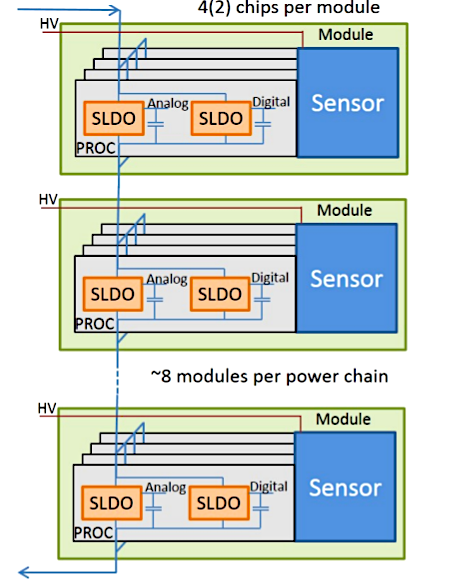
\includegraphics[scale=0.4]{Immagini/serial}
\caption{Sistema di alimentazione seriale dei moduli, ognuno dei quali ha al suo interno 4 o 2 chip in parallelo. Sul chip l'alimentazione è gestita da due SLDO in parallelo, uno per la parte digitale e uno per quella analogica.}
\label{serial}
\end{figure}

La soluzione scelta è dunque quella di utilizzare un sistema di alimentazione seriale, ciò permetto l'utilizzo di un quantitativo minimo di materiale e mantiene a livelli accettabili la perdita di potenza sui cavi. 
La catena è composta da 8-10 moduli ognuno con 2 o 4 chip connessi in parallelo, come si può vedere in figura \ref{serial}. 
All'interno del chip è incluso circuito ottimizzato per l'alimentazione che combina le capacità di uno shunt di corrente e di un regolatore LDO (Low DropOut), chiamato Shunt-LDO (SLDO). 
Come vedremo nel capitolo successivo lo SLDO assicura un consumo di corrente/potenza costante, indipendentemente dal rate di eventi e di trigger. 
Inoltre grazie ad una attenta progettazione è assicurata una suddivisione delle correnti appropriata tra i vari chip posti in parallelo all'interno del modulo. Lo stesso chip al suo interno ha due SLDO in parallelo uno per la parte analogica e uno per quella digitale. 
Questa separazione è resa necessaria per rendere minima l'influenza del rumore della parte digitale su la parte analogica, più sensibile  al rumore.
\chapter{L'alimentazione seriale}
\label{AlimentazioneSeriale}
%L'alimentazione seriale dei moduli è il sistema scelto per l'alimentazione, in grado di rispettare i requisiti per il nuovo tracciatore a pixel di fase due. 
\section{Introduzione}
%Nel capitolo precedente si sono discussi i requisiti richiesti per il tracciatore di fase due: tolleranza agli alti livelli di radiazione, alta risoluzione, riduzione del materiale, etc...
%Per rispettare queste condizioni si è deciso di sviluppare un sistema di alimentazione innovativo e alternativo agli attuali convertitori DC-DC
%\footnote{
%  L'attuale tracciatore utilizza un sistema di alimentazione in parallelo dei moduli, in cui i convertitori DC-DC generano localmente le tensioni necessarie al funzionamento del chip.
%}.
%Questi, infatti, non resisterebbero ai più alti livelli di radiazione della fase ad alta luminosità, nè sarebbero in grado di operare efficacemente in presenza del campo magnetico previsto.
%Il nuovo sistema di alimentazione prevede una distribuzione seriale e sarà gestito, all'interno del chip, da circuiti dedicati prodotti in tecnologia CMOS a 65 nm.

In un sistema di alimentazione seriale il generatore fornisce tensione e corrente ad una catena di carichi, nel nostro caso i moduli, posti in successione. A differenza del sistema di alimentazione parallelo, in cui tutti i moduli si trovano allo stesso potenziale di riferimento e in cui la corrente totale erogata è la somma di quella che scorre nei singoli rami, nel sistema seriale la corrente totale è la stessa per tutti i moduli ed è la tensione di lavoro a cambiare. Dato che i moduli, e quindi i carichi, sono tutti nominalmente uguali, la differenza di potenziale su ciascun elemento della catena è la stessa, ma il riferimento di potenziale cambia localmente.
Inoltre, visto che la corrente viene ``riutilizzata'' in ciascun modulo, il generatore deve fornire correnti minori, rispetto a quelle di un sistema di alimentazione parallelo.
Per questo motivo le dissipazioni nei cavi sono ridotte ed è quindi possibile utilizzare cavi più sottili, riducendo il materiale presente all'interno del tracciatore.
%Questo significa che in ogni elemento scorre la medesima corrente, ma l'intervallo di tensione in cui viene a trovarsi è differente per ciascuno di essi. Fino ad ora il metodo di alimentazione utilizzato era quelo parallelo, tutti i moduli si trovano ad un potenziale comune ma su rami separati, questo implica che nel cavo principale scorre una corrente pari alla somma di quella che passa in tutti i rami e dunque sarà necessario l'utilizzo di un cavo con sezione notevolmente maggiore a quello necessario in una alimentazione seriale.
%Ciò dipende dal fatto che nel caso di alimentazione seriale la corrente sia riutilizzata n-volte riducendo così le perdite di potenza nei cavi, rispetto ad una alimentazione in parallelo, questo consente l'impiego di cavi più sottili riducendo così il materiale all'interno del tracciatore. 
%Inoltre un'alimentazione seriale, rispetto ad una in parallelo, permette di ridurre la potenza dissipata a parità del numero di moduli alimentati.

Infatti è possibile calcolare il rapporto tra la potenza assorbita da n elementi in parallelo e quella di n elementi in serie:
\begin{equation}
\mathrm{W_{parallelo} = n \cdot I \cdot V + (I\cdot n)^2 \cdot R},
\end{equation}
\begin{equation}
\mathrm{W_{serie} = n \cdot I \cdot V + I^2 \cdot R},
\end{equation}
\begin{equation}
\mathrm{\frac{W_{parallelo}}{W_{serie}} = \frac{1+ \dfrac{nRI}{V}}{1+\dfrac{RI}{Vn}}},
\end{equation}
dove R è la resistenza dei cavi, I è la corrente di alimentazione per il singolo elemento e V è la caduta di tensione su ciascun elemento. 

\section{Lo ShuntLDO per l'alimentazione seriale}
\label{sec:SLDOzener}

Nella progettazione del sistema con alimentazione seriale occorre tener conto che il consumo di ciascun ROC, anche se gli elementi della catena sono tutti identici, dipende dallo stato in cui si trova e dalle operazioni che sta eseguendo. 
Il ROC, infatti, è un carico dinamico e l'alimentazione deve essere in grado di erogare abbastanza corrente per far fronte ai picchi di assorbimento dei singoli elementi della catena.
Inoltre, le variazioni dei consumi sono molto veloci e gli alimentatori remoti, detti anche di \textit{back-end}, non sarebbero in grado di compensarle in modo rapido: questi saranno posizionati lontano dall'esperimento e i cavi, lunghi anche fino a $\sim 40-50\m$, introducono un ulteriore carico induttivo non trascurabile.

Per queste ragioni un aspetto chiave dell'implementazione di uno schema di alimentazione seriale \`e che le fluttuazioni del carico, il ROC nel nostro caso, non siano visibili esternamente ma siano gestite localmente facendo s\`i che il carico effettivo visto dalla catena sia costante. Questo pu\`o essere ottenuto implementando, in un appropriato circuito di {\em shunt}, un cammino alternativo per la corrente in quel momento non utilizzata dal ROC, tale che $\mathrm{I}_\mathrm{TOT}\sim\mathrm{I}_\mathrm{ROC}+\mathrm{I}_\mathrm{shunt}\sim\mathrm{cost}$. Inoltre \`e necessario che, in prossimit\`a del ROC, venga effettuata l'opportuna regolazione PoL, che converte l'alimentazione in corrente fornita alla catena, e quindi a ciascuno dei suoi elementi, in una alimentazione in tensione stabile, fruibile dal ROC.
\begin{figure}
\centering
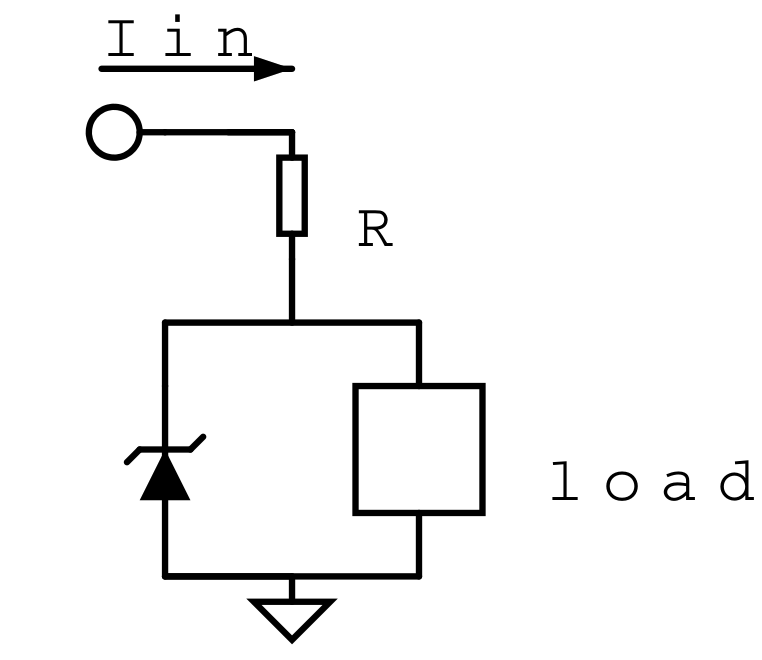
\includegraphics[width=0.5\textwidth]{Immagini/zener2}
\caption{Schema di principio di un circuito regolatore con shunt che utilizza un diodo Zener.}
\label{zener}
\end{figure}
Per flessibilit\`a, versatilit\`a e le motivazioni espresse nella Sezione~\ref{IntroROCIT} \`e auspicabile che questa elettronica addizionale sia integrata nel ROC stesso.

Un possibile schema di principio di tale circuito \`e visibile in~Fig.~\ref{zener} in cui si sfrutta un diodo Zener contropolarizzato per ottenere la stabilizzazione in tensione al carico `load'. Il funzionamento è molto semplice: la corrente in ingresso induce una caduta di tensione sulla resistenza R che, tuttavia, non impedisce di contropolarizzare il diodo Zener oltre la tensione di soglia. A questo punto sarà lo stesso diodo a mantenere la tensione ai capi del carico costante, assorbendo tutta la corrente non necessaria al carico e agendo da shunt. 
Questo schema però presenta problemi operativi nel momento in cui si mettano più regolatori in parallelo, come pu\`o essere necessario fare in applicazioni pratiche, ad esempio, nel caso di un ROC dove servono due tensioni, generalmente diverse, per la parte digitale e la parte analogica, ciascuna fornita da un regolatore diverso, oppure nel caso di un modulo dove pi\`u ROC sono alimentati in parallelo condividendo la stessa corrente in ingresso. Il diodo Zener che, per inevitabili tolleranze di fabbricazione, si trovi all'accensione ad entrare in conduzione prima degli altri assorbir\`a tutta la corrente disponibile con effetti imprevedibili e potenzialmente distruttivi. 

Per ovviare a queste criticità è stato sviluppato un regolatore \textit{Low Drop Out}\footnote{Un regolatore è definito Low Drop Out quando \`e minima la differenza tra la tensione in ingresso e quella in uscita a valle della regolazione; in particolare $\mathrm{V_{dropout}=V_{in}-V_{out}\sim 0.1-0.2 \V}$.} accoppiato ad un circuito di shunt e capace di generare localmente una tensione fissa e di adattarsi dinamicamente all'assorbimento di corrente, denominato {\em ShuntLDO}, con caratteristiche elettriche tali da superare le problematiche a cui si \`e sopra accennato.

Il regolatore ShuntLDO \`e stato inizialmente sviluppato dalla collaborazione Atlas per un suo utilizzo nell'ambito del progetto {\em Insertable B-Layer} (IBL)~\cite{IBL}. Infatti la famiglia di ROC disegnati per IBL, FE-I3~\cite{ROCFEI3} e FE-I4~\cite{ROCFEI4}, implementano entrambi circuiti ShuntLDO dimensionati per correnti totali di $\sim 0.5\A$. Pur tuttavia IBL non implementa uno schema di alimentazione seriale perch\'e ad esso fu preferito uno schema di alimentazione pi\`u tradizionale.

Il disegno dello ShuntLDO \`e stato poi tradotto in tecnologia CMOS a 65~nm dalla collaborazione RD53 per la sfida di HL-LHC: inizialmente in una versione a $\sim 0.5\A$, necessaria per valutare il dispositivo in $65\nm$, per poi arrivare alle attuali versioni dimensionate per correnti massime di $\sim 2\A$.

%Il punto chiave per una alimentazione seriale è che la corrente, che viene fatta scorrere nella catena, sia maggiore o uguale a quella necessaria per alimentare l'elemento con il consumo più alto. 
%Anche nel caso in cui tutti gli elementi della catena siano identici non è vero che avranno pari consumi, gli stessi dipendono dallo stato in cui si trova il chip e le operazioni che esegue. 
%Il chip è dunque un carico dinamico e in qualsiasi momento l'alimentazione deve essere in grado di erogare abbastanza corrente per far fronte ai picchi di assorbimento dei singoli elementi della catena. 
%Dal momento che queste variazioni sono molto veloci l'alimentatore di back-end non può essere in grado di compensarle in modo rapido\footnote{Gli alimentatori sono posizionati lontano dall'esperimentpo e dunque i cavi introducono un ritardo (proporzionale alla lunghezza degli stessi), non è quindi possibile pensare di alimentare la catena in tensione. L'alimentazione dovrà essere in corrente, a livello di chip sarà poi implementato un meccanismo di bilanciamento, che gestisca le variazioni di corrente assorbita.}. Questo è un punto critico che richiede un attento studio. 
%La soluzione al problema consiste nell'implementazione di un regolatore con shunt all'interno del chip, che generi una tensione fissa e si adatti dinamicamente all'assorbimento in corrente. 
%Per quanto detto è necessario che le fluttuazioni di carico date dal chip non siano visibili esternamente, dovranno perciò essere gestite localmente. Il circuito all'interno di ciascun chip incaricato di svolgere questo compito è il regolatore con ShuntLDO.
%\section{Alimentazione seriale con RD53A}
%Partendo dall'idea di utilizzare un'alimentazione seriale, la prima idea che si può avere, è quella di porre singoli elementi in serie, ciascuno dotati di un regolatore, questa configurazione ha però una criticità molto importante: il fallimento di un singolo elemento rende inutilizzabile l'intera catena, inquanto interrompe il flusso di corrente in tutto il ramo. 
%Va perciò implementato un metodo per ovviare a questo problema e anche per mitigare le fluttuazioni di tensione causate dai vari elementi che influiscono significativamente  sulla tensione generata localmente. Il circuito che si occupa di risolvere queste problematiche è un regolatore di tensione ShuntLDO (Shunt Low Drop Out). 
%lo schema consiste in due loop di controllo accoppiati, il primo fa si che il transistor M4 faccia passare tutta la corrente che non è consumata dal carico attivo. Mentre un voltage regulator (A1+M1) assicura che il carico attivo (nel nostro caso RD53A) sia alimentato con una tensione costante, indipendentemente dalla corrente consumata e indipendentemente dalla correte che viene immessa nella catena seriale.
% 
%\section{S$_{unt}$ L$_{ow}$ D$_{rop}$ O$_{ut}$}
%\section{ShuntLDO}


%L'altro punto di interesse nel grafico è quello definito da massima tensione e massima corrente a cui è possibile alimentare il circuito. 
%Una volta sicuri che non sarà mai utilizzata una corrente maggiore del massimo per alimentare il dispositivo, si ha la sicurezza che nemmeno la tensione massima sarà raggiunta.

\subsection{Il principio di funzionamento dello ShuntLDO}

Per descrivere il funzionamento dello ShuntLDO, partiamo da uno schema estremamente semplificato che permetta di comprendere l'idea di fondo, facendo riferimento alla Fig.~\ref{SLDOprova}. 
Come anticipato il circuito di ShuntLDO è alimentato dalla corrente $\mathrm{I_{in}}$, attraverso il nodo $\mathrm{V_{in}}$.  Della corrente in ingresso una frazione $\mathrm{I_\mathrm{ref}}$ scorrerà nel ramo di R3. Questa sarà la corrente di riferimento all'interno dello shunt, vedremo in seguito perché. 
La parte che agisce come regolatore di tensione è il mosfet M1 tramite l'amplificatore A1 che equalizza la tensione sul carico al valore di riferimento $\mathrm{V_{ref}}$ aprendo o chiudendo il gate di M1 e, dunque, facendo scorrere più o meno corrente. 
In assenza della parte di shunt ci sarebbe, quindi, un aumento di $\mathrm{I_{ref}}$ e, conseguentemente, di $\mathrm{V_{in}}$. 
%Per evitare ciò è stato implementato un ramo in parallelo al carico in cui la corrente che scorre è regolata dal mosfet M4 tramite l'amplificatore A3 che, confrontando tramite un opportuno campionamento la corrente nel ramo di M1 e 1000 volte quella nel ramo di R3, ha lo scopo di mantenere la corrente in ingresso a M1 costante. Il complesso costituito da M4 e A3 è la parte attiva dello shunt: A3 fa sì che la corrente nel ramo con M1 sia 1000 volte quella di riferimento che scorre in R3, poiché modifica $\mathrm{I_{shunt}}$ attraverso la variazione della tensione di gate del mosfet M4. 
 Per evitare ciò è implementato il complesso costituito da M4 e A3, cioè la parte attiva dello shunt: A3 fa sì che la corrente nel ramo con M1 sia 1000 volte quella di riferimento, $\mathrm{I_{ref}}$, che scorre in R3, poiché modifica $\mathrm{I_{shunt}}$ attraverso la variazione della tensione di gate del mosfet M4. 
La corrente che scorre in M1 è dunque tenuta costante anche quando si hanno variazioni dinamiche del carico.
\begin{figure}[!htbp]
\centering
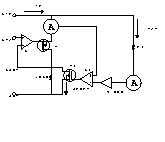
\includegraphics[width=0.75\textwidth]{Immagini/SLDObase}
\caption{Schema di principio dello ShuntLDO.}
\label{SLDOprova}
\end{figure}
 
La Fig.~\ref{SLDOprinciple} mostra graficamente il funzionamento dello ShuntLDO in cui la corrente totale circolante nella catena seriale si divide, in funzione del tempo, in quella indirizzata nello shunt e in quella richiesta dal carico, nelle sue componenti analogica e digitale; \`e esemplificata anche la situazione da evitare, ovvero la richiesta, per tempi prolungati, di una corrente maggiore rispetto a quella disponibile nella catena.
\begin{figure}[!htbp]
\centering
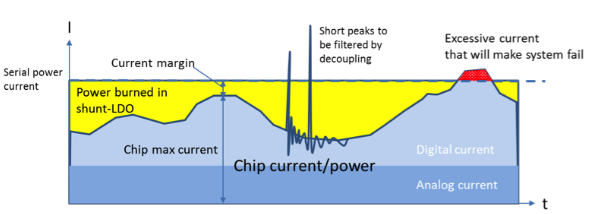
\includegraphics[scale=.5]{Immagini/ShuntRegulatorPrinciple}
\caption{Andamento qualitativo della corrente assorbita da un ROC in funzione del tempo. Mentre la componente analogica \`e sostanzialmente costante, la componente digitale subisce variazioni, anche repentine. Sono da evitare le situazioni in cui il carico richieda, per lunghi periodi di tempo, una corrente in eccesso rispetto a quella circolante nella catena, rappresentata in giallo, mentre picchi veloci possono essere gestiti con opportuno filtraggio.}
\label{SLDOprinciple}
\end{figure}

\subsection{Lo ShuntLDO da $0.5\A$ in 65nm}

 
\begin{figure}[!htbp]
\centering
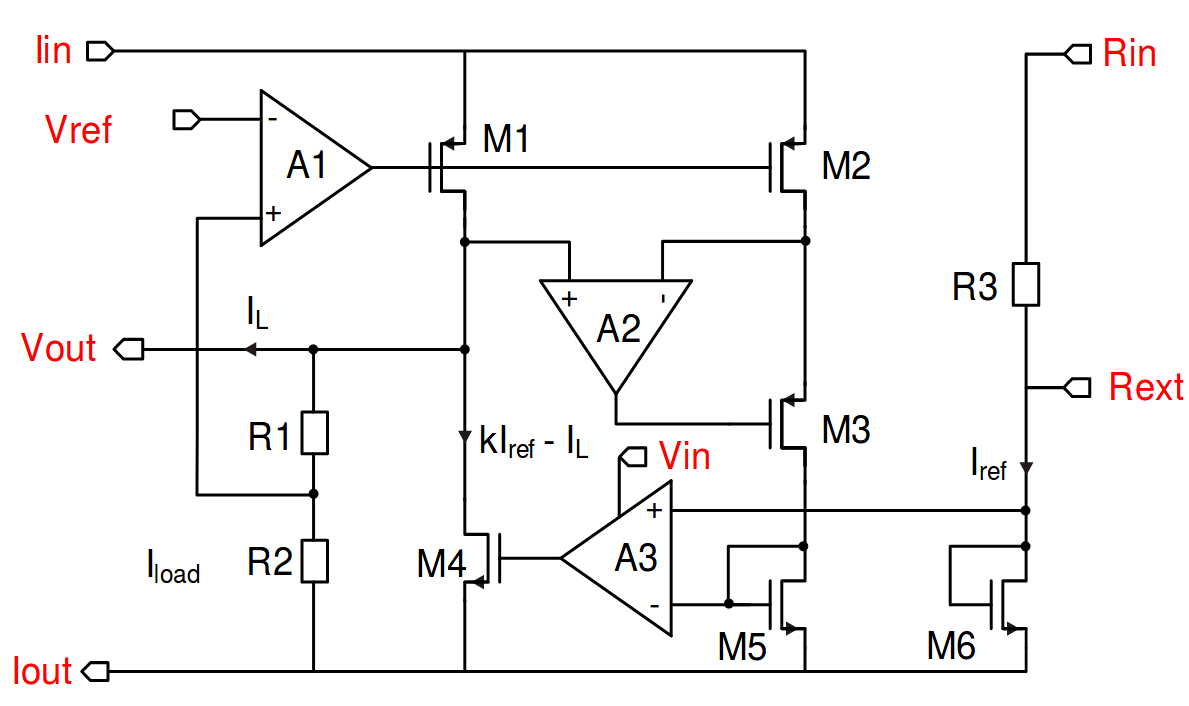
\includegraphics[scale=.3]{Immagini/SLDO5A}
\caption{Circuito semplificato dello ShuntLDO 0.5 A.}
\label{SLDO5A}
\end{figure}

In Fig.~\ref{SLDO5A} \`e mostrato lo schema elettrico del prototipo di ShuntLDO in versione a $65\nm$ dimensionato per $0.5\A$ di corrente massima.
Rispetto a quanto visto in precedenza si hanno alcune differenze, benché l'idea generale di funzionamento rimanga la stessa. 
In questo schema il carico si trova tra i nodi $\mathrm{V_{out}}$ e $\mathrm{I_{out}}$. Grazie al partitore costituito da R1 e R2, con R1=R2, e all'amplificatore A1, $\mathrm{V_{out}}$ risulta essere il doppio della tensione di riferimento $\mathrm{V_{ref}}$.
%\footnote{$\mathrm{V_{ref}}$ non ha niente a che vedere con $\mathrm{I_{ref}}$.}
L'amplificatore A3, invece, confronta la corrente $\mathrm{I_{ref}}$ che scorre nel ramo di R3 (dato che normalmente i nodi $\mathrm{I_{in}}$ e $\mathrm{R_{in}}$ sono connessi) e quella che scorre in M2 e regola il mosfet M4 di conseguenza. 
La coppia di mosfet M1-M2 costituisce un \textit{current-mirror} configurato in modo tale che il rapporto k tra le due correnti sia uguale a 1000 grazie ad una appropriato dimensionamento dei due dispositivi\footnote{
  In un \textit{current-mirror} il rapporto k è uguale a $\dfrac{W_1L_2}{W_2L_1}$ dove $W_1$ e $L_1$ e $W_2$ e $L_2$ sono, rispettivamente, profondità e lunghezza dei due mosfet.
}. 
Grazie al \textit{current-mirror}, quindi, la corrente che scorre in M1 è 1000 volte $\mathrm{I_{ref}}$ e il sistema costituito dall'amplificatore A2 e il mosfet M3 ha lo scopo di migliorare la precisione di questo current mirror.
Questa scelta progettuale definisce il modo in cui lo ShuntLDO è visto esternamente. Infatti la corrente $\mathrm{I_{in}}$ che scorre nello ShuntLDO pu\`o essere espressa come
\begin{equation}
\mathrm{I_{in} \sim k I_{ref} \sim k \frac{V_{in} - V_{thM6}}{R_3}}
\label{eq:IV05amp}
\end{equation}
dove $\mathrm{V_{thM6}}$ \`e la tensione di soglia del mosfet M6. Quindi il generatore connesso al nodo $\mathrm{V_{in}}$ vede un carico resistivo pari a $\frac{R3}{k}$ in serie con una piccola tensione di offset. Il valore di R3 è, quindi, un importante parametro, la cui scelta determina la tensione nel punto di lavoro per una data corrente e, pi\`u in generale, la pendenza di $\mathrm{V_{in}}$ in funzione di $\mathrm{I_{in}}$ nella zona di regolazione, come visibile in Fig.~\ref{fig:IVSLDO} che mostra il caratteristico grafico corrente-tensione dello ShuntLDO e che approfondiremo in seguito.
Il valore di R3 \`e configurabile tramite il terminale indicato con $\mathrm{R_{ext}}$ dove è possibile collegare una resistenza esterna per alterare il valore del resistore integrato nello ShuntLDO.
\begin{figure}[!htbp]
\centering
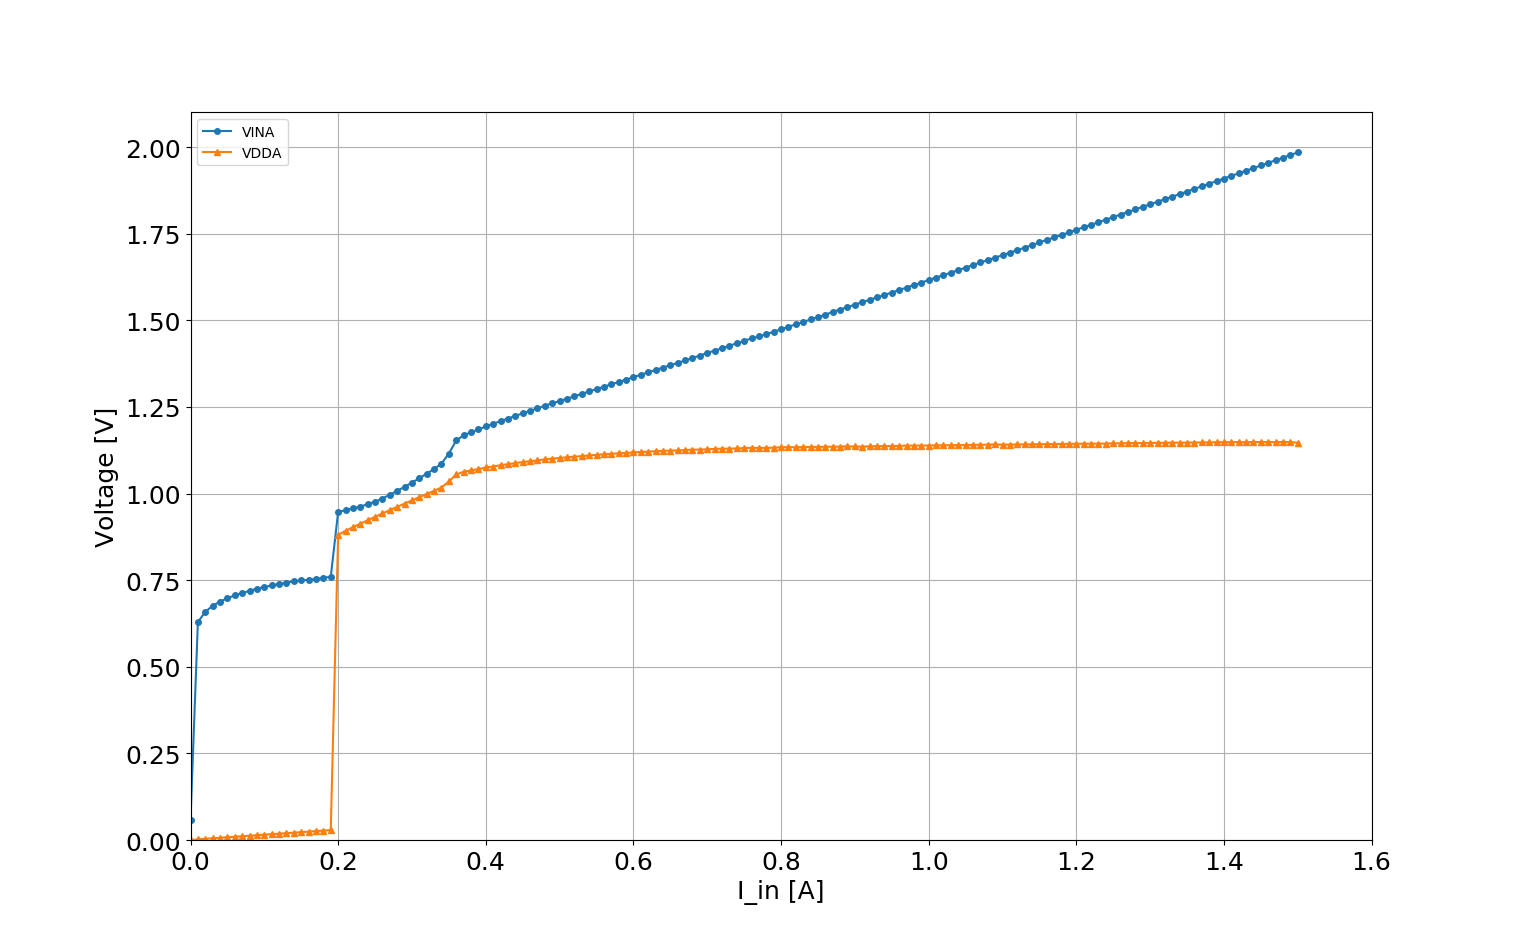
\includegraphics[width=0.99\textwidth]{Immagini/CaratteristicaSLDO.png}
\caption{Caratteristica corrente-tensione per uno ShuntLDO che mostra $\mathrm{V_{in}}$ (curva blu) e $\mathrm{V_{out}}$ (curva rossa) in funzione di $\mathrm{I_{in}}$; la regolazione di  $\mathrm{V_{out}}$ al valore di $\sim 1.15\V$ inizia per $\mathrm{I_{in}}\sim0.4\A$. Al di sopra di questo valore $\mathrm{V_{in}}$ ha una pendenza pari a $\sim\frac{R3}{k}$.}
\label{fig:IVSLDO}
\end{figure}

Per una corretta funzione di regolazione, lo ShuntLDO da $0.5\A$ necessita di una tensione in ingresso minima di circa $1.4-1.5\V$, a fronte di un $\mathrm{V_{out}}$ nominale pari a $\sim 1.2\V$ corrispondente, entro qualche decina di mV, al valore di tensione necessario sia per la componente analogica che per la componente digitale del futuro ROC per l'IT. Il rapporto della differenza tra tensione di ingresso e tensione di regolazione, pari a $\sim 200\mV$, con la tensione in ingresso rappresenta una stima della potenza minima dissipata dallo ShuntLDO pari, quindi, al $\sim 15-20\%$. A parit\`a di $\mathrm{I_{in}}$ e di $\mathrm{V_{out}}$, la scelta della resistenza R3 definisce $\mathrm{V_{in}}$ e, quindi, il punto di lavoro dello ShuntLDO in termini della potenza in eccesso che \`e necessario fornire al regolatore.
\FloatBarrier

% Valori di resistenza maggiori consentiranno, quindi, di operare con correnti minori, con il vantaggio di consumare minor potenza\footnote{
%   La corrente in ingresso è fissata e quella non utilizzata viene dissipata sullo shunt, che diventa conseguentemente molto caldo.
% },
% ma con lo svantaggio di aver minor spazio per le fluttuazioni del carico. 
% Analogamente resistenze minori avranno l'effetto contrario: tensioni minori con correnti maggiori.

\subsection{Lo ShuntLDO da $2\A$ in 65nm}

La successiva versione del prototipo di ShuntLDO a 65nm, progettata per correnti nominali di $2\A$, implementa un ulteriore parametro di configurazione della caratteristica IV per una maggiore flessibilit\`a di utilizzo e configurazione. In particolare \`e stata aggiunta una parte circuitale che permette di calibrare la tensione di offset che definisce la corrente di riferimento nella resistenza R3, pari semplicemente a $\mathrm{V_{thM6}}$, nella versione precedente. Nella Fig.~\ref{SLDO2A}, che mostra lo schema elettrico dello ShuntLDO da $2\A$, \`e visibile il complesso aggiunto per questo scopo costituito dal mosfet M7 controllato dall'amplificatore A4.
\begin{figure}[!htbp]
\centering
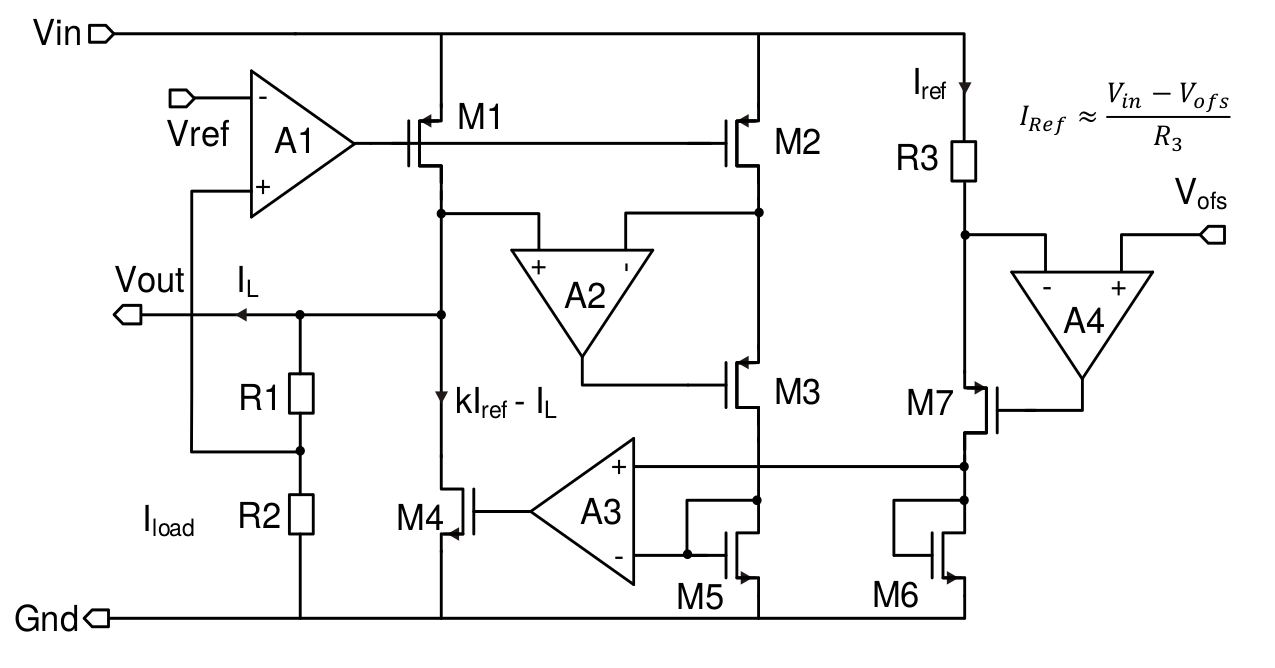
\includegraphics[width=\linewidth]{Immagini/SLDO2A}
\caption{Circuito semplificato dello ShuntLDO 2A.}
\label{SLDO2A}
\end{figure}
%Per quanto visto fin ora non c'è traccia della possibilità di avere un offset.
%In questo tipo di schematico non è prevista la possibilità di avere una $\mathrm{V_{offset}}$.
%Questa caratteristica è stata introdotta nel prototipo a $2A$ riportato in figura \ref{SLDO2A}.
%Facendo riferimento a questa, si può vedere che, rispetto alla versione a $0.5A$, è presente il mosfet M7 sul ramo di R3, il cui gate è controllato da A4.
Grazie alla presenza di questo ulteriore stadio, la corrente di riferimento $\mathrm{I_{ref}}$ diventa, quindi,
\begin{equation}
\mathrm{I_{ref} = \frac{V_{in} - V_{ofs}}{R_3}},
\end{equation}
dove $\mathrm{V_{ofs}}$ \`e la tensione di offset definita tramite l'omonimo terminale, da cui segue una relazione tra $\mathrm{V_{in}}$ e $\mathrm{I_{in}}$ leggermente modificata rispetto alla Eq.~\ref{eq:IV05amp}: 
\begin{equation}
\mathrm{I_{in} \sim k I_{ref} \sim k \frac{V_{in} - V_{ofs}}{R_3}}.
\end{equation}
La tipologia circuitale dello ShuntLDO a $2\A$ \`e, per il resto, invariata rispetto all'omologo a $0.5\A$. La pi\`u ampia tolleranza in corrente \`e ottenuta grazie al dimensionamento dei mosfet M1 e M4 e ad altri dettagli di implementazione del circuito in tecnologia CMOS.

\subsection{Lo ShuntLDO: il circuito equivalente}

Da quanto descritto nelle sezioni precedenti si pu\`o definire regione operativa, o di regolazione dello ShuntLDO, quell'ambito in cui la corrente $\mathrm{I_{in}}$ \`e tale per cui $\mathrm{V_{in}\gtrsim 2\times V_{ref}}+{\cal O}\mathrm{(200\mV)}$, e quindi $\mathrm{V_{out}\sim 2\times V_{ref}}$, e, al contempo, $\mathrm{V_{in}\lesssim V_{in}^{MAX}}$, dove $\mathrm{V_{in}^{MAX}\sim2.0\V}$ è il valore limite per un circuito basato su tecnologia CMOS a $65\nm$. In questa regione il comportamento dello ShuntLDO rispetto ai terminali di ingresso \`e schematizzabile come una resistenza efficace, $\mathrm{R_{eff}}$, definita da $\frac{R3}{k}$, in serie ad un generatore di tensione, $\mathrm{V_{offset}}$. Le variazioni di corrente utilizzata dal reale carico attivo, il ROC nel nostro caso, non sono quindi visibili esternamente al regolatore.
%Un importante caratteristica di questo particolare circuito è che esternamente è visto come una resistenza efficace $\mathrm{R_{eff}}$, in serie ad un offset di tensione $\mathrm{V_{offset}}$, mentre il carico attivo, nel nostro caso il chip RD53A, non è visibile e dunque non lo sono nemmeno le sue le sue variazioni. 
Il comportamento resistivo permette l'utilizzo di più ShuntLDO in parallelo fra di loro, con la corrente che si suddivide in base alla resistenza efficace di ciascuno. La resistenza equivalente risultante \`e quella del parallelo delle resistenze efficaci dei singoli dispositivi superando cos\`i le problematiche descritte nella Sezione~\ref{sec:SLDOzener} che affliggono un tradizionale circuito shunt basato su diodo Zener.

%Inoltre, utilizzando resistenze esterne, è possibile scegliere il valore di $\mathrm{R_{eff}}$ e, conseguentemente, la quantità di corrente che scorre in ciascun elemento posto in %parallelo.

Lo ShuntLDO pu\`o essere implementato direttamente sul ROC stesso e questo ne rappresenta uno degli innegabili vantaggi sia in termini di miniaturizzazione, sia in termini di prossimit\`a al carico reale della regolazione PoL. Come menzionato, gi\`a i ROC per Atlas IBL (FE-I3 e FE-I4) ospitavano due ShuntLDO~\cite{SerialPowering}, uno per la tensione analogica e uno per la tensione digitale. La collaborazione RD53 ha recentemente realizzato il ROC RD53A\cite{RD53A}, il primo prototipo del ROC per HL-LHC, destinato ad essere utilizzato per ampi studi di R\&D. Anche RD53A implementa due ShuntLDO destinati all'alimentazione analogica e all'alimentazione digitale. In condizioni normali questi ShuntLDO lavoreranno in parallelo condividendo la corrente in ingresso. La scelta dei rispettivi valori di $\mathrm{R_{eff}}$ definisce la suddivisione di corrente nei due domini. A differenza dei ROC della passata generazione, in cui il consumo di corrente della parte digitale era marginale rispetto alla parte analogica, in RD53A la componente analogica e quella digitale avranno consumi confrontabili. Per questo motivo i due ShuntLDO sono configurati in modo analogo.

La figura~\ref{VVC} mostra l'andamento della tensione $\mathrm{V_{in}}$ in funzione della corrente totale $\mathrm{I_{in}}$ fornita al ROC assumendo la caratteristica ideale corrente-tensione sopra descritta. Sono, inoltre, evidenziati i valori operativi massimi e la tensione minima di lavoro.
\begin{figure}[!htbp]
\centering
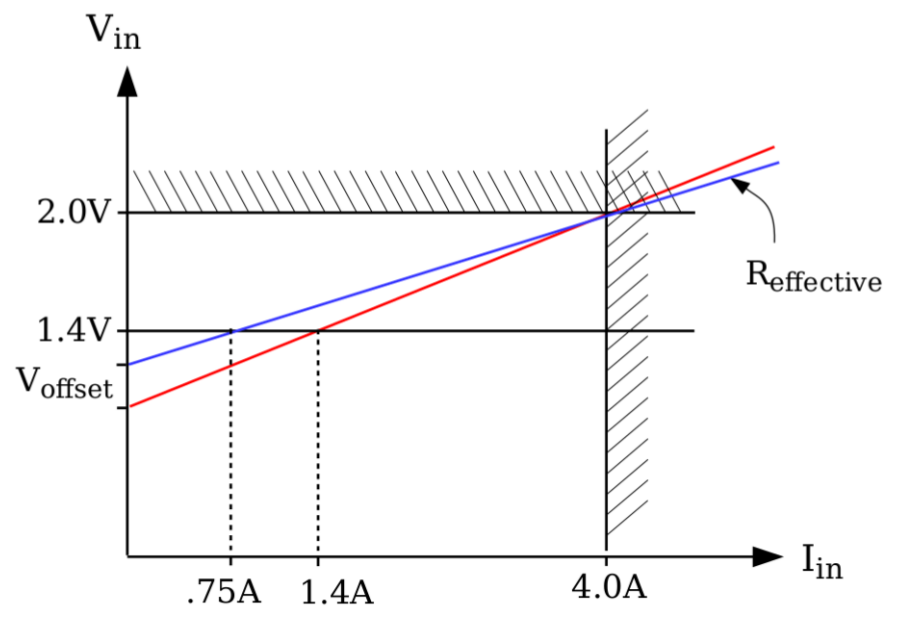
\includegraphics[scale=.3]{Immagini/VoltageVsCurrent}
\caption{Andamento della tensione in funzione della corrente per il ROC. Le zone tratteggiate sono oltre i valori operativi massimi (4.0 A per la corrente e 2.0 V per la tensione), la linea orizzontale a 1.4 V è la tensione minima di lavoro, la pendenza è la resistenza efficace. Combinazioni differenti di resistenza e offset consentono di spostare il punto di lavoro.}
\label{VVC}
\end{figure}
In particolare vengono illustrati i criteri di scelta per i valori di $\mathrm{R_{eff}}$ e $\mathrm{V_{offset}}$: da un lato \`e necessario avere una corrispondenza fra la massima corrente erogabile ($4.0\A$ per il parallelo dato che il singolo ShuntLDO tollera una corrente massima di $\sim2\A$) e la massima tensione ($2.0\V$), dall'altra si dovrà far s\`i che la corrente corrispondente alla tensione minima di lavoro ($1.4\V$) sia sufficiente per il funzionamento del ROC tenendo anche conto di un certo margine necessario per sopperire a eventuali fluttuazioni nei consumi. Nella figura sono visibili due possibili combinazioni $\mathrm{R_{eff}}$ e $\mathrm{V_{offset}}$ rappresentate come due diverse caratteristiche IV.

% Una volta scelti i valori di $\mathrm{R_{eff}}$ e $\mathrm{V_{offset}}$, il consumo in potenza è completamente definito da:
% %La scelta di $\mathrm{R_{eff}}$ e $\mathrm{V_{offset}}$ definisce il consumo in potenza:
% \begin{equation}
% \mathrm{W=I_{in}^2R_{eff}+I_{in}V_{offset}}
% \end{equation}
% %una $R_{eff}$ minore consente di avere minor aumento di potenza all'aumentare della corrente. 
% %e dunque per un corretto funzionamento del chip è possibile utilizzare correnti minori, ovvero lasciando meno margine per le fluttuazioni, proprio perchè con $r_{eff}$ minore le fluttuazioni di corrente
% Accenniamo qui al fatto che la possibilità di modificare $\mathrm{R_{eff}}$ e $\mathrm{V_{offset}}$ permette di progettare diverse configurazioni di consumo in relazione alle necessità.
% Ad esempio si potrebbe avere un \textit{high power mode}, in cui la corrente alla tensione minima di lavoro sia sufficiente a garantire il funzionamento dei chip accesi e funzionanti alle massime prestazioni, come potrebbe essere il caso della linea rossa in figura \ref{VVC}, e un \textit{low power mode} in cui la stessa sia minore poiché non si richiede il funzionamento ``completo'' dei chip, come ad esempio rappresentato dalla linea blu in Figura \ref{VVC}.


% %Con questo tipo di configurazione la corrente erogata dagli alimentatori di back-end deve essere maggiore o uguale a quella necessaria all'elemento con consumo più alto.

% %La posibilità di modificare $\mathrm{R_{eff}}$ e $\mathrm{V_{offset}}$ apre alla possibilità di progettare un modo per avere diverse configurazioni, una di low-power mode e una high power mode. %Al fine di ridurre il consumo di potenza, la resistenza effettiva dello SLDO può avere un offset modificabile. 
% %(Low-power mode configuration, che cosa posso dire...).




\subsection{Schema di catena di alimentazione con ShuntLDO}

\begin{figure}
\centering
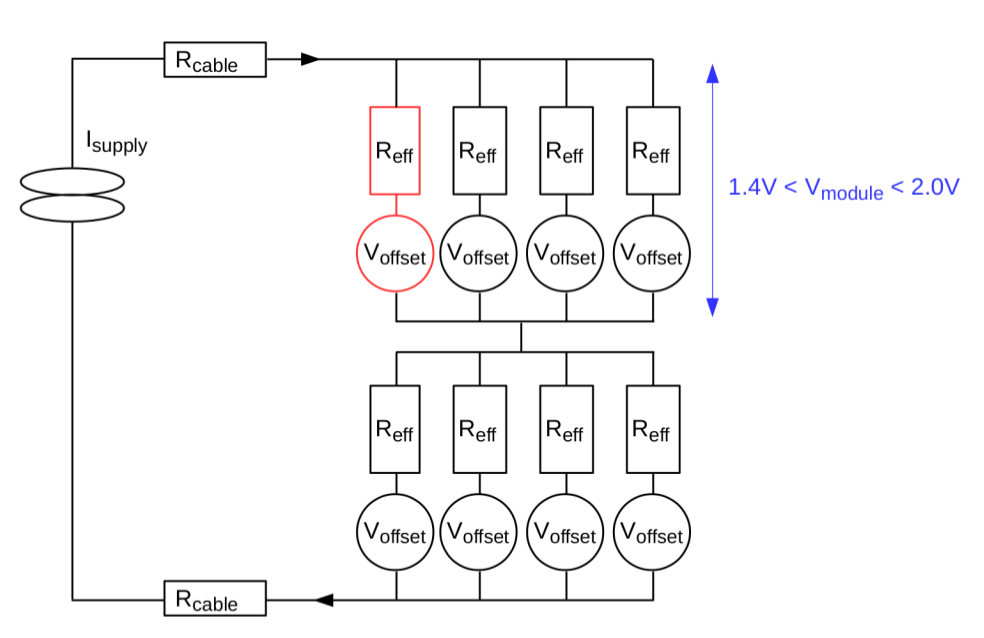
\includegraphics[scale=.3]{Immagini/MultiChipModules}
\caption{Schema di una catena seriale con due moduli da quattro ROC. Il ramo con $\mathrm{R_{eff}}$ e $\mathrm{V_{offset}}$ in colore rosso rappresentano un ROC malfunzionante, non pi\`u attraversato da corrente, come discusso nel testo.}
\label{MCM}
\end{figure}

Il disegno dell'IT prevede moduli 1x2 e 2x2 organizzati in catene di alimentazione seriale composte da 8-12 moduli. I due o quattro ROC di ciascun modulo sono alimentati in parallelo. Lo schema equivalente di due moduli da quattro ROC posti in serie \`e mostrato in Fig.~\ref{MCM} dove $\mathrm{R_{eff}}$ e $\mathrm{V_{offset}}$ rappresentano, a loro volta, il circuito equivalente al parallelo dei due ShuntLDO che sovrintendono, rispettivamente, alla alimentazione analogica e alla alimentazione digitale.

Nella fase progettuale era stata valutata anche la possibilit\`a di implementare l'alimentazione seriale concatenando in serie 8-12 ROC singoli; la catena sarebbe cio\`e costituita da un certo numero di moduli in serie con i ROC di ciascun modulo concatenati in serie anch'essi. Un tale approccio \`e stato scartato perch\'e il sensore si troverebbe ad operare con i pixel polarizzati ad una tensione differente a seconda del ROC a cui sono connessi con effetti che non sono stati valutati a fondo e che, molto probabilmente, richiederebbero uno specifico disegno delle strutture del sensore.

Studiamo adesso l'andamento dei consumi dovuti a più moduli in serie e come cambiano nel caso di un malfunzionamento di uno di questi (per esempio al livello del regolatore) in seguito al quale si azzera la corrente che scorre nel relativo ramo.
%Per meglio comprendere i risvolti dati dall'utilizzo di un'alimentazione seriale con SLDO è interessante fare un esempio dei consumi di questo tipo di alimentazione. 
A titolo di esempio, quindi, prendiamo la situazione in cui si ha una catena seriale costituita da 8 moduli da 4 ROC ciascuno; 
% questo per far si che nel caso un regolatore si guasti , la corrente possa essere assorbita da un altro regolatore all'interno del modulo\footnote{Come già detto i regolatori devono essere in grado d lavorare in parallelo, generare differenti tensioni dalle correnti in ingresso e tenere costante il consumo di corrente tramite lo shunt.}. 
assumiamo che il punto di lavoro scelto corrisponda a $\mathrm{R_{eff}=0.3\Ohm}$ $\mathrm{V_{offset}=0.8}\V$ per il parallelo tra lo ShuntLDO `analogico' e lo ShuntLDO `digitale' dato che la resistenza equivalente di un singolo ShuntLDO \`e tipicamente $0.6\Ohm$.
%Prendiamo come modello la situazione in cui si ha un serie di 8 moduli con 4 chip ciascuno, assumiamo che $\mathrm{V_{offset}=0.8} \V$ e $\mathrm{R_{eff}=0.3}$ $\Omega$ per ciascun chip\footnote{$\mathrm{R_{eff}}$ del singolo SLDO è circa 0.600 $\Omega$, nel chip sono presenti due SLDO in parallelo uno per l'alimentazione della parte digitale ed uno per quella analogica. La $\mathrm{R_{eff}}$ con cui viene visto il chip è dunque la metà, 0.300 $\Omega$.}. 
Con una corrente di lavoro totale richiesta di $\mathrm{I^{ROC}_{in}\sim2.0}\A$ per ROC, equamente divisa tra parte analogica e parte digitale, la corrente totale da fornire all'intero modulo \`e $\mathrm{I_{in}^{modulo}\sim8.0}\A$ corrispondente a $\mathrm{V_{modulo}=1.4} \V$.

Rispetto a questo valore nominale la corrente circolante nella catena deve essere incrementata per avere un opportuno margine di gestione dei picchi di carico da parte del ROC a valle del regolatore. Come si vedr\`a pi\`u avanti, per esempio in Fig.~\ref{LoadTransient}, per avere stabilit\`a della regolazione \`e ragionevole avere un $\sim20-25\%$ di corrente in pi\`u rispetto al valore nominale.
% Per avere un po' di margine incrementiamo la corrente di un 20$\%$, la scelta di dare un margine del 20$\%$, piuttosto che del 40$\%$ è una scelta giustificata qualitativamente dall'ampiezza dei picchi di tensione generati dallo SLDO in concomitanza di un transiente, in figura \ref{LoadTransient} è riportato il valore di picco dell'undershoot/overshoot in funzione del margine di corrente dato su 1 A di alimentazione.
% \begin{figure}
% \centering
% 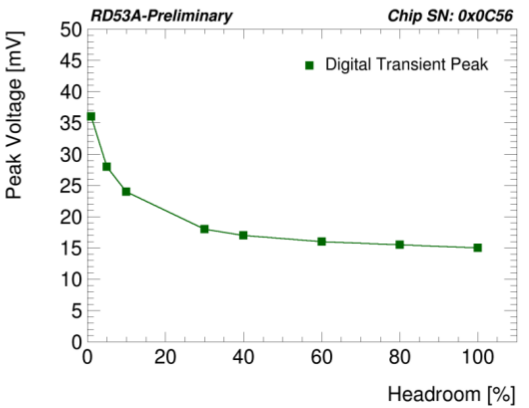
\includegraphics[width=0.75\textwidth]{Immagini/LoadTransientDominik}
% \caption{Il grafico riporta il valore di picco dell'undershoot/overshoot in funzione del margine di corrente dato su 1 A di alimentazione nel caso in cui  i consumi di parte analogica e digitale sono entrambi $\sim$0.5 A, 100$\%$ significa che la corrente fornita al chip è 1 A+1 A.}
% \label{fig:LoadTransient}
% \end{figure}
Conseguentemente $\mathrm{I^{ROC}_{in}=2.4}\A$, $\mathrm{I_{in}^{modulo}=9.6}$ A, $\mathrm{V_{modulo}\sim1.5} \V$ (per un consumo totale di $\sim14.4\W$ per modulo) e, quindi, la caduta di tensione su tutta la catena, formata da 8 moduli, sarà $\sim 12\V$.
%Con una corrente di $\mathrm{I_{in}=2.0}$ A per chip\footnote{Che vale a dire 1 A per ciascuno dei due SLDO presenti nel chip.} ($\mathrm{I=8.0}$ A per modulo) si avrà un $\mathrm{V_{modulo}=1.4} \V$, per avere un po' di margine incrementiamo la corrente di un 20$\%$, la corrente che arriva nei moduli sarà I = 9.6 A. 
%In questa situazione $\mathrm{V_{modulo}=1.52}$ V e dunque la caduta di tensione su tutta la catena formata da 8 moduli sarà pari a $12.16 \V$. Questa non è la caduta di tensione totale, va tenuto conto anche della resistenza dovuta ai cavi, in questo esempio assumiamo valga 2 $\Omega$. 
%Tenendo conto anche della resistenza dovuta ai cavi, che assumiamo valga $2 \Ohm$,
La tensione fornita dal generatore remoto sar\`a $\sim 14-15\V$ perch\`e si dovr\`a tener conto anche della dissipazione sui cavi che si stima compresa tra il $15$ e il $20\%$, comunque ben inferiore ai valori tipici di uno schema di alimentazione parallelo.
%Il generatore sarà infine $\mathrm{V \sim I_{in}^{modulo} \cdot 2 \Ohm +12 \V \sim 31 \V}$.
 
% Dai conti fatti risulta che circa il $60 \%$ della potenza è dissipata sui cavi\footnote{
%  Nonostante il valore elevato in assoluto, bisogna tenere presente che è in realtà un miglioramento rispetto alla situazione attuale, nella quale l'alimentazione è in parallelo.
%}. % sarebbe carino sapere la percentuale di consumo attuale
%La tensione di uscita del generatore è dunque $\mathrm{V=I \cdot 2 \Omega +12.6 \V=31.8 \V}$\footnote{Circa il $60 \%$ della potenza è dissipata sui cavi, questo fatto potrebbe sembrare un pessimo traguardo, in realtà è un miglioramento rispetto alla situazione attuale, nella quale l'alimentazione è in parallelo.}.% sarebbe carino sapere la percentuale di consumo attuale

% Il generatore posto a monte della catena è limitato in corrente e, per fare sì che la potenza erogabile sia maggiore di quella necessaria alla catena, si pone il valore limite della tensione leggermente superiore a quello fin qui calcolato, diciamo ad esempio 34 V.
% %In questo sistema il generatore a monte della catena sarà limitato in corrente, mentre il limite per la tensione sarà posto leggermente maggiore a quello minimo, ad esempio 34 V. 
% %In questo modo la potenza che il generatore può erogare è maggiore di quella necessaria per la catena. 
% La potenza massima che il generatore potrà erogare è, quindi, di $34 \V \cdot 9.6$ A = 326.4 W, per cui, sottraendo la potenza dissipata sui cavi e dividendo per il numero di moduli, si ottiene una potenza per modulo di 17.76 W
% \footnote{
%   Questo a fronte di una potenza assorbita, nelle normali condizioni di lavoro, di
%   \begin{equation*}
%     \mathrm{W_{modulo} = 4 \cdot W_{chip} = I_{modulo} \cdot V_{modulo} = 14.6 W}
%   \end{equation*}
%   per modulo.
% }.
% %Vedremo infatti, come questo sia necessario utile nel caso in cui alcuni chip smettano di funzionare. 
% %La potenza massima erogabile dal generatore sarà $34 \V \cdot 9.6$ $A = 326.4$ W, sottraendo la potenza dissipata sui cavi e dividendo per il numero di moduli si ottiene una potenza per modulo di $17.76$ W. Questo a fronte  di una potenza assorbita, nelle normali condizioni di lavoro, di $\mathrm{W = 4 \cdot W_{chip} = I \cdot V_{modulo} = 14.6}$ W per modulo.

Una accurata valutazione dei malfunzionamenti della catena seriale non \`e ancora stata fatta nell'ambito del progetto IT. Questa infatti non pu\`o prescindere dalla realizzazione di catene prototipali estese, attivit\`a prevista nei prossimi mesi. Ipotizziamo tuttavia che, a seguito di un danneggiamento, gli ShuntLDO di un ROC non siano pi\`u attraversati da corrente come mostrato in Fig.~\ref{MCM} dal ramo con $\mathrm{R_{eff}}$ e $\mathrm{V_{offset}}$ rappresentati in colore rosso.
% Vediamo a questo punto cosa accade nel caso in cui uno dei chip in uno dei moduli sia fuori uso
% \footnote{
%   Dal momento che nel chip ci sono due SLDO, in realtà lo scenario più probabile è che solo uno dei due sia danneggiato.
% },
%Vediamo a questo punto cosa accade nel caso in cui un chip in uno dei moduli sia fuori uso\footnote{Dal momento che nel chip ci sono due SLDO, in realtà lo scenario più probabile è che solo uno dei due sia danneggiato.}.
Ciascuno dei tre ROC dello stesso modulo rimanenti dovrà quindi farsi carico della corrente che non attraversa pi\`u il modulo danneggiato per una corrente totale per ROC pari a $\mathrm{I_{in}^{modulo}/3 \sim 3.2 A}$, valore corrispondente a un terzo di corrente in più rispetto ai $2.4\A$ nominali.
%Dato che l'alimentazione è in corrente, ciascuno dei tre chip rimanenti dovrà assorbire un terzo di corrente in più, dunque la corrente per ciascun chip sarà $\mathrm{I = 9.6A / 3 = 3.2 A}$. 
Di conseguenza cambier\`a anche la caduta di tensione sul modulo in questione che sarà 
\begin{equation*}
  \mathrm{V_{modulo} = 3.2\A \cdot 0.3 \Omega + 0.8\V = 1.8 \V},
\end{equation*}
e la potenza dissipata
\begin{equation*}
  \mathrm{W_{modulo} = 3 \cdot W_{chip} = 3 \cdot I \cdot V_{modulo} = I_{modulo} \cdot V_{modulo} = 16.9W},
\end{equation*}
con un incremento di $\sim2.5\W$ per il singolo modulo, corrispondente a circa il $17\%$. Sul totale della catena, questa maggior richiesta di potenza \`e dell'ordine del \% e quindi marginale. Un ulteriore malfunzionamento porterebbe la caduta di tensione sul modulo a $\mathrm{V_{modulo} = 4.8\A \cdot 0.3 \Omega + 0.8\V = 2.2 \V}$, quindi oltre la soglia di tolleranza in tensione della tecnologia CMOS a $65\nm$ con la conseguenza di avere l'imminente rottura anche degli ulteriori due ROC. La situazione \`e in generale assai pi\`u critica per i moduli 1x2 dato che, in caso di malfunzionamenti, il ROC rimanente si troverebbe a gestire il doppio della corrente nominale.

Si spera per\`o che risulti chiaro da questi esempi che la scelta del punto di lavoro (e quindi di  $\mathrm{R_{eff}}$ e $\mathrm{V_{offset}}$) \`e di importanza fondamentale non solo per le condizioni operative standard, ma anche per la gestione dei malfunzionamenti che spostano localmente il punto di lavoro dei regolatori adiacenti. Non \`e detto per\`o che il meccanismo di rottura pi\`u frequente sia quello in cui il ROC e i suoi regolatori non sono pi\`u attraversati da corrente; \`e ipotizzabile che gli scenari pi\`u frequenti di rottura coinvolgano il solo ROC vero e proprio e che quindi gli ShuntLDO ad esso relativi continuino a funzionare. In questo caso l'inconveniente \`e che tutta la potenza viene dissipata sui mosfet M4 dei regolatori. Per questo motivo nell'implementazione reale dello ShuntLDO sul ROC RD53A e versioni successive, la parte di potenza (essenzialmente il ramo costituito da M1 e M4) \`e ottenuta da un certo numero di repliche connesse in parallelo e distribuite sulla superficie del ROC per evitare un potenziale `hot spot' sia in condizioni standard di funzionamento che in caso di malfunzionamenti.

% Per la catena di 8 moduli l'incremento è, invece, di appena $1.7\%$.
% %Questo porta ad una caduta di tensione sul modulo $\mathrm{V_{modulo} = 3.2 A \cdot 0.3 \Omega + 0.8 V = 1.76 \V}$ e una potenza dissipata $\mathrm{W = 3 \cdot W_{chip} = 3 \cdot I \cdot V_{modulo} = 16.9}$ W, con un incremento di 2 W per il singolo modulo, che corrisponde al $13 \%$. Per la catena di 8 moduli l'incremento, invece, è di appena $1.7\%$. 
% Inoltre ci sarà anche un lieve aumento della tensione erogata dal generatore, $\mathrm{V=I \cdot 2 \Omega +14.08 \V=33.28 \V}$, che è comunque al di sotto dei 34 V
% \footnote{
%   Come visto alla tensione massima di  34 V il generatore riesce a distribuire una potenza di $17.76$ W per ciascun modulo.
% }
% impostati.
%Questo causerà anche un lieve aumento della tensione erogata dal generatore, che però rimarrà al di sotto dei 34 V\footnote{Come visto alla tensione massima di  34 V il generatore riesce a distribuire una potenza di $17.76$ W per ciascun modulo.}.
 %mettere un recap con il senso di questi conti
%Lo studio dell'alimentazione seriale parte dunque dalla caratterizzazione dello SLDO. Componente che sarà poi utilizzato all'interno del chip RD53A per la generazione delle tensioni di alimentazione della parte analogica e digitale. .......continuare discorso....
%Aver chiaro come il chip viene visto esternamente e quali siano i suoi consumi è importante per poter progettare al meglio il sistema di alimentazione seriale.
%capitolo
%\section{Prova}



%At module level, the current to voltage conversion should
%be done using more than one regulator, and by connecting all regulators in parallel. In this
%way, should one regulator fail, the current flow can still be assured by the other regulators on
%module. Although these measures assure a very robust design, extra care has to be taken for
%possible worst case failures, in particular for the case of regulator faults which could cause an
%over-voltage

%\subsection{PCB}
%
%Fino ad ora ci siamo limitati alla descrizione del funzionamento dello SLDO.
%Prima di procedere alla presentazione di misure introduciamo brevemente la (\textit{Printed Circuit Board}) di test, nella cui parte centrale è stato collocato e connesso, con wire-bond, lo ShuntLDO.
%La PCB riportata in figura \ref{PCBTestSLDO} è quella relativa al prototipo di ShuntLDO da 2A.
%La PCB è fornita di tutto ciò che è necessario al funzionamento dello SLDO e all'esecuzione dei test basilari: sono presenti connettori molex per l'alimentazione, jumper di configurazione, pin per misurare varie tensioni, etc....
%\begin{figure}
%\centering
%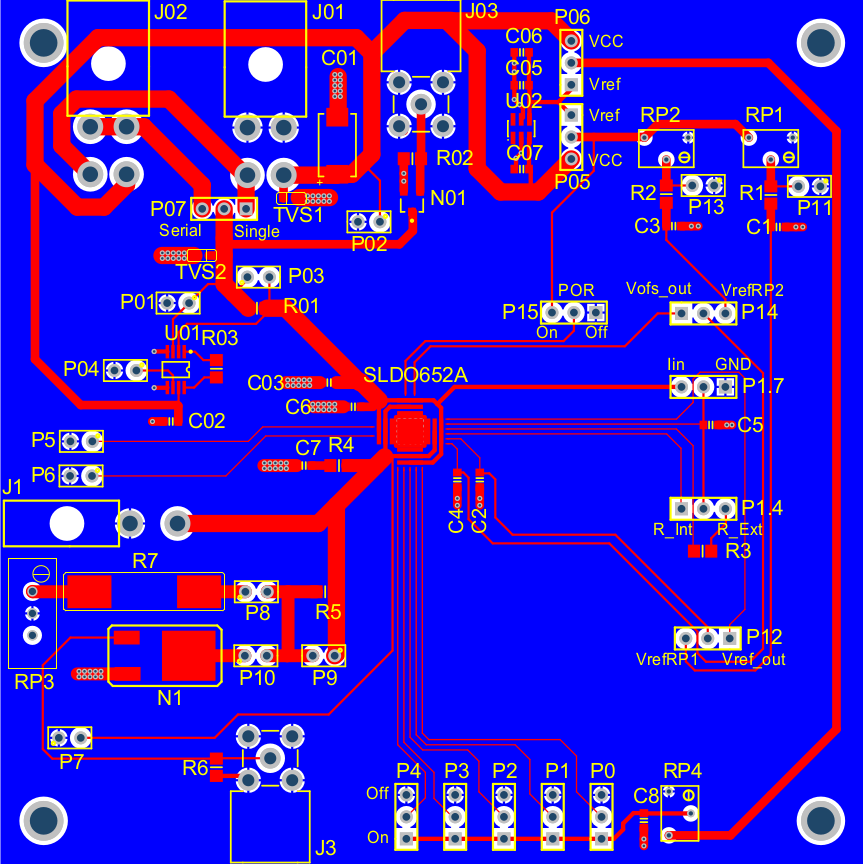
\includegraphics[scale=.3]{Immagini/chipcard}
%\caption{PCB di Test per lo SLDO 2A.}
%\label{PCBTestSLDO}
%\end{figure}


\section{Caratterizzazione dello ShuntLDO da $0.5\A$}

Riportiamo in questo paragrafo alcune misure effettuate sul prototipo di ShuntLDO da $0.5\A$ che hanno permesso di prendere confidenza con i concetti dell'alimentazione seriale e con l'utilizzo dello ShuntLDO.
%A differenza della versione a $2\A$, in questa non è possibile inserire un valore di offset regolabile al $\mathrm{V_{out}}$.

Questo prototipo nasce come un singolo ASIC realizzato per la verifica e la validazione del solo ShuntLDO. Per il test il chip viene montato e microsaldato su una scheda di test progettata appositamente e molto versatile. In Fig.~\ref{PCB05A} sono visibili la struttura e una foto del chip stesso, che contiene tre repliche del circuito ShuntLDO, e il disegno del circuito stampato della scheda di test.
\begin{figure}
\centering
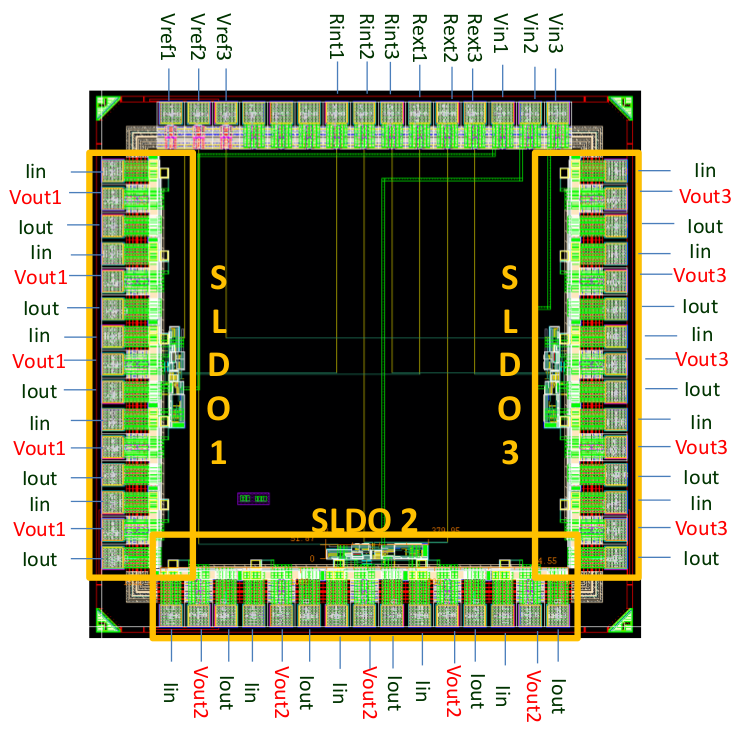
\includegraphics[width=0.32\textwidth]{Immagini/chipSLDO05A.png}
\hfill
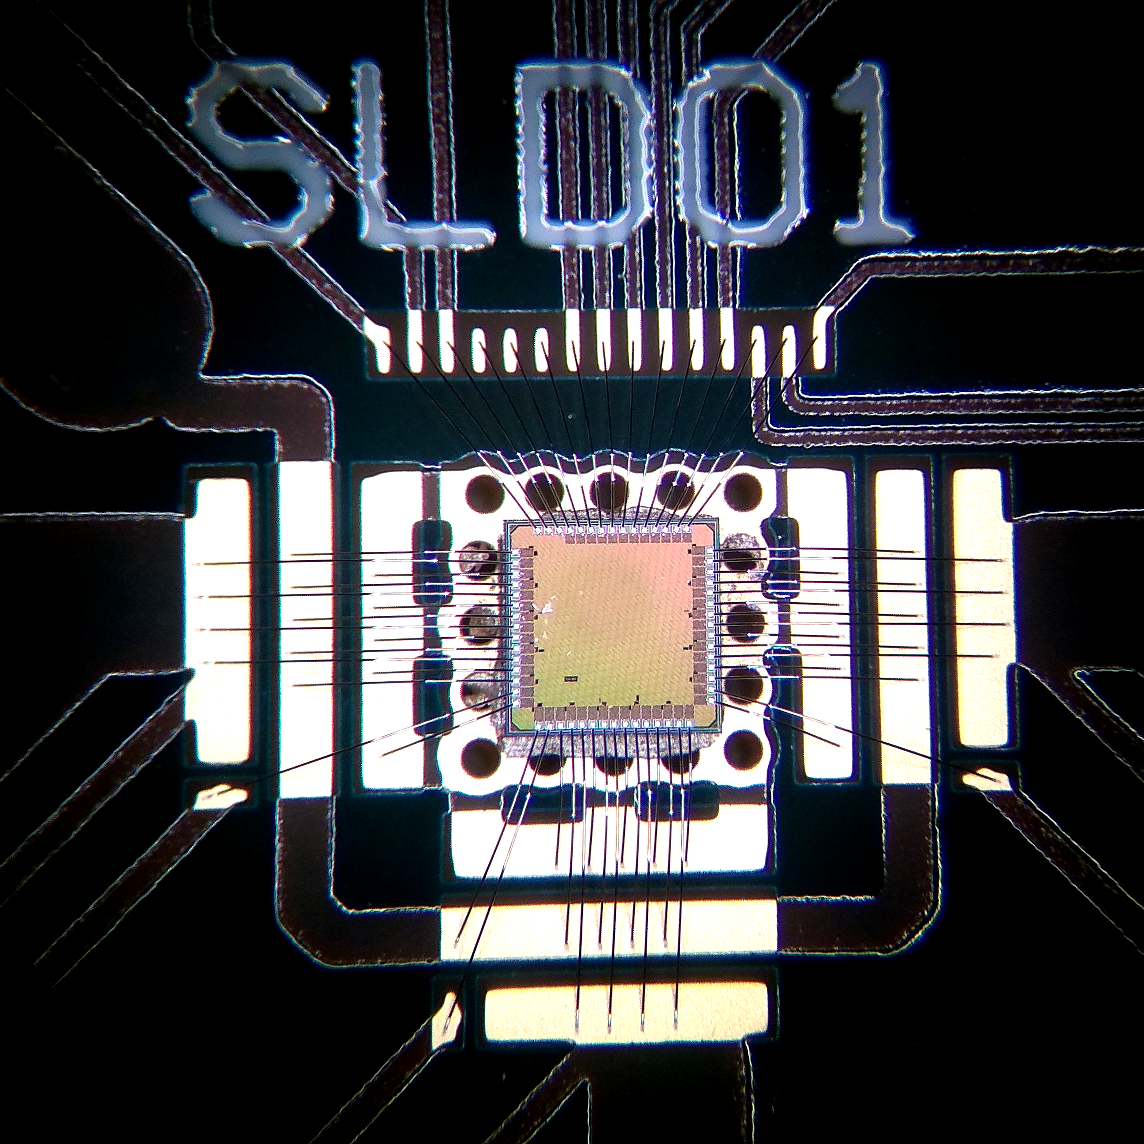
\includegraphics[width=0.32\textwidth]{Immagini/chip05_foto.png}
\hfill
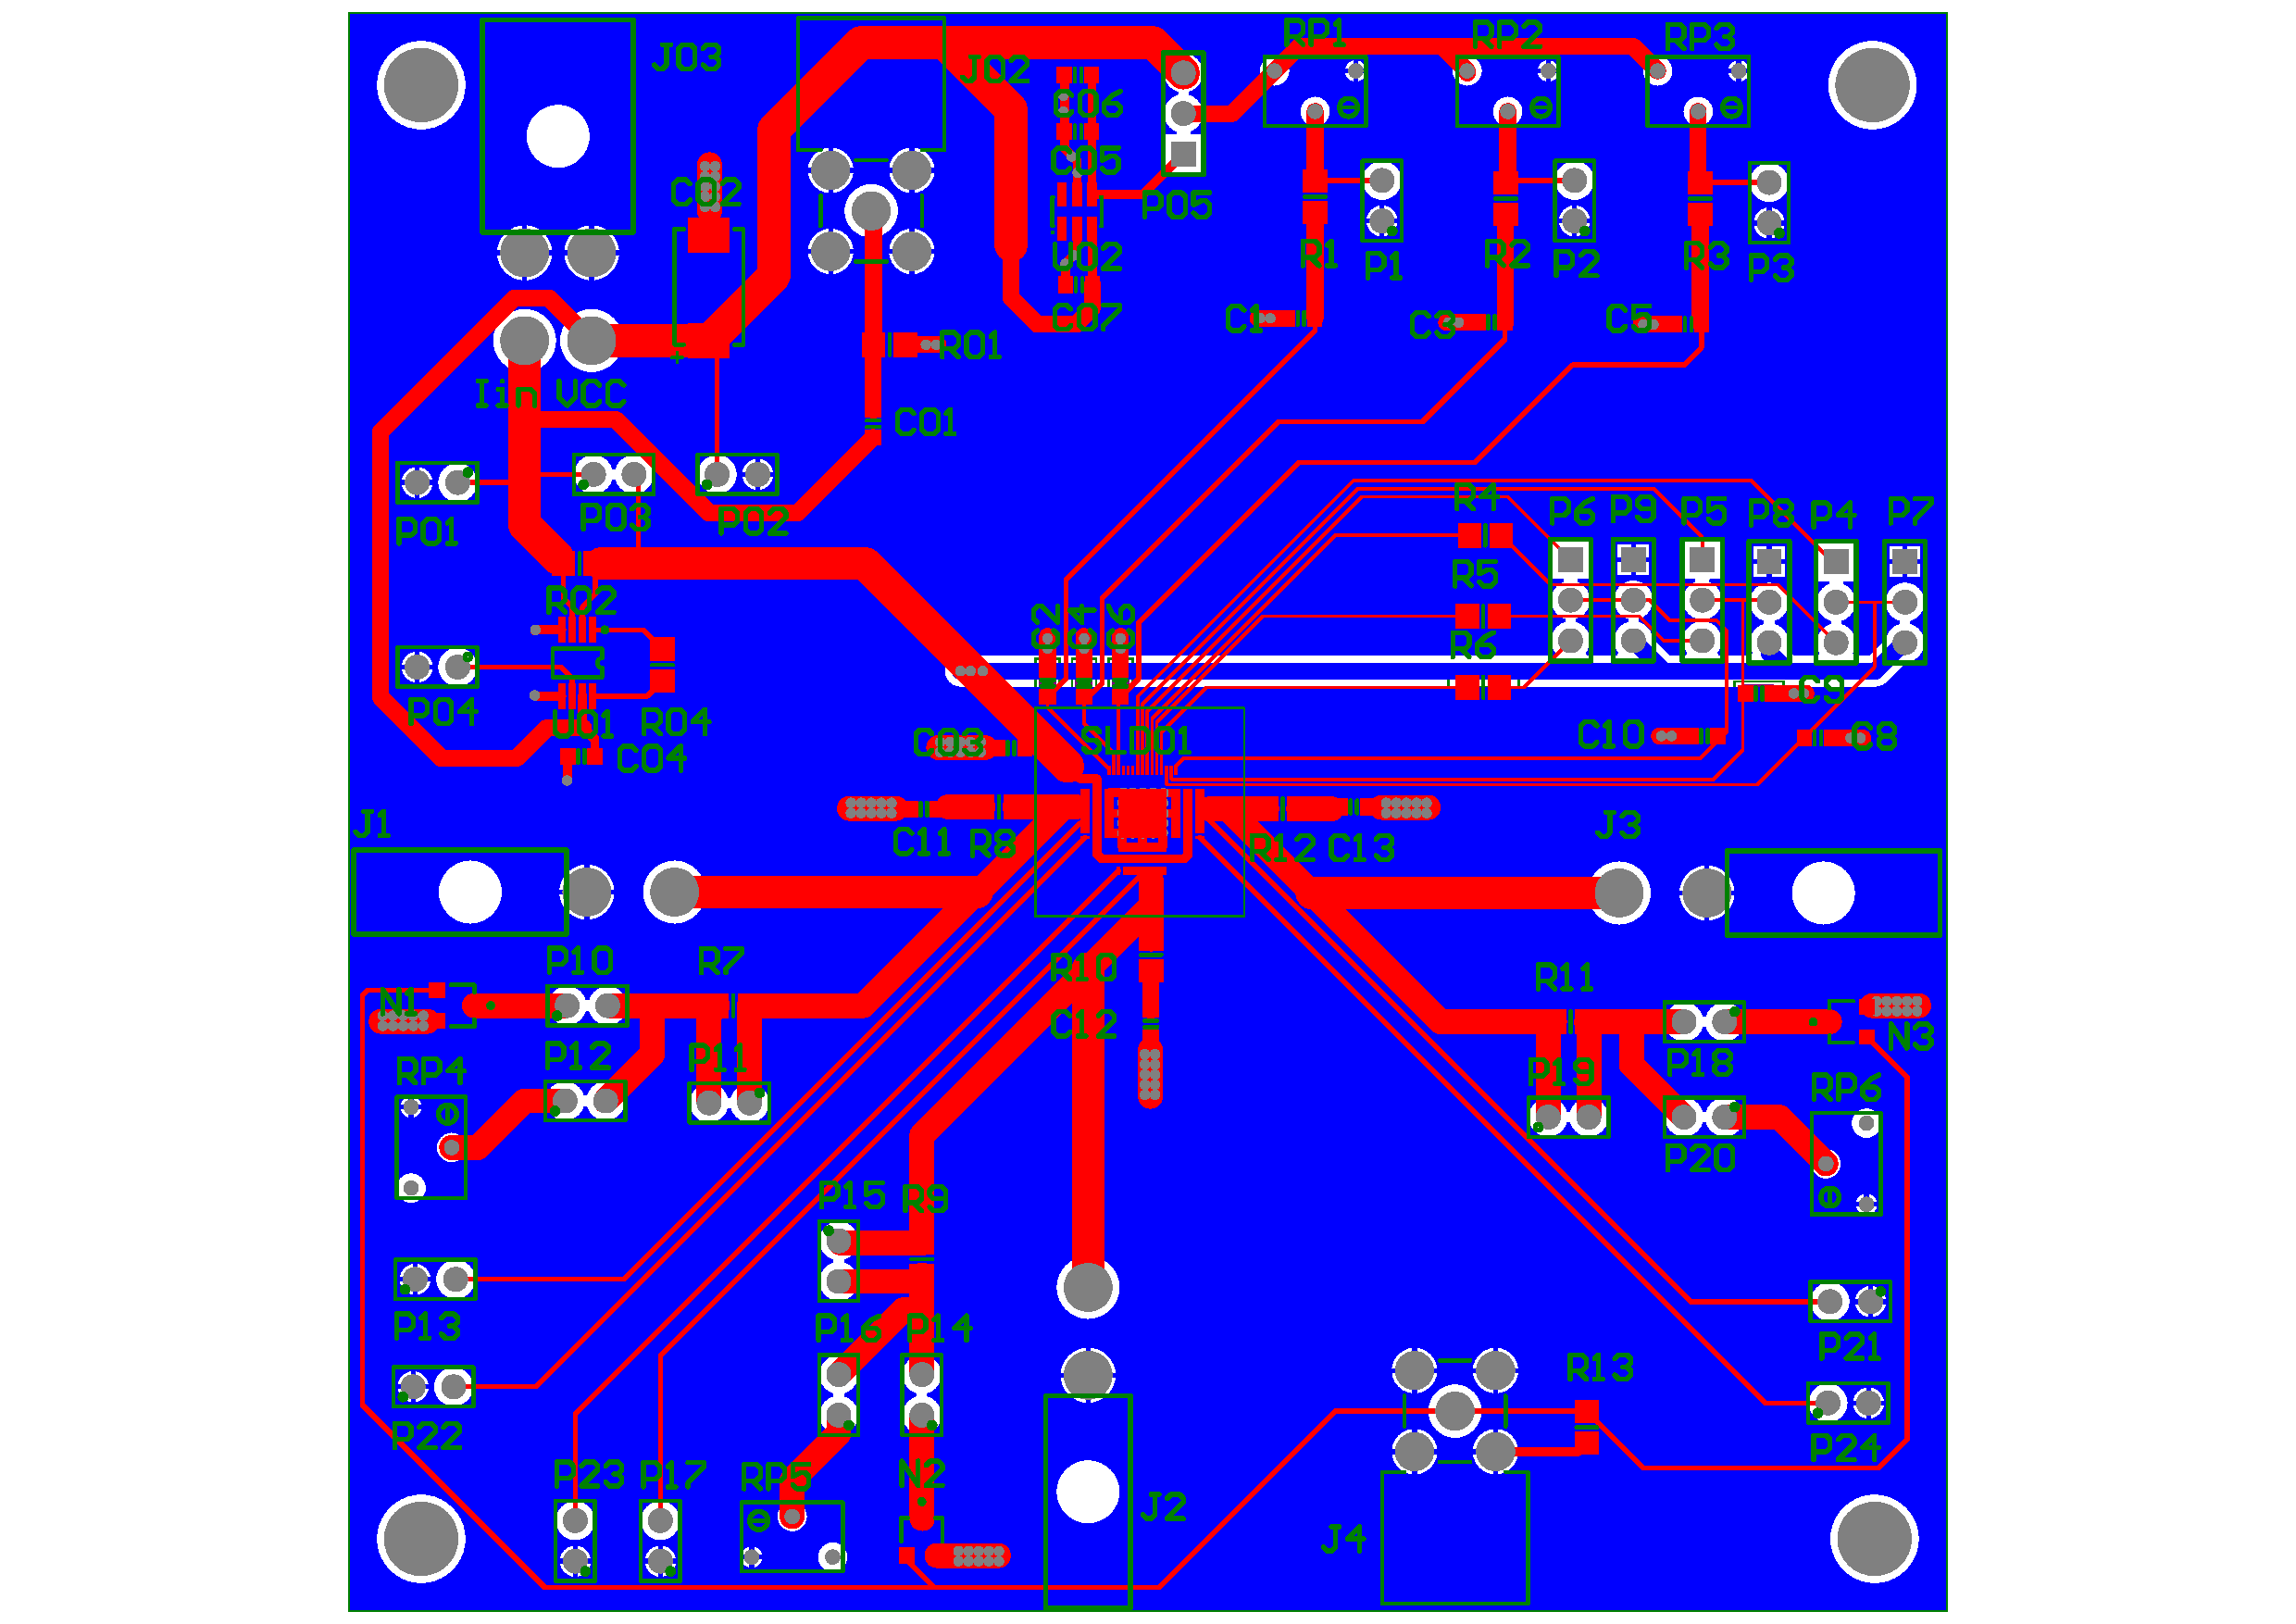
\includegraphics[width=0.32\textwidth]{Immagini/pcb05.pdf}
\caption{La geometria dello ShuntLDO a $0.5\A$ in CMOS a $65\nm$ (sinistra), la foto al microscopio del prototipo montato sulla scheda di test (centro) e il disegno della scheda di test (destra); il chip contiene tre repliche del regolatore e misura circa $2\mm\times 2\mm$ mentre la scheda ha una dimensione di circa $10\cm \times 10\cm$.}
\label{PCB05A}
\end{figure}
Come primo studio abbiamo caratterizzato lo ShuntLDO utilizzando una alimentazione in corrente. Le misure effettuate sono servite ad esaminare l'andamento delle tensioni $\mathrm{V_{in}}$, $\mathrm{V_{out}}$ e $\mathrm{V_{ref}}$ in funzione della corrente in ingresso.

\subsection{Misure in assenza di carico}

\begin{figure}
\centering
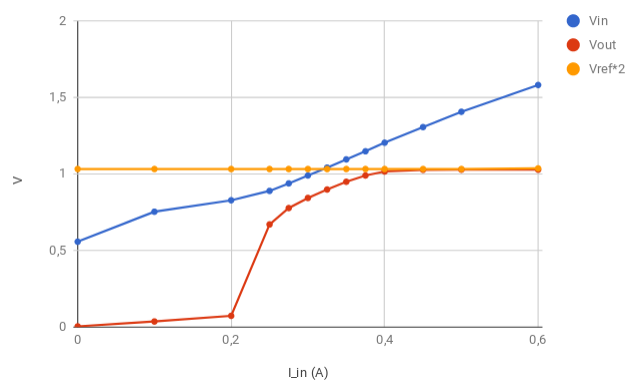
\includegraphics[scale=.5]{Immagini/provaSLDO5}
\caption{$\mathrm{V_{in}}$ (blu), $\mathrm{V_{out}}$ (rosso) e $\mathrm{2\times V_{ref}}$ (giallo) in funzione della corrente di ingresso.}
\label{provaSLDO5}
\end{figure}
In Fig.~\ref{provaSLDO5} è riportato il grafico ottenuto variando la corrente in ingresso, in configurazione senza carico al nodo $\mathrm{V_{out}}$ per cui tutta la corrente fornita dall'alimentazione scorre nello shunt scaldandolo significativamente. Questa misura è di particolare interesse per i confronti con la configurazione in cui è presente un carico, sia esso statico o dinamico.
Dato che la parte a sinistra del grafico corrisponde alla situazione in cui il regolatore non è attivo, consideriamo l'andamento asintotico nella zona di regolazione riportando, in particolare, alcuni valori di interesse:
\[
\begin{array}{cccc}
\toprule
%\mathrm{V_{ref}} & \mathrm{V_{out}} & \mathrm{2 \cdot V_{ref}- V_{out}} & \mathrm{R_{eff}} & \mathrm{V_{offset}} \\
%\midrule
%0.516\V & 1.028\V & 8\mV & 2.0\Ohm & 0.40\V \\
\mathrm{V_{ref}} & \mathrm{V_{out}} & \mathrm{R_{eff}} & \mathrm{V_{offset}} \\
\midrule
0.52\V & 1.03\V & 2.0\Ohm & 0.40\V \\
\bottomrule
\end{array}
\]

\subsection{Misure di due ShuntLDO in serie con carico da 4 $\mathrm{\Omega}$}

%La successiva misura di test che è stata eseguita con questo prototipo di shunt, prima del passaggio alla versione da 2A, è un serie di due SLDO entrambi con un carico resistivo di $\mathrm{4 \Omega}$. In questo caso i due elementi hanno $\mathrm{V_{ref}}$ diversi $\mathrm{V_{ref1}=0.497}$ V e $\mathrm{V_{ref2}=0.553 V}$. 
%Ciò non rappresenta un problema in quanto il comportamento "esterno " non ne è influenzato.
Nella configurazione finale, nel ROC per l'esperimento la tensione $\mathrm{V_{ref}}$ viene generata tramite un regolatore di tensione {\em bandgap}\footnote{Una tensione di riferimento `bandgap' \`e ottenuta tramite una circuiteria che fornisce un voltaggio stabile indipendente dalla temperatura e dalle variazioni della tensione di alimentazione in un ampio margine operativo.} alimentato dalla stessa tensione $\mathrm{V_{in}}$ dello ShuntLDO. 
Per scopi diagnostici, tramite la scheda di test, \`e possibile definire la tensione di riferimento $\mathrm{V_{ref}}$ sia tramite un circuito bandgap integrato sulla scheda che si appoggia a $\mathrm{V_{in}}$, sia in maniera indipendente dalle altre alimentazioni dello ShuntLDO fornendo VCC con una sorgente esterna. 
%Sulla scheda di test è presente un bandgap la cui alimentazione può essere separata da quella dello ShuntLDO. Il compito di questo bandgap è quello di generare la tensione di %riferimento $\mathrm{V_{ref}}$, il cui valore può essere regolato con un potenziometro presente sulla scheda di test.
In figura~\ref{SLDO5Serie} possiamo vedere il confronto fra il diverso comportamento di due ShuntLDO in serie nel caso in cui VCC, la tensione che alimenta il bandgap, sia fornita esternamente e quello in cui VCC sia cortocircuitata con l'ingresso di $\mathrm{I_{in}}$, trovandosi, dunque, a tensione $\mathrm{V_{in}}$.
In questo confronto va tenuto conto che il bandgap presente sulla scheda di test ha un regime di lavoro compreso tra $2\V$ e $18\V$. 
\begin{figure}
\centering
%\subfloat[][Fondo $WW$.]
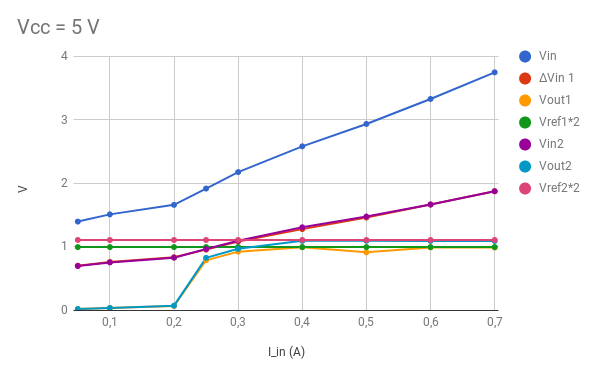
\includegraphics[width=.85\textwidth]{Immagini/SLDO5Serie1}
%\subfloat[][Fondo $WW$.]
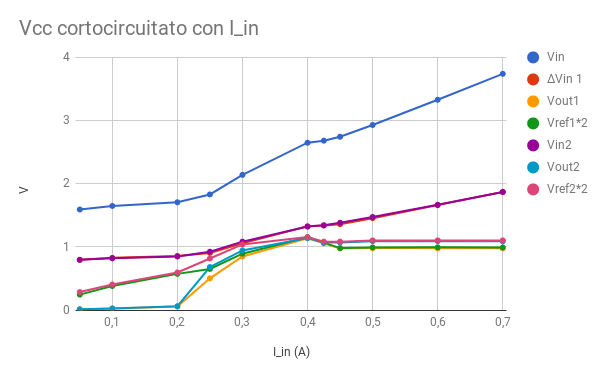
\includegraphics[width=.85\textwidth]{Immagini/SLDO5Serie2}
\caption{Comportamento di due ShuntLDO in serie per due diverse configurazioni di alimentazioni del bandgap integrato sulla scheda che fornisce $\mathrm{V_{ref}}$. In alto i bandgap sono alimentati esternamente, in basso sono alimentati tramite $\mathrm{V_{in}}$.}
\label{SLDO5Serie}
\end{figure}
%Si può notare dai grafici come finto a che la tensione di ingresso non supera circa 1 V il bandgap non riesce a generare il giusto livello di tensione $\mathrm{V_{ref}}$ e ciò ha come conseguenza un $\mathrm{V_{out}}$ non stabile. Si arriva ad una stabilità del $\mathrm{V_{out}}$, solo a tensioni in ingresso più elevate e dunque, con correnti maggiori.
Dai grafici si può notare che, se la tensione di ingresso è inferiore ad $1 \V$, il bandgap non è in grado di generare il giusto livello di tensione $\mathrm{V_{ref}}$, risultando in valori di $\mathrm{V_{out}}$ non stabili. La stabilità di $\mathrm{V_{out}}$ si può ottenere solo con tensioni in ingresso più elevate e, dunque, con correnti maggiori. Questa misura \`e estremamente istruttiva perch\`e illustra l'interazione tra il regolatore e la circuiteria addizionale (in questo caso il bandgap necessario per la tensione di riferimento) nella fase critica dell'accensione. I test di sistema che saranno messi a punto con prototipi pi\`u avanzati dovranno certificare la robustezza dell'approccio utilizzato anche rispetto a queste problematiche.

%magari fare tabellino anche quie
\subsection{Comportamento dinamico}

%\begin{figure}[!hbt]
%\centering
%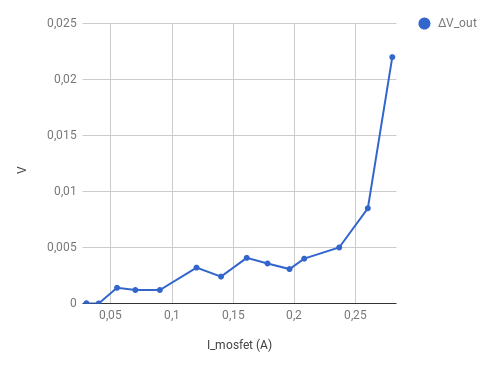
\includegraphics[scale=.5]{Immagini/SLDO5singlepulse}
%\caption{Schema elettrico della circuiteria della scheda di test per lo ShuntLDO a $0.5\A$ dedicata all'emulazione di variazioni rapide del carico grazie ad un mosfet di potenza pilotato da un impulso di gate esterno.}
%\label{SLDO5mosfet}
%\end{figure}
%Prima di passare alla versione da 2A è stata provata una situazione con carico dinamico, per poi riproporla in modo più approfondito ed esaustivo nelle sezioni successive utilizzando però il prototipo da 2A.
Nella scheda di test è presente un mosfet in parallelo all'uscita $\mathrm{V_{out}}$. Il mosfet pu\`o essere pilotato applicando una tensione sul gate. La corrente assorbita dal mosfet si ricava misurando la caduta su una piccola resistenza in serie. Questa circuiteria, il cui schematico \`e visibile in Fig.~\ref{PCB05A}, pu\`o essere utilizzata per emulare variazioni rapide sul carico. 

\begin{figure}[!hbt]
\centering
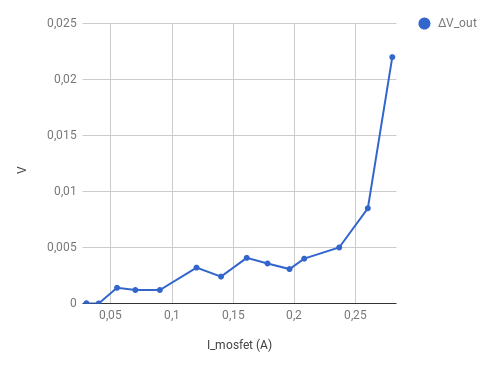
\includegraphics[scale=.5]{Immagini/SLDO5singlepulse}
\caption{Entità degli undershoot in tensione in funzione della corrente assorbita dal mosfet.}
\label{SLDO5singlepulse}
\end{figure}
La prima misura di interesse è la sensibilità di $\mathrm{V_{out}}$ alle variazioni veloci di carico.
In Fig.~\ref{SLDO5singlepulse} è riportato l'andamento dell'entit\`a delle fluttuazioni in basso di $\mathrm{V_{out}}$ ({\em undershoot}) in funzione della corrente assorbita dal mosfet.
Le misure sono state effettuate con una alimentazione in corrente $\mathrm{I_{in} = 0.5 A}$, $\mathrm{V_{ref} \sim 0.5 V}$ e carico resistivo su $\mathrm{V_{out}}$ di $4\Ohm$. 
Conoscere il valore della corrente in ingresso è importante poiché, nel momento in cui il carico dinamico e statico assorbono una corrente maggiore di quella totale in ingresso, il sistema smette di funzionare in maniera corretta.

Gli effetti visibili, nelle situazioni in cui $\mathrm{I_{mosfet} + I_{load} > I_{in}}$ dove $\mathrm{I_{load}}$ è la corrente che scorre nel carico resistivo, non sono direttamente legati alle prestazioni dello ShuntLDO. Al contrario si può vedere dal grafico in Fig.~\ref{SLDO5singlepulse} come gli undershoot siano inferiori a $10\mV$ fintantoché $\mathrm{I_{mosfet}}$ rimane al di sotto di $250\mA$, valore oltre il quale $\mathrm{I_{mosfet} + I_{load} > I_{in}}$. In questo caso $\mathrm{I_{load} = \nicefrac{V_{out}}{R} = 250\mA}$. Queste variazioni di  $\mathrm{V_{out}}$ sono perfettamente compatibili con i requisiti.

%Lo stesso tipo di test può essere eseguito mettendo due ShuntLDO in serie e verificando, al variare del carico di uno, che l'altro elemento della catena seriale ne sia influenzato o %meno.
%ed andando a variare dinamicamente il carico di uno dei due, verificando se esternamente queste variazioni siano visibili, e quindi se influenzino l'altro elemento della catena seriale. 
%Dal momento che l'interesse maggiore è per il prototipo a 2 A questo tipo di misura non è stato riportato nel caso dello SLDO da 0.5A, in quanto lo scopo di questa prima parte è quello di introdurre un certo tipo di approccio e  prendere confidenza con gli argomenti trattati.

\section{Caratterizzazione dello ShuntLDO da $2\A$}
%\begin{figure}
%\centering
%\includegraphics[scale=.3]{Immagini/PCB2A}
%\caption{.}
%\label{PCB2A}
%\end{figure}
%Rispetto a quanto visto in precedenza, nella versione da 2 A è possibile gestire anche l'offset attraverso un potenziometro, che va ad agire sulla tensione in uscita generata dal bangap, la stessa che viene utilizzata anche per generare $\mathrm{V_{ref}}$ regolando un secondo potenziometro. 

Il prototipo ShuntLDO da $2\A$ \`e, analogamente alla versione precedente, un singolo ASIC realizzato a scopo di verifica e validazione che per\`o, a differenza della versione prototipale a $0.5\A$, contiene una sola replica del regolatore. Per questo chip \`e stata messa a punto una scheda di test analoga a quella di cui alla sezione precedente. In Fig.~\ref{PCB2A} sono visibili la struttura e una foto del chip stesso e il disegno del circuito stampato della scheda di test. 
\begin{figure}
\centering
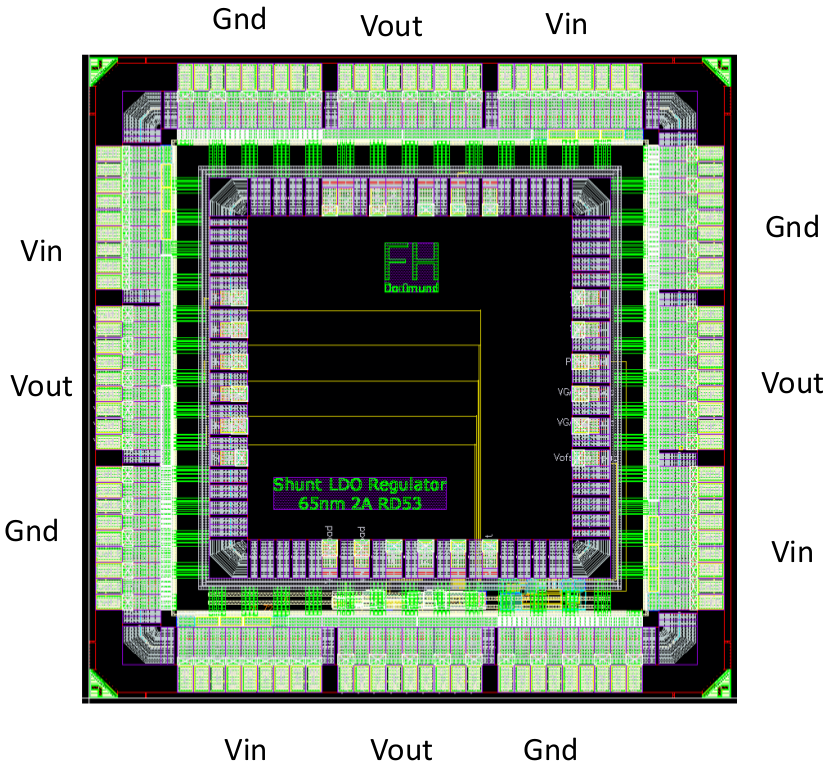
\includegraphics[width=0.32\textwidth]{Immagini/chipSLDO2A.png}
\hfill
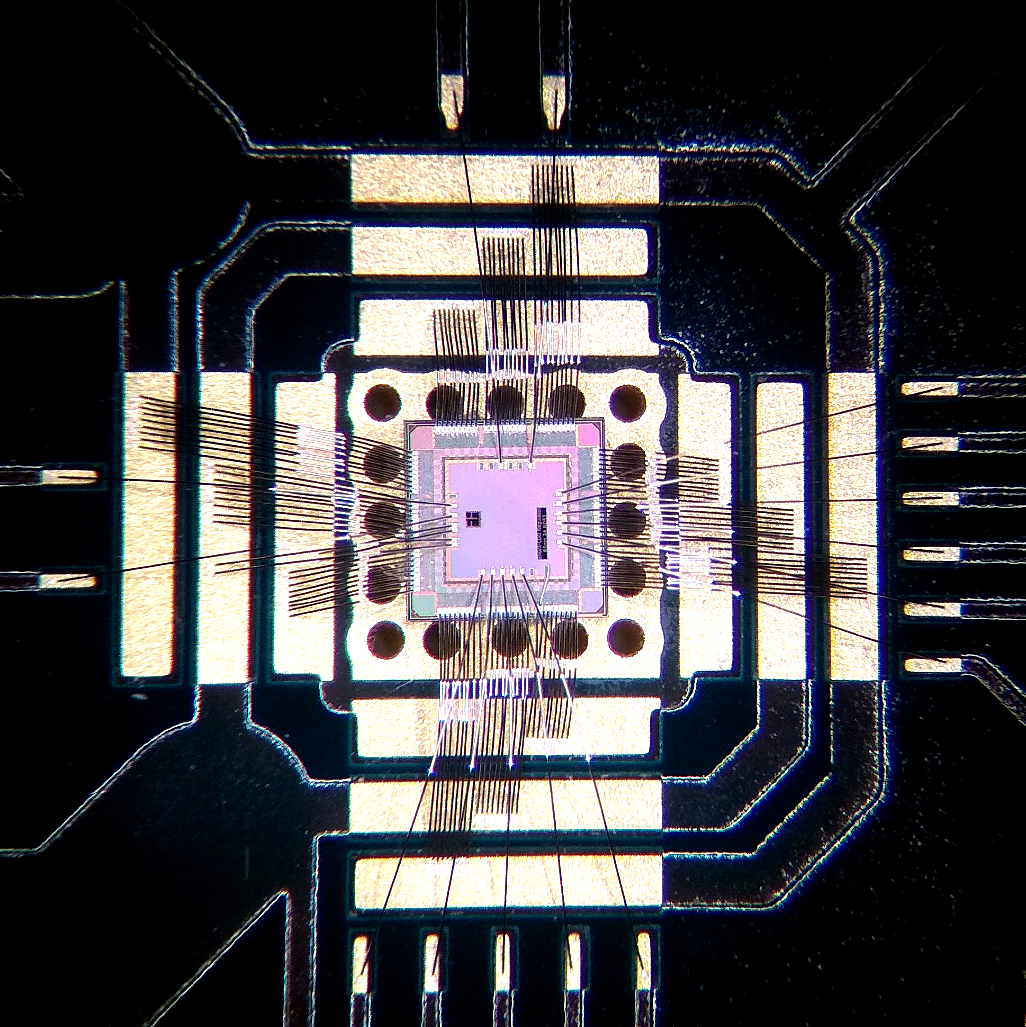
\includegraphics[width=0.32\textwidth]{Immagini/chip2_foto.png}
\hfill
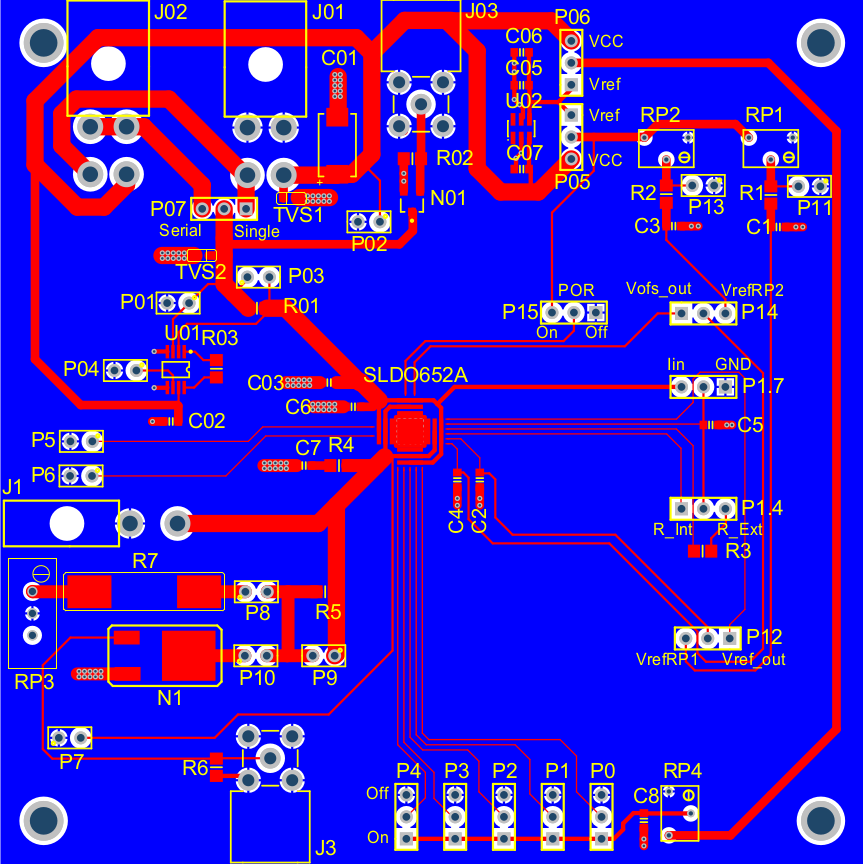
\includegraphics[width=0.32\textwidth]{Immagini/chipcard.png}
\caption{La geometria dello ShuntLDO a $2\A$ in CMOS a $65\nm$ (sinistra), la foto al microscopio del prototipo montato sulla scheda di test (centro) e il disegno della scheda di test (destra); il chip misura $2\mm\times 2\mm$ mentre la scheda ha una dimensione di circa $10\cm \times 10\cm$.}
\label{PCB2A}
\end{figure}
Come abbiamo già detto, un'importante differenza fra la prima versione, con carico massimo da $0.5\A$, e la versione da $2\A$ è la possibilità di modificare $\mathrm{V_{offset}}$ attraverso la scheda di test. $\mathrm{V_{ref}}$ \`e configurabile, tramite bandgap alimentabile anche esternamente, in modo analogo alla scheda di test per il prototipo a $0.5\A$. In questa sezione descriveremo i test effettuati per la caratterizzazione dello ShuntLDO da $2\A$, studiando sia il comportamento con carico statico che dinamico.

\subsection{Comportamento statico}

\par \begin{center} {\huge\bf QUESTO \`E TUTTO DA RIVEDERE } \end{center} \par

La caratterizzazione con carico statico è stata ottenuta usando un carico resistivo da $1\Ohm$ su $\mathrm{V_{out}}$, per avere una corrente sul carico pi\`u elevata, con $\mathrm{V_{ref}} = 0.5 \V$ ottenuto tramite il bandgap alimentato esternamente.
I valori misurati di $\mathrm{V_{out}}$, $\mathrm{V_{ref}}$ e $\mathrm{V_{in}}$ al variare della corrente di alimentazione in ingresso sono mostrati in~Fig.~\ref{SLDO2Astatic}.
%La parte di caratterizzazione statica è di nuovo eseguita andando a variare la corrente di alimentazione in ingresso e al contempo misurando $\mathrm{V_{out}}$, $\mathrm{V_{ref}}$ e $\mathrm{V_{in}}$, figura \ref{SLDO2Astatic}.

\begin{figure}
\centering
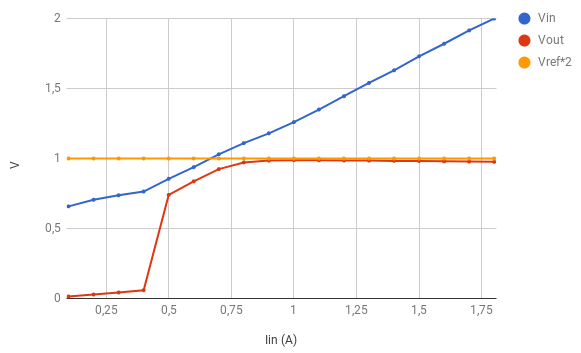
\includegraphics[scale=.5]{Immagini/SLDO2Astaticbis}
\caption{Grafico corrente-tensione che riporta gli andamenti di $\mathrm{V_{in}}$, in blu, $\mathrm{V_{ref}\cdot 2}$, in arancione e $\mathrm{V_{out}}$ in rosso.}
\label{SLDO2Astatic}
\end{figure}

Guardando gli andamenti si può notare come, al momento in cui il circuito si attiva, $\mathrm{V_{out}}$ cerca di raggiungere il valore di $1 \V$ (stabilito attraverso $\mathrm{V_{ref}}$), ma nel far questo è limitato da $\mathrm{V_{in}}$ di cui ne segue l'andamento tra $0.5 \A$ e $0.75 \A$ restando ad una distanza di $\sim 100 \mV$. 
Questo è dovuto alle caratteristiche del regolatore LDO, il quale al massimo può generare tensioni di uscita tali che $\mathrm{V_{dropout}=V_{in}-V_{out}\sim 0.1-0.2 \V}$. 
Considerando gli andamenti asintotici delle tensioni nella zona con $\mathrm{I_{in}}>1\A$ si ottengono i seguenti valori:
%Si può notare che $\mathrm{V_{ref}}$ non è costante nella parte con bassa $\mathrm{I_{in}}$: questo comportamento è dovuto al fatto che, nella fase in cui lo ShuntLDO \`e al di fuori della regione di regolazione, nel ramo di $\mathrm{V_{ref}}$ scorre un po' di corrente che causa una maggiore caduta di tensione del potenziometro e, quindi, una minore tensione all'ingresso di A4 (vd. Fig.~\ref{SLDO2A}).
%Infatti, dato che $\mathrm{V_{ref}}$ si trova all'ingresso del comparatore A1, in una situazione di equilibrio viene confrontata con una tensione molto simile.
%Il comparatore ha una impedenza di ingresso molto grossa e la corrente che scorre in questo sarà, quindi, molto piccola.
%Nella fase di accensione, invece, all'ingresso di A1 si trova una grossa differenza fra + e - e, quindi, una corrente non trascurabile, causa, come visto, della variazione di $\mathrm{V_{ref}}$.

%Questo andamento è stato ottenuto ponendo
%\footnote{Per selezionare il valore voluto è necessario regolare il potenziometro RP1 che si trova in serie al bandgap sulla PBC.} 
%$\mathrm{V_{ref} = 0.5} V$ e applicando un carico resistivo di 1 $\Omega$ a $\mathrm{V_{out}}$. In questa situazione il bandgap è alimentato esternamente con una tensione di 5 V. 
%Come si vede dal grafico \ref{SLDO2Astatic} $\mathrm{V_{ref}}$ non è costante nella parte iniziale, questo può essere dovuto al fatto che nella fase in cui lo shunt LDO non è attivo si ha uno scorrimento di corrente nel ramo di $\mathrm{V_{ref}}$, ciò causa una maggiore caduta di tensione sul potenziometro e quindi una minore tensione all'ingresso di A4. 
%Idealmente, nel ramo di $\mathrm{V_{ref}}$ dovrebbe scorrere una corrente molto piccola in regime di lavoro\footnote{Questo perché nello SLDO il $\mathrm{V_{ref}}$ è in ingresso al comparatore A1 e viene confrontato con una tensione che sarà circa uguale in una situazione di equilibrio. La corrente che scorre tra ingresso + e - sarà piccola, poiché il comparatore in ingresso ha una grossa resistenza.}, mentre al momento dell'accensione, all'ingresso di A1 si ha una notevole differenza tra + e -, e quindi scorrerà una corrente maggiore, questo è causa di una variazione del $\mathrm{V_{ref}}$. Di seguito riportiamo in tabella i valori che si riferiscono al grafico \ref{SLDO2Astatic}: 

\begin{center}
\begin{tabular}{ccccc}
\hline
%$\mathrm{V_{ref}}$ & $\mathrm{V_{out}}$ & $\mathrm{2 \cdot V_{ref}- V_{out}}$ & $\mathrm{R_{eff}}$ & $\mathrm{V_{offset}}$ \\
$\mathrm{V_{ref}}$ & $\mathrm{V_{out}}$ & $\mathrm{R_{eff}}$ & $\mathrm{V_{offset}}$ \\
\hline
%0.500 V & 0.980 V & 20 mV & 0.880 $\Omega$ & 0.40 V\\
0.50 V & 0.98 V & $0.88\Ohm$ & 0.40 V\\
\hline
\end{tabular}
\end{center}
\FloatBarrier
Infine è interessante notare una leggera flessione del $\mathrm{V_{out}}$ all'aumentare  della corrente in ingresso, questo ha stimolato una riflessione su possibili effetti dovuti a differenze di ground tra regolatore e scheda di test.

\subsection{Effetti spuri dell'allestimento di test}
\label{EffettiSpuri}

\begin{figure}[!ht]
\centering
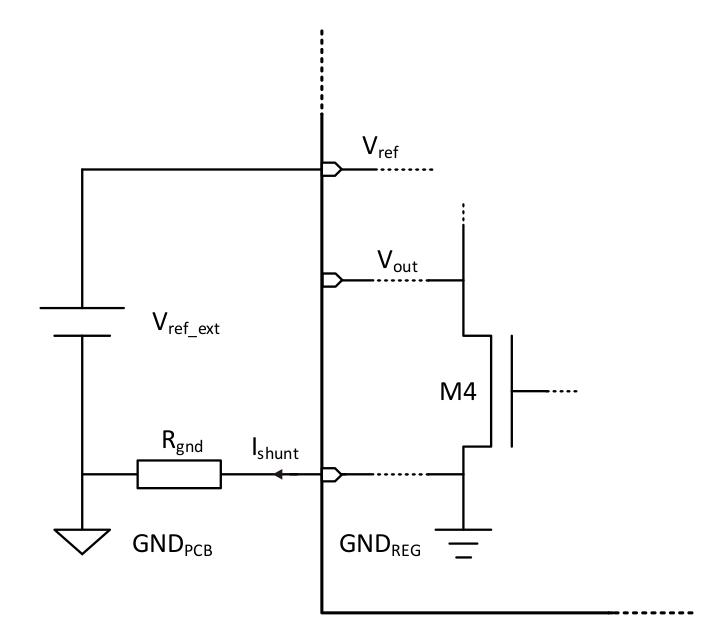
\includegraphics[scale=.3]{Immagini/Ground}
\caption{Porzione dello schema elettrico equivalente del prototipo ShuntLDO e della relativa scheda di test in cui \`e resa esplicita la presenza della resistenza spuria denominata $\mathrm{R_{gnd}}$, associata alle microsaldature, tra $\mathrm{GND_{PCB}}$ e $\mathrm{GND_{REG}}$.}
\label{Ground}
\end{figure}
%Prima di procedere oltre è interessante fare alcune riflessioni.% per porre attenzione su un aspetto che influenza le misure. 
A causa delle maggiori correnti in gioco nel prototipo di ShuntLDO da $2\A$ \`e necessario valutare ed, eventualmente, tenere conto degli effetti dovuti a resistenze spurie presenti nella scheda di test. Per la caratterizzazione del prototipo dello ShuntLDO, infatti, si registrano tensioni misurate su terminali appositamente approntati sulla scheda di test. 
Questi terminali sono connessi a loro volta ai terminali del chip tramite microsaldature che introducono resistenze in serie le quali causano cadute di tensione non necessariamente trascurabili nel caso in cui le microsaldature siano attraversate da correnti elevate. L'entità di queste cadute di tensione dipende dalla resistenza delle microsaldature, dal numero delle stesse\footnote{Le microsaldature si presentano come tante resistenze in parallelo, la resistenza equivalente dipende sia dal valore di resistenza del singolo elemento sia dal numero di elementi in parallelo.} e dalla corrente, e quindi, nel caso di una caratterizzazione con carico statico, si presenta come una differenza di potenziale costante mentre, nel caso di carico dinamico, varia con la corrente. 
Per esempio, come visibile nella Fig.~\ref{PCB2A}, \`e utile introdurre una differenziazione tra il nodo di riferimento locale $\mathrm{GND_{PCB}}$ sulla scheda e il nodo di riferimento locale sul regolatore $\mathrm{GND_{REG}}$. Si pu\`o osservare come la frazione della corrente in ingresso scorre attraverso il transistor di shunt (M4), confluisce nella nodo di riferimento del regolatore $\mathrm{GND_{REG}}$ e da qui attraverso le microsaldature nel nodo di riferimento della scheda di test ($\mathrm{GND_{PCB}}$). 
La resistenza di questa linea, rappresentata in Fig.~\ref{Ground} col resistore $\mathrm{R_{gnd}}$, causa una differenza di potenziale tra $\mathrm{GND_{REG}}$ e $\mathrm{GND_{PCB}}$. Di conseguenza la tensione del nodo di regolazione sul chip $\mathrm{V_{out{\_}REG}}$ sar\`a sempre leggermente inferiore a $\mathrm{2\times V_{ref {\_} PCB}}$, dove $\mathrm{V_{ref {\_} PCB}}$ \`e il valore di riferimento fornito esternamente. In particolare, il valore di tensione $\mathrm{V_{out{\_}REG}}$ prodotto dallo ShuntLDO sarà:
\begin{equation}
  \mathrm{V_{out{\_}REG} = 2 \cdot V_{ref{\_}REG} = 2 \cdot ( V_{ref {\_} PCB} - I_{shunt} \cdot R_{gnd} )}.
\end{equation}
Questo effetto è visibile in~Fig.~\ref{SLDO2Astatic} dove, all'aumentare della corrente $\mathrm{I_{in}}$, si ha una lieve flessione della tensione in uscita $\mathrm{V_{out{\_}PCB}}$ rispetto a $2 \times V_{ref{\_}PCB}$ dovuta al fenomeno sopra descritto salvo effetti all'ordine superiore. Facendo un fit lineare di $\mathrm{V_{out{\_}PCB}}$ nella zona di regolazione si ottiene una pendenza equivalente a una resistenza serie di $0.015\Ohm$ risultante non esclusivamente dalle microsaldature, ma anche al contributo aggiuntivo dovuto alla resistenza delle piste e dei connettori.

%%microsaldature in serie a 1 Ohm trascurabili

%----da qui tagliare?
%Per misure pi\`u accurate la scheda di test prevede anche appositi terminali di monitoraggio $\mathrm{V_{out{\_}Sense}}$ e $\mathrm{I_{out {\_} Sense}}$,
%%indicati sulla scheda di test con P5 e P6, rispettivamente.
%collegati, rispettivamente, a $\mathrm{V_{out{\_}REG}}$ e a $\mathrm{GND_{REG}}$ sul regolatore. Essendo rami in cui non scorre corrente, l'effetto resistivo delle connessioni è eliminato ed è possibile misurare il valore di tensione del GND locale.
%
%\begin{figure}
%\centering
%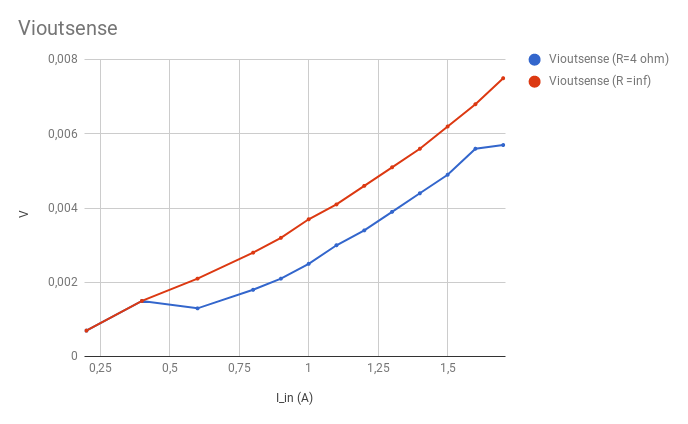
\includegraphics[scale=.4]{Immagini/Viout}
%\caption{Andamento della tensione di $\mathrm{GND_{REG}}$, riferimento locale del chip, rispetto al $\mathrm{GND_{PCB}}$, riferimento locale della  scheda di test, al variare della corrente di alimentazione del circuito per due valori del carico statico connesso a $\mathrm{V_{out{\_}PCB}}$:  $4\Omega$ (curva rossa) e assenza di carico (curva blu). Si precisa che solo per $\mathrm{I_{in}}$ al di sopra di $\sim 750\mA$ il circuito \`e in zona di regolazione.}
%\label{VioutSense}
%\end{figure}
%Si è proceduto quindi a misurare il valore di tensione sul pin $\mathrm{I_{out{\_}Sense}}$ al variare della corrente di alimentazione $\mathrm{I_{in}}$. 
%La misura è stata eseguita per due diversi valori di carico statico connesso al nodo $\mathrm{V_{out{\_}PCB}}$, $4\Omega$ e in assenza di carico, per cui il circuito fra $\mathrm{V_{out{\_}PCB}}$ e $\mathrm{GND_{PCB}}$ è aperto, presentandosi come una resistenza molto grande.
%%$4 \Omega$ e $\infty$, con il valore infinito si intende la configurazione in cui il carico è assente e dunque il circuito tra $\mathrm{V_{out}}$ e GND è aperto, presentandosi di fatto come una resistenza infinita. 
%Gli andamenti di $\mathrm{I_{out {\_} Sense}}$ in funzione di $\mathrm{I_{in}}$ per le due configurazioni sono riportati in Fig.~\ref{VioutSense}.
%La pendenza delle due curve riportate è la stessa, pari a $\sim 4\mOhm$, e ci fornisce un'indicazione del valore resistivo $\mathrm{R_{gnd}}$ delle microsaldature, mentre la separazione tra le due curve risulta alla diversa corrente che lo shunt riversa nel nodo $\mathrm{GND_{REG}}$. Maggiore è la corrente richiesta dal carico, minore è la corrente che attraversa lo shunt e quindi il valore della differenza tra $\mathrm{GND_{REG}}$ e $\mathrm{GND_{PCB}}$.
%La separazione tra le curve, pari a $1\mV$ circa, corrisponde alla caduta di tensione causata dalla diversa corrente che scorre nello shunt nei due casi:
%\begin{equation}
%\mathrm{\Delta V = \Delta I_{shunt} \cdot R_{gnd} = 0.250\A \cdot 4\mOhm = 1\mV}.
%\end{equation}
%All'attento osservatore non sfuggir\`a che le due curve di Fig.~\ref{VioutSense} non sono perfettamente rettilinee. Dato che la misura in oggetto \`e una stima diretta di $\mathrm{I_{shunt}\times R_{gnd}}$ e che l'andamento parabolico \`e presente anche in assenza di carico, situazione in cui $\mathrm{I_{shunt}=I_{in}}$, l'ipotesi \`e che il valore di $\mathrm{R_{gnd}}$ sia indirettamente dipendente da $\mathrm{I_{in}}$ per effetti di temperatura dato che lo ShuntLDO scalda in modo consistente. Queste misure saranno ripetute in condizioni di temperatura controllata per verificare l'ipotesi.
%In figura \ref{VioutSense} è possibile vedere come le due diverse configurazioni di carico influenzino la misura con un offset. 
%Infatti nei due casi la pendenza è la stessa e dà un'indicazione del valore resistivo R dei wire bond, l'offset invece rispecchia il fatto che lo spostamento di tensione è dato dalla corrente che scorre verso il GND del chip, che nel caso in cui il carico richieda più corrente diminuisce.
%Ad esempio ad 1 A con il carico resistivo da 4 $\Omega$, la corrente che effettivamente scorre verso GND nello shunt è 0.75 A (questo nel caso $\mathrm{V_{out} = 1 V}$).

%\par \begin{center} !!! CHE ROBA E'?! CAPTION O ALMENO DESCRIZIONE NEL TESTO !!! \end{center} \par
%
%\begin{center}
%\begin{tabular}{cccc}
%\hline
%$\mathrm{R_{rossa}}$  & $\mathrm{R_{blu}}$ & $\mathrm{Offset_{rosso}}$ & $\mathrm{Offset_{blu}}$\\
%\hline
%4 m$\Omega$ & 4 m$\Omega$ & -1 mV & -2 mV\\
%\hline
%\end{tabular}
%\end{center}

Il valore della resistenza equivalente è molto piccolo e, come detto, dipende in prima approssimazione dal numero di microsaldature.
Fintantoché lo ShuntLDO è utilizzato come circuito a se stante su una scheda di test di test, dato che non ci sono problemi di spazio, è possibile utilizzare un gran numero di connessioni per ridurre al minimo differenze tra $\mathrm{GND_{PCB}}$ e $\mathrm{GND_{REG}}$, in modo da rendere trascurabile il fenomeno. 
Pi\`u in generale, questa istruttiva misura suggerisce che grande cura dovr\`a essere posta nel disegno finale dei moduli dell'IT e in particolare nella ridondanza delle connessioni dal momento che si tratter\`a di dispositivi a corrente relativamente alta in cui gli eventuali effetti spuri vanno attentamente valutati e, se possibile, minimizzati se non completamente eliminati.

\subsection{La regolazione di  $\mathrm{V_{offset}}$}
\label{Voffset}

Torniamo adesso a considerare la possibilità, nella versione da 2 A, di regolare esternamente il $\mathrm{V_{offset}}$. 
Dal momento che $\mathrm{V_{in}}$ dello ShuntLDO deve trovarsi, per funzionare al meglio, $200-300\mV$ al di sopra di $\mathrm{V_{out}=2\times V_{ref}}$, una tensione di offset alta consente di raggiungere la zona di regolazione prima a parit\`a di $\mathrm{I_{in}}$ contenendo cos\`i i consumi totali sempre che la corrente circolante sia sufficiente per le esigenze del carico da alimentare.
Si può verificare questo fenomeno misurando la tensione di uscita del regolatore $\mathrm{V_{out}}$, per diversi valori di $\mathrm{V_{offset}}$, al variare di $\mathrm{I_{in}}$, come mostrato in Fig.~\ref{VoutVsVoffset}.
\begin{figure}
\centering
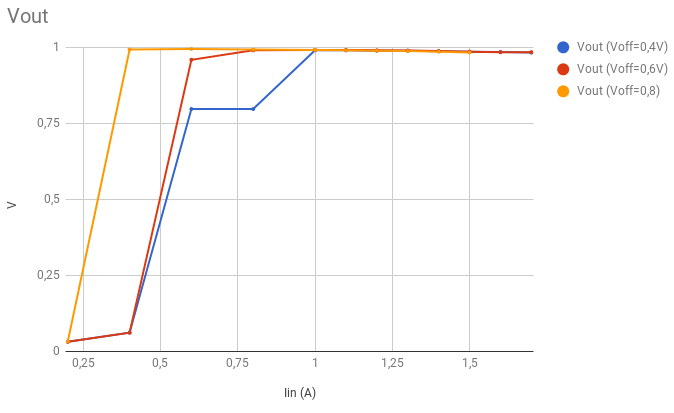
\includegraphics[scale=.4]{Immagini/VoutVsVoffset}
\caption{Andamento di $\mathrm{V_{out}}$ al variare della corrente in ingresso per differenti valori di $\mathrm{V_{offset}}$.}
\label{VoutVsVoffset}
\end{figure}

Dalla misura di $\mathrm{V_{in}}$ al variare della corrente in ingresso mostrata in Fig.~\ref{VinVsVoffset} è possibile ricavare, con un fit lineare nella regione di regolazione del circuito, l'intercetta con l'asse verticale, corrispondente all'offset effettivo dello ShuntLDO. 
\begin{figure}
\centering
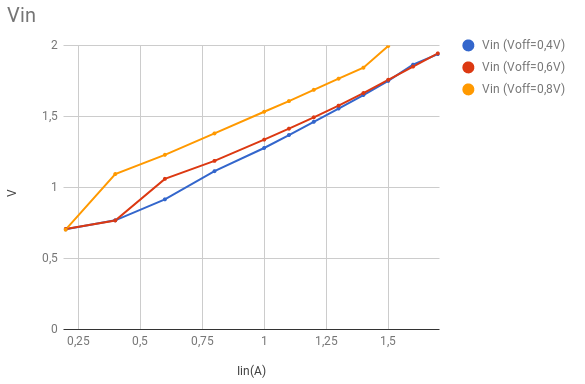
\includegraphics[scale=.4]{Immagini/VinVsVoffset}
\caption{Andamento di $\mathrm{V_{in}}$ al variare della corrente in ingresso per differenti valori di $\mathrm{V_{offset}}$.}
\label{VinVsVoffset}
\end{figure}

%Questi valori sono riportati nella tabella seguente:
I valori ottenuti dal fit delle misure sono:

\begin{center}
\begin{tabular}{rccc}
\hline
Offset nominale & $0.4\V$ & $0.6\V$ & $0.8\V$\\
\hline
Offset effettivo & $0.35\V$ & $0.54\V$ & $0.76\V$\\
\hline
\end{tabular}
\end{center}
%\[
%\begin{array}{ccc}
%
%\toprule
%\mathrm{Offset 0.4 V} & \mathrm{Offset 0.6 V} & \mathrm{Offset 0.8 V} \\
%
%\midrule
%
%0.352 V & 0.539 V & 0.756 V \\
%
%\bottomrule
%\end{array}
%\]

Come si può vedere il valore effettivo è sempre leggermente minore di quello impostato. Questo fenomeno è stato osservato anche nelle misure eseguite sullo ShuntLDO presente all'interno del ROC RD53A e che descriveremo più avanti e non sono ancora chiare le cause. Altra anomalia osservabile nel grafico \`e la differente pendenza delle varie curve che, per\`o, dovrebbe rimanere invariata. I dati mostrano altres\`i una correlazione tra pendenza e offset le cui cause sono anch'esse ignote al momento. %magari mettere referenza a Fig.~\ref{OffsetKaragounis}
\FloatBarrier

%
% -------------------------------------------------------------------------------------------------------
%


\subsection{Comportamento dinamico}

\begin{figure}[!htb]
\centering
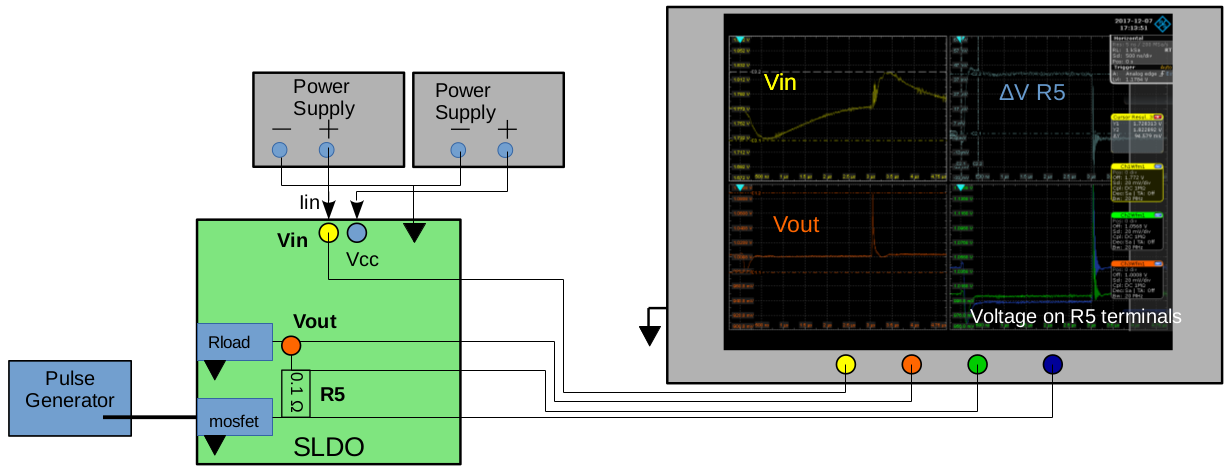
\includegraphics[scale=.3]{Immagini/SetupScheme}
\caption{Schema del setup per lo studio del comportamento dinamico dello ShuntLDO. In grigio sono riportati gli alimentatori e in verde è rappresentata la scheda di test su cui in azzurro sono evidenziati mosfet e carico resistivo, collegato al Gate del mosfet, sulla sinistra, vi è l'impulsatore. Infine, sulla destra è rappresentato l'oscilloscopio attraverso cui sono monitorate le tensioni di ingresso $\mathrm{V_{in}}$, di uscita $\mathrm{V_{out}}$ e quelle ai capi di R5.}
\label{Setupscheme}
\end{figure}

Fino ad ora abbiamo visto la caratterizzazione con carico statico dello ShuntLDO a $2 \A$.
\`E fondamentale studiare il comportamento dello ShuntLDO in risposta ad una variazione dinamica del carico, focalizzando l'attenzione sulla velocità dello shunt nel riequilibrare il consumo in corrente. 
%Oltre alla caratterizzazione statica un punto fondamentale è studiare il comportamento dello ShuntLDO in risposta ad una variazione dinamica del carico, andando a focalizzare l'attenzione sulla velocità dello shunt nel riequilibrare il consumo in corrente. 
La risposta dinamica dipende da molti fattori quali: il punto di lavoro a cui si trova lo ShuntLDO, il tempo in cui avviene la variazione di carico e l'entità di tale variazione. 
Il circuito è alimentato tramite un generatore di corrente a $1.5 \A$ e la tensione di riferimento per $\mathrm{V_{out}}$ è posta pari a $\mathrm{Vref=0.5 \A}$.%, ci aspettiamo una tensione all'uscita di $1 \V$.
Al fine di introdurre un carico dinamico, in parallelo al carico statico, è presente sulla scheda di test un mosfet in serie ad una resistenza, R5, di $0.1 \Omega$.
La corrente assorbita dal mosfet, indicata con $\mathrm{I_{mosfet}}$, può essere calcolata misurando la caduta di tensione su R5 ed è regolabile attraverso la tensione applicata al gate, in questo caso collegato ad un generatore di impulsi esterno.
A seconda dell'ampiezza del segnale inviato al Gate del mosfet si avrà una maggiore o minore corrente che scorre tra Drain e Source. 
Il setup di queste misure è rappresentato schematicamente in Fig.~\ref{Setupscheme}.
%: sulla sinistra in verde, la scheda di test; in grigio sono riportati gli alimentatori; sulla destra l'oscilloscopio con cui sono misurate la tensione in ingresso $\mathrm{V_{in}}$
%\footnote{
%L'alimentazione dello ShuntLDO è comunque in corrente.
%}, rappresentata in giallo, la tensione in uscita $\mathrm{V_{out}}$, in arancione, e le tensioni agli estremi della resistenza R5 in azzurro; infine, sulla sinistra della scheda di test, collegato al gate del mosfet, è presente un generatore di impulsi. 
La durata dell'impulso da mandare al Gate del mosfet è stata scelta tale da mantenere fronte di salita e discesa indipendenti, in modo da osservare separatamente gli effetti dovuti all'uno e all'altro.
%Infatti, in una situazione in cui il carico del regolatore è il chip le variazioni sarebbero di minor durata rispetto alla lunghezza dell'impulso utilizzato in queste misure.
Ad ogni modo lo scopo di queste misure è quello di vedere gli effetti al passaggio da un certo consumo di corrente ad uno maggiore e viceversa ed un impulso di breve durata sovrapporrebbe questi due effetti, non permettendo di valutarli correttamente, in quanto i contributi sono opposti e, su tempi brevi, si cancellerebbero a vicenda.
In queste misure l'attenzione sarà focalizzata su variazioni di $\mathrm{V_{in}}$ e $\mathrm{V_{out}}$ in ampiezza e sul tempo di recupero al variare di $\mathrm{I_{mosfet}}$ per una data $\mathrm{R_{load}}$.

L'introduzione del carico $\mathrm{R_{load}}$ in parallelo alla resistenza connessa a $\mathrm{V_{out}}$ è possibile andando a modificare la configurazione della scheda di test.
Dalle prime misure con l'oscilloscopio è possibile vedere che che l'utilizzo del mosfet come carico dinamico non è esente da fenomeni di alterazione dei segnali, ciò rende difficile una loro corretta interpretazione. 
\begin{figure}
\begin{subfigure}{.5\textwidth}
  \centering
  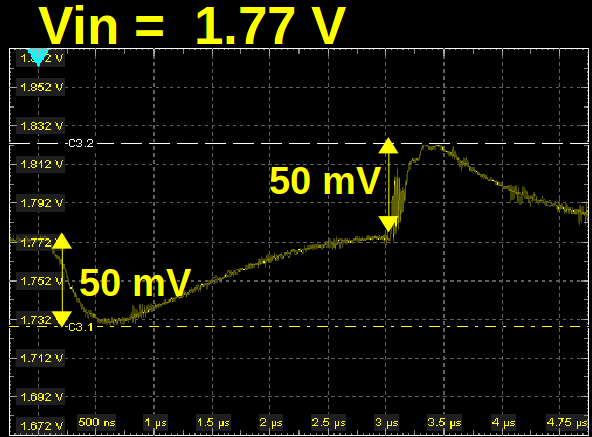
\includegraphics[width=.96\linewidth]{Immagini/zoomTransientTest1}
  \caption{ }
  \label{TransientTest:sfig1}
\end{subfigure}%
\begin{subfigure}{.5\textwidth}
  \centering
  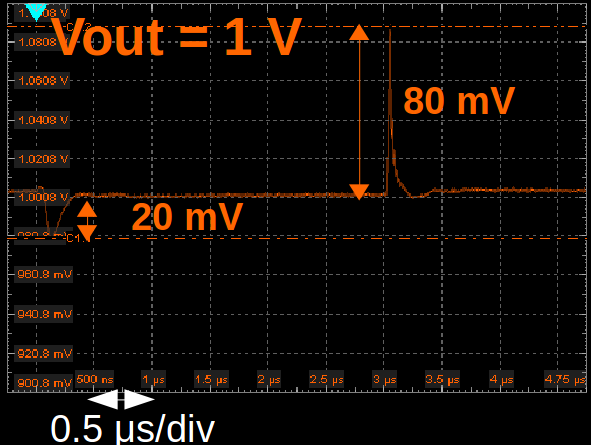
\includegraphics[width=.95\linewidth]{Immagini/zoomTransientTest2}
  \caption{ }
  \label{TransientTest:sfig2}
\end{subfigure}
\begin{subfigure}{\textwidth}
  \centering
  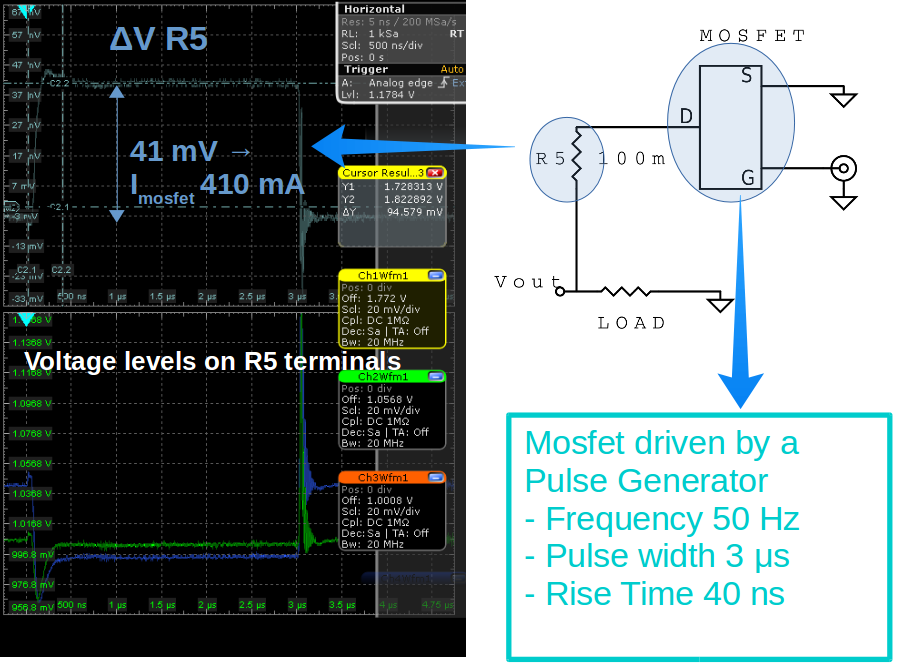
\includegraphics[width=0.9\linewidth]{Immagini/zoomTransientTest3bis}
  \caption{ }
  \label{TransientTest:sfig3}
\end{subfigure}
\caption{Schermata catturata dall'oscilloscopio: in giallo è rappresentata la tensione in ingresso, in arancione quella in uscita e in verde e blu la tensione sui i terminali di R5, la cui differenza è riportata in  azzurro. Nella sottofigura~\ref{TransientTest:sfig3}, a lato della schermata dell'oscilloscopio, è riportato lo schematico della parte di circuito con mosfet e resistenza.}
\label{TransientTest}
\end{figure}

Prendendo come riferimento la figura \ref{TransientTest}, si può notare un'asimmetria nelle variazioni di $\mathrm{V_{out}}$, in arancione in alto a destra.%, mentre in $\mathrm{V_{in}}$, in giallo in alto a sinistra, la risposta è simmetrica.
Allo stesso modo nella sottofigura~\ref{TransientTest:sfig3} in azzurro, è riportata la differenza tra le tensioni misurate ai capi di R5, riportate in basso con colore blu e verde e in cui si vede un'asimmetria in risposta al fronte di salita e discesa dell'impulso applicato al Gate del mosfet. 
Inoltre, sono visibili delle oscillazioni in corrispondenza dell'istante in cui il mosfet si spegne, sia sulle tensioni riferite a R5 sia sul $\mathrm{V_{out}}$.
%Questo comportamento si riflette su $\mathrm{V_{out}}$ ed è quindi all'origine dell'asimmetria.
Prima di procedere con misure dinamiche nelle varie combinazioni $\mathrm{I_{mosfet}}$--$\mathrm{R_{load}}$ si è cercato di capire l'origine delle asimmetria, in particolare se fosse collegata alla risposta del mosfet all'impulso.
L'impulso utilizzato in questa prima fase ha:
\begin{itemize}
  \item frequenza di 50Hz;
  \item durata di 3 $\mu$s;
  \item fronte di salita di 40 ns.
\end{itemize}
%In questa prima fase l'impulso utilizzato ha le seguenti caratteristiche: frequenza 50 Hz, durata 3 $\mu$s, durata del fronte di salita 40 ns.

\subsubsection{Contributo mosfet}
\begin{figure}
\centering
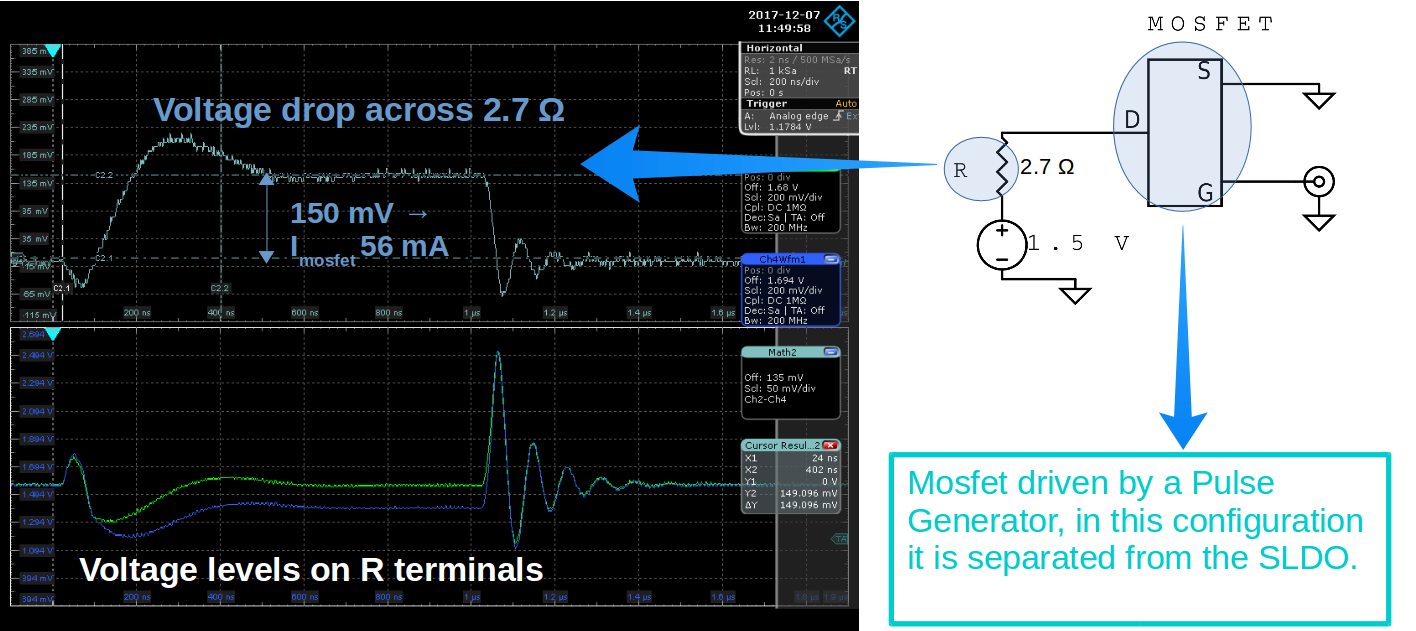
\includegraphics[width=\linewidth]{Immagini/MosfetBehaviourbis}
\caption{Sulla sinistra è riportato la schermata dell'oscilloscopio, che mostra l'andamento della tensione sui terminali di R in funzione del tempo, sulla destra è invece riportato lo schema della modifica al circuito.}
\label{MosfetBehaviour}
\end{figure}

\begin{figure}
\centering
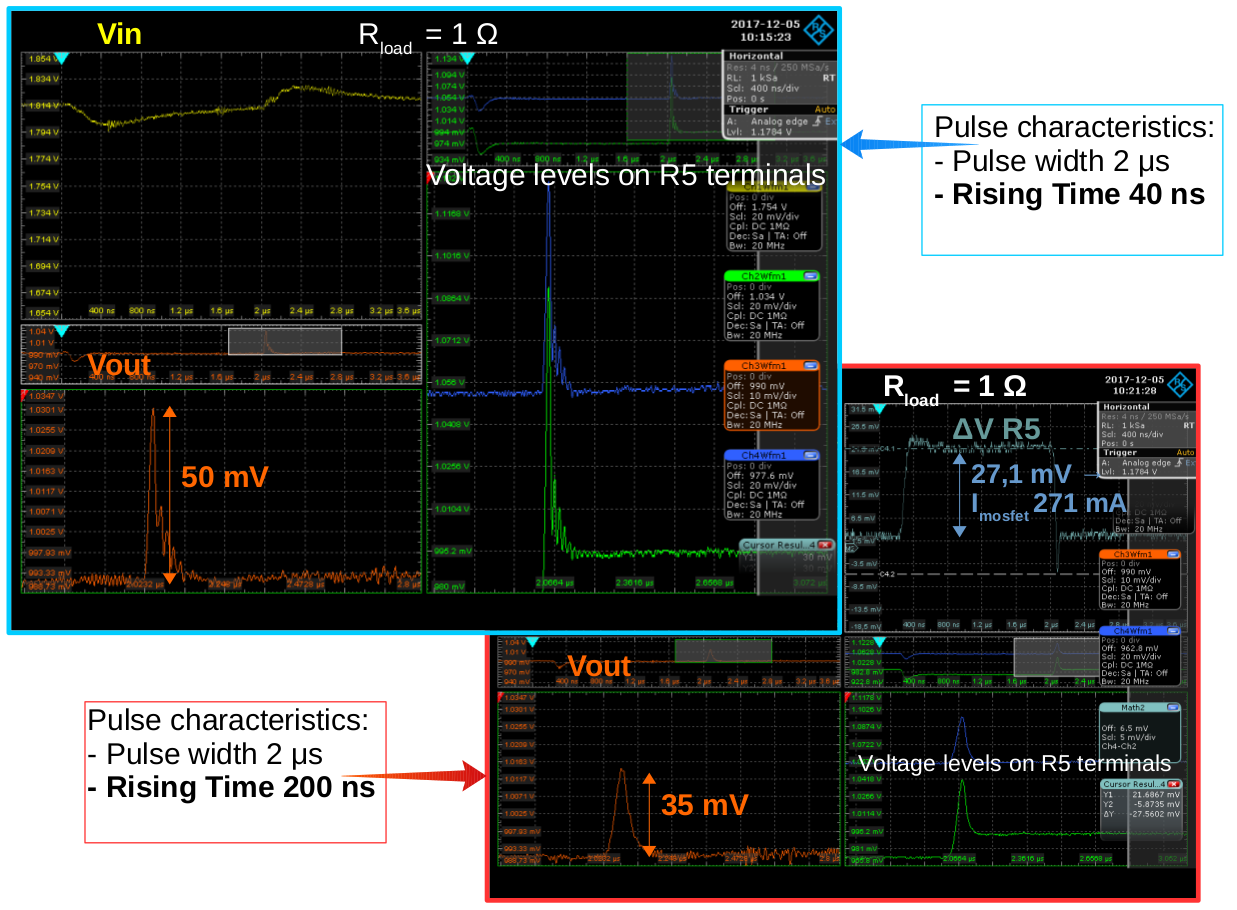
\includegraphics[width=\linewidth]{Immagini/RiseTime}
\caption{In alto a sinistra è riportata la risposta del $\mathrm{V_{out}}$ per impulsi con tempo di salita 40 ns, il basso a destra invece è la risposta a impulsi con tempi di salita di 200ns. Sia per il $\mathrm{V_{out}}$ che per le tensioni su R5 il comportamento migliora rallentando l'impulso.}
\label{RiseTime}
\end{figure}

Per esaminare il comportamento del mosfet in risposta all'impulso mandato sul Gate, si è proceduto ad isolare questa parte del circuito dal resto della scheda di test, connettendo al Drain una resistenza in serie ad una batteria stilo, al posto della connessione con il $\mathrm{V_{out}}$ dello ShuntLDO.
La batteria ricopre il ruolo di $\mathrm{V_{out}}$, mentre la resistenza è necessaria alla misura delle correnti che scorrono nel mosfet ed ha un valore di 2.7 $\Omega$. 


Come si vede dalla figura \ref{MosfetBehaviour}, le oscillazioni in corrispondenza dello spegnimento del mosfet sono presenti anche una volta che questo è stato isolato.
Questo comportamento è segno del fatto che queste oscillazioni sono generate dal mosfet stesso nel momento in cui il canale, che collega Drain e Source, si interrompe.
Inoltre, il fronte di salita è circa $100 \ns$, più lungo di quello dell'impulso, indice del fatto che il mosfet ha una risposta più lenta. %e non $40 \ns$ come ci aspetteremmo da un mosfet ideale con risposta istantanea.
Esaminando la documentazione del mosfet~\cite{MOSFET} presente sulla scheda di test 
%footnote{ZXMN20B28KTC http://www.mouser.com/ds/2/115/ZXMN20B28K-94822.pdf
si può verificare che effettivamente il tempo di ``accensione'' è superiore a $40 \ns$ (\textit{Turn-on rise time} $76.9 \ns$) e, inoltre, sono presenti capacità in ingresso equivalenti a $\mathrm{358 pF}$.
La risposta dello ShuntLDO è quindi mascherata per segnali più veloci della risposta del mosfet, per questo motivo le misure successive sono state effettuate utilizzando un tempo di salita del segnale del generatore di impulsi di $200 \ns$.
La figura \ref{RiseTime} mostra il miglioramento fra la configurazione con tempo di salita del generatore di $40 \ns$ e quella con $200 \ns$.
In questo modo si verifica la risposta dello ShuntLDO cad una variazione di carico più lenta, ma meno affetta dal mosfet.
%In figura \ref{RiseTime} è visibile come la situazione precedente, in cui l'impulso ha un tempo di salita di 40 ns, migliora visibilmente passando a 200 ns, in questo modo quello che viene simulato all'uscita dello ShuntLDO è un variazione di carico più lenta ma il cui comportamento è affetto in modo minore dalle caratteristiche del mosfet. 

\subsubsection{Misure}

Di seguito sono riportate le misure di caratterizzazione della tensione di ingresso, $\mathrm{V_{in}}$, e di uscita, $\mathrm{V_{out}}$, per tre differenti valori di $\mathrm{R_{load}}$ e al variare di $\mathrm{I_{mosfet}}$.
I valori di $\mathrm{R_{load}}$ scelti sono: $1 \Ohm$, $2.1 \Ohm$ e $4 \Ohm$; dato che $\mathrm{V_{out}=1 \V}$, in termini di correnti  $\mathrm{I_{load}}$, questi corrispondono rispettivamente a $1 \A$, $0.475 \A$ e $0.250 \A$.
%Oltre alla misura delle variazioni in ampiezza di $\mathrm{V_{in}}$ e $\mathrm{V_{out}}$ sono stati misurati anche i tempi di  recupero delle stesse.

\`E interessante notare che il tempo di recupero di $\mathrm{V_{in}}$ e $\mathrm{V_{out}}$ differiscono notevolmente: il primo è molto più lungo, dell'ordine dei $\mu$s, e dipendente dal valore di $\mathrm{I_{mosfet}}$, il secondo ha durata di circa $300 \ns$ indipendentemente dal valore di $\mathrm{I_{mosfet}}$.
Questo comportamento è imputabile al fatto che il riequilibrio della tensione di ingresso dipende anche dal generatore esterno, le cui variazioni sono più lente.
Va ricordato che lo ShuntLDO è alimentato in corrente con $1.5 \A$, dunque nel momento in cui $\mathrm{I_{load}+I_{mosfet}}$ raggiungono valori vicini o addirittura superiori  a $\mathrm{I_{in}}$, si ha un crollo della tensione in ingresso e del $\mathrm{V_{out}}$, poiché si sta chiedendo allo ShuntLDO di fornire una corrente superiore a quella a sua disposizione.

Per ciascun valore di $\mathrm{R_{load}}$, dunque, è stata fatta variare la corrente assorbita dal mosfet $\mathrm{I_{mosfet}}$ e misurato l'effetto di undershoot e overshoot sulle tensioni di $\mathrm{V_{out}}$ e $\mathrm{V_{in}}$. 
% Con corrente totale si intende la somma di quella assorbita dal mosfet e dalla resistenza di carico.
Le misure eseguite prendono in considerazione anche situazioni in cui la variazione del consumo in corrente eccede l'intervallo fisico di operatività del chip. Misure in cui la variazione del carico è il doppio del valore statico hanno interesse nell'ottica di quello che può succedere al momento dell'accensione del ROC.%, le cui variazioni di consumo in regime di lavoro, di norma, non superano i 500 mA.(controllare) 
Come detto in precedenza, gli impulsi utilizzati presentano una durata che consente di differenziare tra gli effetti dovuti al fronte di salita e quelli prodotti dal fronte di discesa. 
Facendo riferimento alla figura \ref{VoutUnd}, si possono vedere, in valore assoluto,gli undershoot della tensione di uscita a cui è applicato il carico in funzione della corrente che scorre nel mosfet (sinistra) e della corrente totale (destra), dove questa è la somma di quella assorbita dal carico e quella del mosfet. 
%I primi risultati riportano gli undershoot della tensione di uscita a cui è applicato il carico, riferendosi ai grafici in figura \ref{VoutUnd} sono riportati i valori assoluti di tali variazioni in funzione della corrente che scorre nel mosfet (sinistra) e della corrente totale (destra), la corrente totale è somma di quella assorbita dal carico e dal mosfet. 
\begin{figure}
\centering
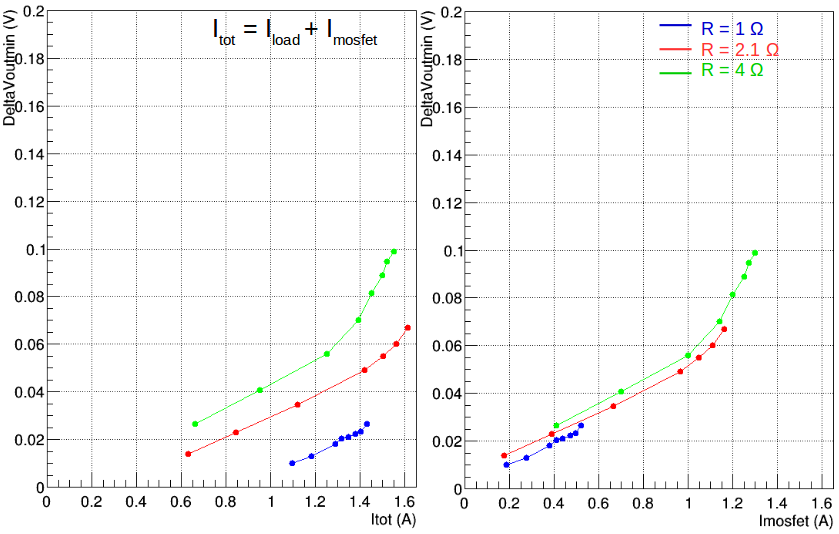
\includegraphics[width=0.9\linewidth]{Immagini/VoutUnd}
\caption{Grafici che riportano l'entità dell'undershoot del $\mathrm{V_{out}}$ in funzione della corrente totale, grafico di sinistra, e della corrente del mosfet, grafico di destra.}
\label{VoutUnd}
\end{figure}
\begin{figure}
\centering
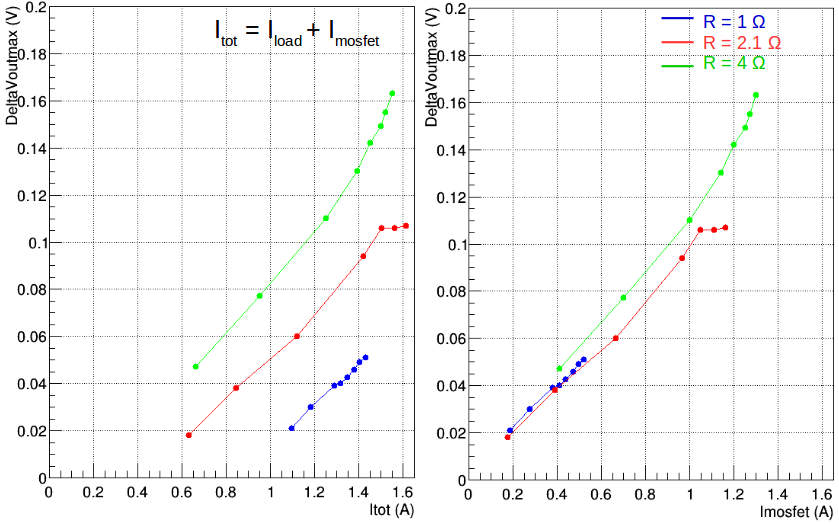
\includegraphics[width=0.9\linewidth]{Immagini/VoutOver}
\caption{Grafici che riportano l'entità dell'overshoot del $\mathrm{V_{out}}$ in funzione della corrente totale, grafico di sinistra, e della corrente del mosfet, grafico di destra.}
\label{VoutOver}
\end{figure}
In blu sono riportate le misure ottenute con un carico resistivo di $1 \Ohm$, in rosso $2.1 \Ohm$  e in verde $4 \Ohm$.
Come si può vedere dal grafico di destra, le tre curve seguono lo stesso andamento, dato che vi è una relazione fra la variazione di $\mathrm{V_{out}}$ e $\mathrm{I_{mosfet}}$, indipendente dal valore della resistenza.
Inoltre, limitandosi ad un intervallo di variazioni di corrente verosimili per il ROC, si osservano variazioni relativamente piccole di $\mathrm{V_{out}}$.
Ad esempio, con $\mathrm{I_{mosfet}= 0.4 \A}$, $\mathrm{\Delta V_{out} \simeq 20\mV}$.
Lo stesso comportamento è visibile nei grafici di figura \ref{VoutOver}, dove è riportata l'entità delle variazioni di $\mathrm{V_{out}}$ a seguito dello spegnimento del mosfet, cioè l'effetto che si ha sul fronte di discesa dell'impulso. 
%Nell'esaminare questi andamenti va ricordato che la corrente in ingresso al circuito è 1.5 A, quindi punti per i quali si ha una $\mathrm{I_{tot}}$ vicina o superiore a questo valore sono ottenuti in una situazione in cui lo ShuntLDO è impossibilitato a compiere il suo lavoro. 
%Ricordiamo che la corrente che passa in $R_3$ è un millesimo di quella che scorre nel ramo in cui si hanno carico e shunt.

Come per il $\mathrm{V_{out}}$ è stato misurato l'undershoot e l'overshoot della tensione in ingresso $\mathrm{V_{in}}$. I grafici degli undershoot sono riportati in figura \ref{VinUnd}, quelli riguardanti gli overshoot in figura \ref{VinOver}. 

\begin{figure}
\centering
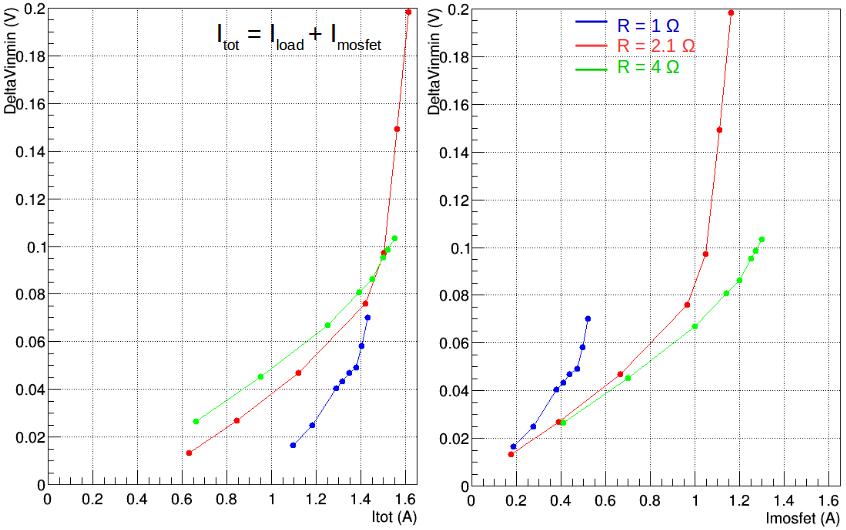
\includegraphics[width=0.9\linewidth]{Immagini/VinUnd}
\caption{Grafici che riportano l'entità dell'undershoot del $\mathrm{V_{in}}$ in funzione della corrente totale, grafico di sinistra, e della corrente del mosfet, grafico di destra.}
\label{VinUnd}
\end{figure}

\begin{figure}
\centering
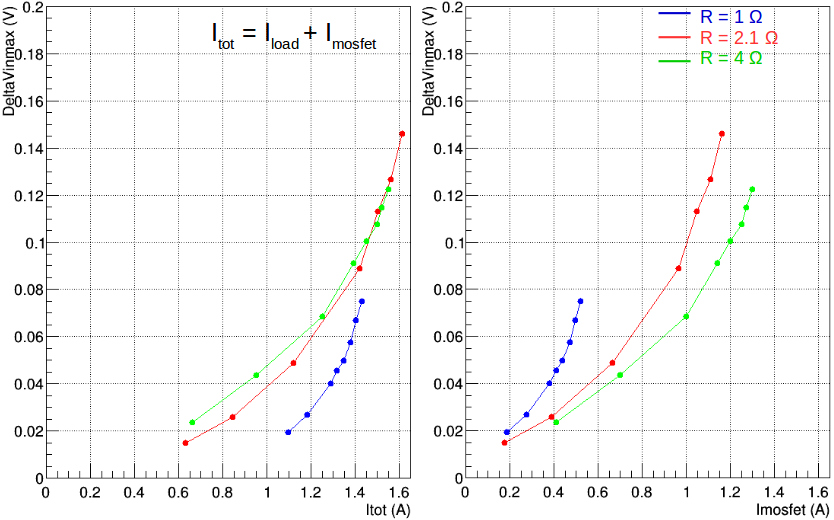
\includegraphics[width=0.9\linewidth]{Immagini/VinOver}
\caption{Grafici che riportano l'entità dell'undershoot del $\mathrm{V_{in}}$ in funzione della corrente totale, grafico di sinistra, e della corrente del mosfet, grafico di destra.}
\label{VinOver}
\end{figure}

In entrambi i casi la variazione della tensione in ingresso dipende sia dalla variazione di corrente $\mathrm{I_{mosfet}}$ che dalla corrente fissa $\mathrm{I_{load}}$. 
Per valori elevati di $\mathrm{I_{mosfet}}$ la tensione in ingresso inizia ad oscillare, con periodi di qualche $\mu$s.
Questo comportamento è dovuto al generatore utilizzato, in particolare l'alimentazione in corrente è stata ottenuta utilizzando un generatore di tensione, ma limitando la corrente in uscita. 
Nel momento in cui si ha una variazione di carico molto veloce che provoca un abbassamento di $\mathrm{V_{out}}$, si ha una piccola ripercussione sulla tensione di ingresso: dato che il generatore è di tensione, limitato in corrente, per tenere costante $\mathrm{I_{in}}$ avrà un abbassamento di tensione, ma con tempi più lunghi rispetto a quelli con cui lo ShuntLDO riesce a riequilibrare $\mathrm{V_{out}}$.
Il comportamento oscillatorio di $\mathrm{V_{in}}$, che compare quando $\mathrm{I_{tot}}$ è intorno al valore massimo, $\mathrm{I_{in}}$, ha permesso di constatare come fluttuazioni della tensione in ingresso non influiscano sulla tensione generata dal regolatore.
Questo può essere visto utilizzando l'oscilloscopio: in Fig.\ref{DipVoutVin} è mostrata una schermata dell'oscilloscopio in cui è riportato, in giallo, l'andamento di $\mathrm{V_{in}}$ in funzione del tempo, e, in arancione, la tensione di $\mathrm{V_{out}}$.
Si nota che le scale di tempo di recupero sono differenti, i.e. alcuni $\mu$s per $\mathrm{V_{in}}$ e circa $300 \ns$ per $\mathrm{V_{out}}$.

\begin{figure}
\begin{subfigure}{.5\textwidth}
  \centering
  \includegraphics[width=.95\linewidth]{Immagini/zoomDipendenzaVoutdaVin1}
  \caption{1a}
  \label{DipVoutVin:sfig1}
\end{subfigure}%
\begin{subfigure}{.5\textwidth}
  \centering
  \includegraphics[width=.95\linewidth]{Immagini/zoomDipendenzaVoutdaVin2}
  \caption{1b}
  \label{DipVoutVin:sfig2}
\end{subfigure}
\caption{Differenze nei tempi di recupero tra $\mathrm{V_{out}}$, in giallo, e $\mathrm{V_{out}}$, in arancione.}
\label{DipVoutVin}
\end{figure}
%\begin{figure}
%\centering
%\includegraphics[scale=.35]{Immagini/DipendenzaVoutdaVin}
%\caption{Differenze nei tempi di recupero tra $\mathrm{V_{out}}$, in giallo, e $\mathrm{V_{out}}$, in arancione.}
%\label{DipVoutVin}
%\end{figure}

\subsubsection{Serie di due ShuntLDO}

Dato che eventuali oscillazioni della tensione in ingresso causerebbero oscillazioni di tensione in tutta la catena di moduli, è importante che queste non si ripercuotano sul $\mathrm{V_{out}}$. 
Per verificare questo aspetto si è misurato con l'oscilloscopio la tensione di uscita di uno ShuntLDO messo in serie ad un secondo a cui è applicato un carico variabile, tramite l'utilizzo del mosfet, come già visto nelle misure precedenti.
In figura \ref{SLDOserie} sono affiancati uno schema del setup (sinistra) e la foto dei due ShuntLDO in serie (destra). 
Il serie di due ShuntLDO, entrambi con un carico statico di $4 \Ohm$, è alimentato con una corrente in ingresso di $1.5 \A$ e sul secondo ShuntLDO è collegato l'impulsatore che regola l'assorbimento di corrente  da parte del mosfet. 
Acquisendo con l'oscilloscopio la tensione di $\mathrm{V_{out}}$ di entrambi e il $\mathrm{V_{in}}$ del primo ShuntLDO della catena (quello con il solo carico statico) è stato possibile verificare come le fluttuazioni di tensione non influenzino la generazione della tensione di $\mathrm{V_{out}}$.
\begin{figure}[h!]
\centering
\includegraphics[scale=.30]{Immagini/SLDOserie}
\caption{Sulla destra foto dei due ShuntLDO in serie di cui a sinistra è riportato uno schema delle connessioni con generatore e impulsatore.}
\label{SLDOserie}
\end{figure}
In particolare in Fig.~\ref{ScreenSerie} si vede che, nonostante il secondo ShuntLDO sia in una situazione estrema, la generazione di $\mathrm{V_{out}}$ da parte del primo non ha ripercussioni. 
Il campionamento dei segnali mostrati, acquisiti con l'oscilloscopio, è stato ottenuto con una $\mathrm{I_{mosfet}}$ di $1.2 \A$, corrispondenti ad una $\mathrm{I_{tot}}$ di circa $1.45 \A$, quindi molto vicino al limite di $1.5 \A$. 
\begin{figure}[h!]
\centering
\includegraphics[scale=.32]{Immagini/ScreenSerie}
\caption{Schermata dell'oscilloscopio in cui è riportata in giallo la tensione in ingresso al primo ShuntLDO della catena,  in celeste la tensione di $\mathrm{V_{out}}$ sempre dello ShuntLDO1 e in verde la tensione di $\mathrm{V_{out}}$ dello ShuntLDO2 su cui è applicato il carico dinamico. Le fluttuazioni in tensione originate dalla variazione di carico sullo ShuntLDO2 si ripercuotono sul $\mathrm{V_{in}}$ dello ShuntLDO1 (giallo) ma non sulla tensione da esso generata (celeste).}
\label{ScreenSerie}
\end{figure}
In verde è riportato l'andamento di $\mathrm{V_{out}}$ del secondo ShuntLDO, che mostra importanti undershoot e overshoot, i quali, a loro volta e come visto in precedenza, causano come visto in precedenza, fluttuazioni della tensione in ingresso. 
La tensione di ingresso dello ShuntLDO2 corrisponde alla terra della scheda di test su cui si trova lo ShuntLDO1.
Le visibili fluttuazioni di questa, quindi, si ripercuotono su ShuntLDO2.
Nonostante ciò, come risultato importante, si può notare che $\mathrm{V_{out}}$ del primo ShuntLDO sia indipendente da queste.

\chapter{Il ROC prototipo RD53A}
\label{cap:RD53A}

Lo sviluppo di un sistema di alimentazione seriale e del circuito di alimentazione ShuntLDO, che gestisce localmente le tensioni, è parte integrante del ROC che viene sviluppato nell'ambito della collaborazione RD53~\cite{RD53} e, in particolare, del primo prototipo messo a punto dalla collaborazione, RD53A~\cite{RD53A}, che \`e diventato disponibile per la comunit\`a scientifica alla fine del 2017.

Questo prototipo costituisce una pietra miliare molto importante per il progetto dei rivelatori a pixel per HL-LHC \`e sar\`a utilizzato non solo per validare le scelte strettamente relative al ROC stesso (resistenza alla radiazione e prestazioni rispetto ai requisiti di HL-LHC), ma anche per finalizzare lo sviluppo dei sensori e del resto dell'apparato.
%, e quindi la tolleranza al danneggiamento da radiazioni, soglie di lavoro basse e stabili nel tempo, capacità di gestire un alto flusso di particelle incidenti e l'utilizzo di trigger veloci.

\section{Organizzazione di RD53A, alimentazione e Front End}
\label{Organizzazionechip}


\begin{figure}
\centering
\includegraphics[width=0.75\textwidth]{Immagini/RD53ALayout}
\caption{La geometria reale di RD53A: il ROC è largo $20\mm \times 11.8\mm$ con una pixel matrix di $400\times 192$ pixel corrispondenti ad un'area attiva di $20\mm \times 9.6\mm$.}
\label{RD53ALayout}
\end{figure}
\begin{figure}
\centering
\includegraphics[width=0.75\textwidth]{Immagini/AnalogIsland}
\caption{Disegno ricavato dalle maschere di RD53A dove sono visibili le `isole analogiche' dei \textit{front end} della `pixel matrix' circondate dal `mare' della circuiteria digitale.}
\label{AnalogIsland}
\end{figure} 
Facendo riferimento alla Fig.~\ref{RD53ALayout}, l'area del ROC che sarà saldata col sensore tramite bump bonding, detta anche {\em pixel matrix}, è posta nella parte alta ed è organizzata in una matrice di $192\times400$ pixel di area $50\um \times 50 \um$ per un'area totale di $20\mm \times 9.6\mm$.
Al di sopra di questa è presente una fila di piazzole a scopo diagnostico che sarà eliminata nella versione finale.

La matrice di pixel è organizzata in \textit{cores} di 8$\times$8 pixel, all'interno di ciascuno i 64 circuiti di preamplificazione (front end) sono disposti in regioni di 4, chiamati {\em isole analogiche}, come mostrato in Fig.~\ref{AnalogIsland}. 
Data la miniaturizzazione necessaria, l'area del ROC deve essere completamente sfruttata e, per questo, le isole analogiche sono circondate da un `mare' di circuiteria digitale. 


\begin{figure}
\centering
\includegraphics[width=0.8\textwidth]{Immagini/RD53Apianofunzionale}
\caption{Il piano funzionale di RD53A in cui, nella parte bassa, sono visibili, in particolare, le piazzole di potenza dello ShuntLDO.}
\label{RD53AFunct}
\end{figure}
Come rappresentato nel piano funzionale in Fig.~\ref{RD53AFunct}, al di sotto delle pixel matrix \`e collocata la regione detta `periferia' che, oltre alle piazzole di microsaldatura per la connessione del ROC, ospita tutti gli altri blocchi funzionali: l'{\em Analog Chip Bottom} (ACB) ospita i blocchi analogici (DAC, ADC, sensori di temperatura...); il {\em Digital Chip Bottom} (DCB) raggruppa i blocchi digitali per la gestione dell'Input/Output e della configurazione. Tenendo conto della periferia la dimensione totale del ROC \`e $20\mm \times 11.8\mm$.

L'alimentazione di RD53A \`e dimensionata su un numero di pixel doppio rispetto a quelli effettivamente presenti, comparabile per\`o con quello che sar\`a il ROC finale di superficie circa doppia. RD53A sar\`a normalmente alimentato tramite un'unica linea di alimentazione seriale che servirà due ShuntLDO, uno che fornisce VDDD (la tensione di alimentazione della parte digitale) e uno che fornisce VDDA (la tensione di alimentazione della parte analogica). Essendo un prototipo \`e anche possibile alimentare direttamente le linee VDDD e VDDA scavalcando la regolazione.
Come accennato in precedenza, la parte dello ShuntLDO in cui viene dissipata molta potenza (il mosfet di shunt M4) \`e distribuita in quattro `piazzole di potenza' per ciascun regolatore, ospitate nella periferia (come visibile in~Fig.~\ref{RD53AFunct}). Solo una di queste contiene la parte comune di controllo dello ShuntLDO. Questo accorgimento permette di distribuire la dissipazione di calore dovuta allo shunt conferendo una maggiore affidabilità. Ciascuna piazzola \`e stata dimensionata in base al previsto consumo totale del ROC finale, ovvero per una corrente massima di $500\mA$ per un totale di $4.0\A$ per l'intero ROC, tenendo conto sia della parte digitale che analogica.

%\section{Front End}

Dato che RD53A non deve essere inteso come il prodotto finale, ma come un prototipo in cui coesistono varie possibili linee di sviluppo, al suo interno sono presenti tre differenti tipologie di circuiti di preamplificazione di front end (FE) per permettere un confronto in termini di prestazioni.
% possiede molte modifiche di design utili solo in una prima fase di test, ad esempio al suo interno sono presenti tre diversi front end (FE), già questo causa una non uniformità del chip. 
La pixel matrix \`e suddivisa equamente tra i FE Sincrono, Lineare e Differenziale come visibile in Fig.~\ref{FrontEnd}. 
%Questi tre circuiti sono stati progettati da tre differenti gruppi e tra di loro ci sono importanti differenze.

Il FE Sincrono sfrutta un sistema di \textit{auto-zeroing} della linea di base, campionandola periodicamente, invece di aggiustare la soglia pixel per pixel. 
Il FE Lineare utilizza un amplificatore lineare all'ingresso del comparatore, che confronta il segnale con la soglia impostata. 
Il FE Differenziale ha uno stadio di guadagno differenziale all'ingresso del discriminatore. % e sbilanciando i due canali implementa la soglia.

In comune ai tre FE, invece, abbiamo la rete di polarizzazione per il sensore ed il circuito per iniettare segnali di calibrazione. Indipendentemente dall'implementazione ciascun canale di lettura \`e caratterizzato da una certa soglia, normalmente espressa in carica equivalente, oltre la quale il segnale di particella viene digitalizzato e letto. La soglia deve essere accuratamente calibrata: se \`e troppo alta si possono avere inefficienze; se troppo bassa una fluttuazione di rumore pu\`o essere confusa con un segnale di particella.

%Questi ultimi due permettono un miglior confronto fra le prestazioni dei FE.
%Inoltre, i tre FE condividono l'area del sensore e, dato che la matrice è larga 400 pixel ed è suddivisa in core da 8 $\times$ 8 pixel, non è possibile avere una egual area per i tre, ma due avranno 17 core per riga ed uno solo 16.
%I FE Lineare e Differenziale sono stati posti accanto in quanto hanno funzionalità simili e metterli vicino consente di avere un'area con una risposta più uniforme anche in termini di consumi. 
\begin{figure}
\centering
\includegraphics[scale=.3]{Immagini/FrontEnd}
\caption{Disposizione dei tre differenti front end rispetto alla matrice di pixel.}
\label{FrontEnd}
\end{figure}

% Descriviamo ora brevemente il funzionamento di ciascuno dei tre Front End:

% \begin{itemize}

% \begin{figure}
% \centering
% \includegraphics[width=\textwidth]{Immagini/SchemaSincrono}
% \caption{Schema semplificato del \textit{front end} Sincrono.}
% \label{SchemaSincrono}
% \end{figure}
% \item \textbf{Sincrono}. Il FE Sincrono, il cui schema è visibile in Fig.~\ref{SchemaSincrono}, \`e costituito da un amplificatore di carica (\textit{Charge Sensitive Amplifier} o CSA) a stadio singolo con un Krummenacher feedback accoppiato in AC ad un discriminatore sincrono, formato da un amplificatore differenziale e un latch di feedback positivo. 
% Il Krummenacher feedback è progettato in modo da compensare sia la corrente di buio del sensore sia la corrente di scarica della capacità presente nell'anello di reazione. 
% Maggiore la corrente maggiore la velocità con cui il segnale del preamplificatore torna al valore di \textit{baseline}.
% %Si tenga presente, come riferimento, che una carica di 10k$e^{-}$ e che produce un segnale di $10\nA$ di corrente e $400\ns$ di durata viene ridotta ad un segnale di $40\nA$ di corrente di $100\ns$.   
% %Per avere due differenti valori di guadagno, ci sono due capacità, rispettivamente di 2.5 fF e 4 fF. 
% A causa dei limiti della tecnologia a $65\nm$, si hanno fluttuazioni della \textit{baseline} in uscita dal primo stadio dell'ordine delle decine di millivolt tra un canale e l'altro e questa \`e la ragione dell'accoppiamento in AC del discriminatore. 
% In ogni caso le differenze tra transistor si traducono in un offset della tensione in uscita dal discriminatore tra i vari pixel. 
% Questo effetto, normalmente, è compensato con DAC locali che permettono regolazioni fini. 
% Nel FE Sincrono, invece, l'offset è compensato attraverso un meccanismo di auto azzeramento (\textit{auto zeroing}). 
% Per fare ciò è necessaria l'acquisizione del livello di tensione della \textit{baseline} ogni $100\us$s o meno.
% Durante le collisioni, la differenza tra segnale e baseline è inviata ad uno stadio di confronto che genera il segnale di uscita del discriminatore.

% \begin{figure}
% \centering
% \includegraphics[width=\textwidth]{Immagini/SchemaLineare}
% \caption{Schema semplificato del \textit{front end} Lineare.}
% \label{SchemaLineare}
% \end{figure}
% \item \textbf{Lineare}. Lo schema semplificato del 
% Il FE Lineare è mostrato in Fig.~\ref{SchemaLineare}. Il circuito di lettura include un amplificatore di carica con un Krummenacher feedback per far fronte all'aumento di corrente di dispersione indotta dagli alti livelli di radiazione attesa. 
% La scelta di un amplificatore a stadio singolo è dettata dai limiti sui consumi e sullo spazio disponibile all'interno del chip. 
% Il segnale ottenuto dall'amplificatore di carica è mandato ad un comparatore che, insieme al contatore ToT (\textit{Time over Threshold}), è utilizzato per fare la conversione a segnale digitale. 
% Gli aggiustamenti della tensione di soglia sono gestiti, canale per canale, da un circuito locale basato su un \textit{binary weighted} DAC, a 4 bit, che genera una corrente $\mathrm{I_{DAC}}$, fornendo una regolazione locale della soglia. 
% Questo tipo di front end è stato ottimizzato per una carica massima di 30000 elettroni e un consumo complessivo di circa 4 $\mu$A. 
% L'amplificatore può essere utilizzato in regime di alto o basso guadagno, modificando il bit GAIN$\_$SEL, mentre la corrente di recupero, $\mathrm{I_K}$/2, proveniente dal circuito di Krummenacher feedback, può essere configurata tramite un DAC. 
% In configurazione di alto guadagno, per un segnale di carica pari a 30000, elettroni si ha un ToT di circa 400 ns, risultante in una corrente $\mathrm{I_K}$ di 25 nA. 
% La risoluzione attesa è di 15 mV/k$e^{-}$, mentre diventa di 7.5 mV/k$e^{-}$ in configurazione di basso guadagno. 
% Le prestazioni del preamplificatore di carica sono determinate, principalmente, dall'ingresso dell'amplificatore di carica e dalla parte del circuito di feedback con transistor PMOS. Dalle simulazioni il rumore in carica equivalente, per un rivelatore con capacità di 50 fF, è di 87 elettroni e, dopo la messa a punto, la dispersione della soglia scende da 380 a 35 elettroni.
% %Da simulazioni la dispersione della soglia dovrebbe passare da 380 elettroni a 35 elettroni dopo la messa a punto.

% \begin{figure}
% \centering
% \includegraphics[scale=.3]{Immagini/SchemaDifferenziale}
% \caption{Schema semplificato del \textit{front end} Differenziale.}
% \label{SchemaDifferenziale}
% \end{figure}
% \item \textbf{Differenziale}. Il front end Differenziale è un circuito puramente analogico: non ha al suo interno latches, flip-flop o contatori. 
% I valori di configurazione sono, però, forniti da un nucleo digitale, che riceve dalla parte analogica solo il segnale in uscita del comparatore. 
% Naturalmente è necessaria la presenza di un ADC per la digitalizzazione del ToT ottenuto dal comparatore, anch'esso implementato interamente nella parte digitale. 
% Lo schema a blocchi del front end differenziale è riportato in figura \ref{SchemaDifferenziale}. 
% Il pre amplificatore, presente nel primo stadio, ha un guadagno continuo, regolabile tra i due valori di capacità presenti nell'anello di reazione.
% Il feedback in corrente è impostabile globalmente e non può essere regolato su ogni singolo pixel. 
% Dalle misure sui prototipi è stato visto che la dispersione nei valori di ToT che ne consegue ha un livello accettabile anche senza la necessità di una pre regolazione.  
% In caso di assenza di segnale, il feedback assicura che input e output del preamplificatore siano allo stesso potenziale.
% Nel secondo stadio, il pre comparatore fornisce un guadagno aggiuntivo e agisce come soglia differenziale.
% La soglia globale può essere regolata tramite le tensioni VTH1 e VTH2, mentre localmente la soglia è modificata utilizzando un \textit{resistor ladder} a 4 bit in ciascuno dei due rami del pre comparatore.
% Oltre ai 4 bit ce n'è un quinto che seleziona il ramo da modificare. 
% Dopo il pre comparatore si ha uno stadio con un comparatore, la cui uscita è collegata alla regione digitale tramite porte logiche. 
% Progettato per operare con una soglia di 500 elettroni, la parte analogica ha un consumo di 4$\mu$A/pixel, considerando una capacità di 50 fF e 10 nA di corrente dispersa.

% \end{itemize}

\section{Lo ShuntLDO di RD53A}
\begin{figure}
\centering
\includegraphics[width=\textwidth]{Immagini/SLDO_RD53A}
\caption{Regolatore LDO con Shunt (ShuntLDO) nella versione implementata in RD53A.}
\label{SLDO_RD53A}
\end{figure}
In RD53A l'alimentazione è gestita da due ShuntLDO, uno per la parte analogica ed uno per quella digitale, in cui la parte di potenza \`e distribuita nella periferia come descritto in precedenza. Rispetto al circuito ShuntLDO a $2\A$ descritto nella Sezione~\ref{ShuntLDO2A}, la tensione di offset $\mathrm{V_{ofs}}$ è generata con una circuiteria migliorata. Lo schema del circuito di ShuntLDO è riportato in Fig.~\ref{SLDO_RD53A}, mentre i pi\`u importanti parametri di funzionamento sono riportati in Tabella~\ref{tab:sldord53a}:

%\begin{center}
\begin{table}
\begin{small}
\noindent\setlength\tabcolsep{4pt}%
\begin{tabularx}{\linewidth}{c|c|c|c|c|X}
%\begin{tabular}{|c|c|c|c|c|l|}
%\hline
\textbf{Pin} & \textbf{Tipologia} & \textbf{Min} & \textbf{Tipico} & \textbf{Max} & \textbf{Descrizione} \\ \hline
$\Vin$ & Tensione & 1.4 V & & 2.0 V & Alimentazione esterna (in tensione)\\
 & Corrente & 0 A & 0.5 A & 2.0 A & Alimentazione esterna (in corrente)\\ \hline 
$\mathrm{V_{SHUNT}}$ & Tensione & 1.4 V & & 2.0 V & Alimentazione per il circuito di shunt; connesso a $\mathrm{\Vin}$\\ \hline% per operare con lo shunt, sconnesso in caso di alimentazione diretta\\ \hline
GND & Ground &  & &  & Riferimento locale e uscita della corrente di shunt\\ \hline
VDD & Tensione & 1.0 V & 1.2 V & 1.32 V & Tensione di uscita $\VDD$ del regolatore\\ \hline
$\mathrm{V_{ref}}$ & Analogico & 500 mV & 600 mV & 660 mV & Tensione di riferimento (VDD=2$\mathrm{V_{ref}}$)\\ \hline
$\mathrm{R_{INT}}$ & Analogico &  & $\mathrm{\Vin}$ &  & Connesso $\mathrm{\Vin}$ abilita la resistenza interna\\ \hline
$\mathrm{R_{EXT}}$ & Analogico & $300\Ohm$ &  &  & Terminale per una resistenza esterna da connettere a $\mathrm{\Vin}$\\ \hline
$\mathrm{I_{OFS}}$ & Analogico &  & $200\kOhm$ &  & Terminale per una resistenza esterna da connettere a GND per configurare $\mathrm{V_{ofs}}$ esternamente\\ \hline
$\mathrm{COMP_{ENB}}$ & Digitale &  & GND &  & A GND abilita il circuito di compensazione per capacità di uscita a bassa resistenza equivalente in serie ({\em ESR})\\
%\hline
\end{tabularx}
\end{small}
\caption{I terminali di configurazione e regolazione dello ShuntLDO di RD53A.}
\label{tab:sldord53a}
\end{table}
%\end{center}

Il valore di $\mathrm{V_{ofs}}$ è determinato tramite il terminale $\mathrm{I_{ofs}}$ previsto per connettervi un resistore $\mathrm{R_{iofs}}$ verso $\mathrm{GND}$ definendo cos\`i la tensione $\mathrm{V_{+A5}}$ all'ingresso non invertente di A5. La sorgente di corrente $\mathrm{I_{ofs}}$ fornisce $2\uA$ e quindi
\begin{equation}
\label{eq:V+a5}
\mathrm{V_{+A5} = 2 \uA \cdot R_{iofs}}
\end{equation}
tensione che viene poi raddoppiata sull'ingresso di A4 tramite il partitore R4/R5 sull'anello di reazione di A5. Ne consegue che:
\begin{equation}
\label{eq:Vofs}
\mathrm{V_{ofs} = 2\cdot 2\uA \cdot R_{iofs}}.
\end{equation}
%\begin{equation}
%\mathrm{V_{in}= 2 \cdot V_{iofs} + \dfrac{R3}{1000} \cdot I_{in}}
%\end{equation}
Le misure presentate nelle sezioni successive sono state ottenute con i seguenti valori di R3 e $\mathrm{R_{iofs}}$:
\begin{center}
\begin{tabular}{lc}
\hline
$\mathrm{R3}$ & $600\Ohm$ \\%misurata con il multimetro è 620
$\mathrm{R_{iofs}}$ & $250\kOhm$\\ 
\hline
\end{tabular}
\end{center}
Tale valore di $\mathrm{R_{iofs}}$ corrisponde a $\mathrm{V_{+A5}\simeq0.5\V}$ per cui, nell'andamento della tensione in ingresso in funzione della corrente, ci aspettiamo un $\mathrm{V_{ofs}\simeq 1\V}$.

Per quanto riguarda le tensioni di riferimento, come $\mathrm{V_{ref}}$, queste vengono generate all'interno del ROC da un circuito bandgap dedicato.
La tensione di riferimento del bandgap è configurabile a passi di circa $1\mV$ tramite un registro a 5 bit il cui valore di default \`e 16, corrispondente a una tensione di circa $1.15\V$ che varia leggermente da un ROC all'altro.
Un esempio è quello di Fig.~\ref{bandgap_trimming}, in cui sono riportati, per differenti ROC, gli andamenti misurati di $\mathrm{V_{ref}}$ al variare del valore impostato sul registro di configurazione. Per valori troppo piccoli di $\mathrm{V_{ref}}$ (che definiscono VDDA e VDDD) il ROC smette di funzionare e per questo motivo la parte sinistra del grafico non \`e popolata.
\begin{figure}
\centering
\includegraphics[width=0.85\textwidth]{Immagini/bandgap_trimming}
\caption{Andamento della tensione $\mathrm{V_{ref}}$ generata internamente, per due diversi ROC (per un totale di quattro bandgap), al variare del parametro di configurazione; il valore di default è 16. In due casi \`e riportata la retta di fit.}
\label{bandgap_trimming}
\end{figure}

\section{La Single Chip Card, scheda di test per RD53A}

Analogamente a quanto visto per gli ShuntLDO, che vengono collaudati usando una scheda di test, anche per il chip RD53A è necessaria una scheda di test detta \textit{Single Chip Card} (SCC) nella versione che ospita un solo ROC, visibile in~Fig.~\ref{fig:RD53onSCC}. 
\begin{figure}[t]
\centering
\includegraphics[width=0.5\textwidth]{Immagini/RD53onSCC.jpg}
\caption{Il prototipo di RD53A del gruppo di CMS di Firenze montato sulla sua SCC.}
\label{fig:RD53onSCC}
\end{figure}
Il ROC è fissato al centro di questa scheda e, attraverso microsaldature, è connesso ai vari elementi della scheda (terminali di monitoraggio, connettori di alimentazione, connettori con standard DisplayPort per la trasmissione/ricezione di dati, ponticelli/jumper di configurazione, ecc...). 
Ai bordi dell'apposito spazio in cui viene montato il ROC arrivano le varie piste da connettere, sotto vi è un generoso strato metallico collegato, tramite molti `via', al lato opposto della scheda e che assicura lo scambio termico consentendo, se necessario, l'applicazione di un sistema refrigerante o di un dissipatore sulla parte posteriore della SCC. 
Infatti, nel momento in cui l'alimentazione del ROC viene fornita dai due ShuntLDO, la corrente non utilizzata viene dissipata sui due shunt che si scaldano rendendo raccomandabile un minimo di raffreddamento per scongiurare danneggiamenti.
%La presenza di un raffreddamento è necessaria nel momento in cui l'alimentazione è data utilizzando i due ShuntLDO, infatti, la corrente non necessaria al chip viene dissipata sui due shunt che diventano punti molto caldi. 
%Al fine di evitare danneggiamenti del chip, e dell'eventuale sensore collegato, questo va raffreddato utilizzando dissipatori di calore. 

Dal momento che RD53A è un prototipo, si è lasciata la possibilità di configurare l'alimentazione esternamente, scegliendo tra tre diverse opzioni.
Inoltre, è possibile mantenere separate, a livello di alimentazione, la parte digitale e quella analogica, che nella versione finale di RD53A si prevede essere in parallelo. Le possibili configurazioni di alimentazione sono sotto elencate e in Fig.~\ref{SLDOmodes} sono riportati gli schemi di configurazione della SCC ad esse relativi.

\begin{description}
\item[Alimentazione con ShuntLDO] In questo caso il generatore utilizzato sarà in corrente. Per operare in configurazione ShuntLDO è necessario l'utilizzo di un sistema di raffreddamento per il ROC che, in normali condizioni di lavoro, può essere un semplice dissipatore passivo. Nella misura delle varie tensioni, però, l'effetto di deriva termica non è trascurabile e, quindi, per le future misure \`e in fase di preparazione un sistema di raffreddamento attivo che permetta di controllare le temperature.

\item[Alimentazione senza Shunt, con solo LDO] Questa configurazione necessita di un'alimentazione in tensione e sarà il generatore esterno a dover fornire più o meno corrente in relazione ai consumi del ROC. L'utilizzo del solo regolatore permette di avere un consumo ottimizzato in termini di potenza e, dunque, il ROC pu\`o essere utilizzato senza il bisogno di un sistema di raffreddamento.

\item[Alimentazione diretta] Lo ShuntLDO viene completamente escluso e il ROC è alimentato direttamente da un generatore di tensione esterno. L'alimentazione diretta deve essere utilizzata con particolare attenzione per evitare danneggiamenti del ROC. La presenza del regolatore LDO anche se privo di shunt, assicura che sbalzi di tensione all'ingresso dell'alimentazione non siano trasmessi al chip. Il regolatore, inoltre, tollera tensioni fino a $2 \V$, mentre RD53A già sopra $\sim 1.35\V$ rischia di danneggiarsi. L'esclusione di questa sicurezza con la scelta di utilizzare un'alimentazione diretta è, perciò, sconsigliata. 
\end{description}

\begin{figure}[h]
\centering
\includegraphics[width=0.30\textwidth]{Immagini/SLDOmode}
\hfill
\includegraphics[width=0.30\textwidth]{Immagini/LDOmodeDefault}
\hfill
\includegraphics[width=0.30\textwidth]{Immagini/DirectPowering}
\caption{Disposizione dei jumper per le varie configurazioni di alimentazione di RD53A. Sinistra: ShuntLDO. Centro: LDO senza la parte di shunt. Destra: alimentazione diretta. In tutti e tre i casi la stessa configurazione è usata per la parte analogica e la parte digitale.}
\label{SLDOmodes}
\end{figure}

\section{Caratterizzazione degli ShuntLDO su RD53A}
\label{MisureStaticheRD53A}

La caratterizzazione degli ShuntLDO di cui è dotato il ROC prototipo RD53A è stata effettuate inizialmente presso il CERN di Ginevra, nell'ambito delle attività congiunte tra la collaborazione RD53 e la collaborazione CMS, e poi presso l'INFN, Sezione di Firenze.

\subsection{Misure statiche}

Utilizzando la SCC in configurazione ShuntLDO, raffreddando il ROC in modo passivo con un radiatore a contatto termico con il retro della scheda di test, si è proceduto alla caratterizzazione statica del comportamento dei due circuiti di alimentazione presenti in RD53A, uno per la parte analogica e l'altro per quella digitale. 

Questo studio è stato effettuato con diverse configurazioni risultanti dalla combinazione di tre aspetti operativi:
%Nel far questo sono state scelte diverse configurazioni, le scelte principali possono essere riassunte in tre punti:
\begin{itemize}
  \item alimentazione dei due regolatori con ShuntLDO: indipendenti o in parallelo fra loro;
  \item rampa di corrente crescente o decrescente;
  \item tensioni di riferimento $\mathrm{V_{ref}}$ e $\mathrm{V_{+A5}}$: generate internamente o fornite dall'esterno.
%\item Tenere i due regolatori con ShuntLDO in parallelo o con alimentazione indipendenti.
%\item Variare la corrente partendo da 0 A incrementandola via via o partendo da 1.5 A andando poi a decrescere.
%\item Utilizzare $\mathrm{V_{ref}}$ e $\mathrm{V_{iofs}}$ generati internamente o fornirli esternamente.
\end{itemize}

In tabella~\ref{tab:legenda} è riportata la descrizione delle abbreviazioni utilizzate per le legende dei grafici.
\begin{table}
\begin{center}
%\noindent\setlength\tabcolsep{4pt}%
\begin{tabular}{l|l}
%\begin{tabularx}{\linewidth}{c|r}
%\multicolumn{2}{|c|}{Abbreviazione} & \multicolumn{1}{c|}{\multirow{2}{*}{Descrizione}}\\ 
 Abbreviazione & Descrizione\\ \hline
\multicolumn{2}{l}{Parte Analogica} \\
\hline
VINA & Tensione $\mathrm{V_{INA}}$ all'ingresso del regolatore  \\ \hline
VDDA & Tensione $\mathrm{V_{outA}}$ all'uscita del regolatore \\ \hline
$\mathrm{V_{iofs \_ m \_ A}}$ & $\mathrm{V_{+A5A}}$ \\ \hline   
$\mathrm{V_{ref \_ m \_ A}}$  & $\mathrm{V_{refA}}$ \\ \hline \hline  
\multicolumn{2}{l}{Parte Digitale} \\ \hline
% Abbreviazione & Descrizione\\ 
VIND & Tensione $\mathrm{V_{IND}}$ all'ingresso del regolatore  \\ \hline
VDDD & Tensione $\mathrm{V_{outD}}$ all'uscita del regolatore \\ \hline
$\mathrm{V_{iofs \_ m \_ D}}$ & $\mathrm{V_{+A5D}}$ \\ \hline   
$\mathrm{V_{ref \_ m \_ D}}$  & $\mathrm{V_{refD}}$ \\ 
\end{tabular}
\end{center}
\caption{Descrizione delle abbreviazioni utilizzate per le legende dei grafici.}
\label{tab:legenda}
\end{table}

\subsubsection{Alimentazioni indipendenti, rampa di corrente crescente, tensioni di riferimento interne}
\label{sec:iui}

\begin{figure}
\centering
\includegraphics[width=\textwidth]{Immagini/IUI2}
\caption{Grafici tensione-corrente ottenuti tenendo i due regolatori separati e variando le rispettive correnti $\mathrm{I_{in}}$ da $0\A$ a $1.5\A$.}%allungare descrivendo anche l'undershoot
\label{IUI}
\end{figure}
Le prime misure sono state eseguite utilizzando, come riferimento per $\mathrm{V_{out}}$ e $\mathrm{V_{iofs}}$, le tensioni generate internamente al ROC.
La corrente fornita ai due ShuntLDO, alimentati indipendentemente, è stata variata, contemporaneamente, da $0\A$ a $1.5\A$ a passi di $10\mA$.
L'andamento ottenuto è riportato in Fig.~\ref{IUI}.

La fluttuazione verso il basso ben visibile sulle tensioni della parte analogica, sia in ingresso che in uscita, è causata da uno sbilanciamento nella distribuzione delle correnti nei due ShuntLDO: quando si attiva la parte digitale si ha un picco di assorbimento di corrente a scapito della parte analogica che risulta nelle fluttuazioni qui riassunte:
\begin{center}
\begin{tabular}{ccc}
\hline
$\Delta \mathrm{V_{INA}}$ & $\Delta \mathrm{V_{refA}}$ &$\Delta \mathrm{V_{outA}}$  \\ \hline
$\sim$0.150 V & $\sim$ 0.030 V& $\sim$0.060 V\\ \hline     
\end{tabular}
\end{center}
Questo fenomeno è stato osservato nonostante la configurazione sia tale da avere i due ShuntLDO alimentati separatamente, segno che, all'interno del ROC, sono presenti fenomeni di `dialogo' fra i due ambiti: un po' di corrente scorre attraverso le connessioni tra le due regioni, causando la caduta di tensione osservate nella parte analogica.
%Questo avviene nonostante le alimentazioni dei due ShuntLDO siano separate, in quanto all'interno del chip ci sono zone di 'dialogo' tra regione analogica e digitale. 
%Si ha scorrimento di corrente attraverso connessioni tra le due regioni che causano cadute di tensioni nella parte analogica, questo comportamento è pericoloso e va evitato. 
Questo comportamento è potenzialmente dannoso perché può alterare la corretta sequenza di accensione con il rischio di fenomeni di oscillazione o che il ROC finisca in uno stato anomalo senza possibilità di recupero.

Inoltre, sempre dalla Fig.~\ref{IUI}, si può notare che $\mathrm{V_{outD}}$ sale parzialmente quando $\mathrm{I_{in}}$ raggiunge $\sim0.56\A$, non riuscendo però ad andare a regime, poiché la tensione $\mathrm{V_{IND}}$ non è ancora sufficientemente elevata da consentire una corretta regolazione. Questo, a sua volta, è dovuto al ritardo con cui $\mathrm{V_{+A5D}}$ raggiunge il valore corretto, solo per $\mathrm{I_{in}\sim 1.1\A}$. Infatti, come introdotto in precedenza, la tensione  $\mathrm{V_{+A5D}}$ è ottenuta dalla caduta di tensione sulla resistenza $\mathrm{R_{iofs}}$, nel nostro caso di $\simeq 250\kOhm$, indotta dalla corrente $\mathrm{I_{ofs} \simeq 2 \uA}$. Se, per vari motivi, il circuito che genera questa corrente ha un ritardo nell'accensione, questo si ripercuote nell'accensione del ROC nel suo complesso.  

Questa discussione illustra come le problematiche di {\em power-on} siano cruciali e crescano di complessit\`a quando il circuito base (lo ShuntLDO nel nostro caso) viene vestito con tutta la circuiteria addizionale. Il ROC finale per l'IT dovr\`a essere progettato per essere completamente affidabile rispetto al power-on. % che, tradizionalmente, \`e un aspetto delicato dell'elettronica digitale. 
Questo \`e vero in particolare in presenza del danneggiamento da radiazione che altera le caratteristiche circuitali per cui, potenzialmente, certe problematiche possono non essere presenti nel ROC non irraggiato e comparire dopo che lo stesso ha integrato una certa fluenza. La validazione di RD53A non pu\`o prescindere da una estesa campagna di test dopo irraggiamento.

Le cause del diverso comportamento di $\mathrm{V_{+A5A}}$ e $\mathrm{V_{+A5D}}$ rispetto ai valori di corrente $\mathrm{I_{in}}$, che sono necessari perché queste due tensioni raggiungano il livello nominale, sono ancora oggetto di studio. Da progetto i due ShuntLDO e i relativi circuiti addizionali per la parte analogica e la parte digitale sono gemelli e, quindi, questa differenza \`e inaspettata e probabilmente dovuta a effetti spuri di power-on. Infatti questa asimmetria scompare effettuando la misura con una rampa di corrente inversa, come illustrato nella prossima sezione.

%\begin{center}
%\begin{tabular}{|l|c|c|c|c|}
%\hline
% & \multicolumn{2}{c|}{Digitale} & \multicolumn{2}{c|}{Analogica} \\ \hline
% 
%& media & errore & media & errore \\ \hline
%
%$\mathrm{R_{eq}}$ & 0.752 $\Omega$ & 0.0003 $\Omega$& 0.7178 $\Omega$ & 0.0003 $\Omega$ \\ \hline
%$\mathrm{V_{ofs}}$ & 0.844 V& 0.004 V & 0.9025 V & 0.0003 V\\ \hline     
%
%\end{tabular}
%\end{center}

%\begin{figure}
%\centering
%\includegraphics[scale=.27]{Immagini/IUISubPlotVofs}
%\caption{.}
%\label{IUISubPlotVofs}
%\end{figure}

%\begin{center}
%\begin{tabular}{|l|c|c|}
%\hline
%&Digitale  &Analogica \\ \hline
%$\mathrm{R_{eq}}$ & 0.753 $\Omega$& 0.724 $\Omega$ \\ \hline
%$\mathrm{V_{ofs}}$ & 0.845 V & 0.900 V\\ \hline
%\end{tabular}
%\end{center}

\subsubsection{Alimentazioni indipendenti, rampa di corrente decrescente, tensioni di riferimento interne}

\begin{figure}
\centering
\includegraphics[width=\textwidth]{Immagini/IDI2}
\caption{Grafici tensione-corrente ottenuti tenendo i due regolatori separati e variando le rispettive correnti $\mathrm{I_{in}}$ da $1.5\A$ a $0\A$.}
\label{IDI}
\end{figure}

Per verificare che i comportamenti anomali descritti nella sezione precedente siano effettivamente legati alla sequenza interna di accensione, si sono ripetute le misure effettuando la scansione in corrente in senso inverso partendo da $\mathrm{I_{in}}=1.5\A$ per poi scendere fino a $0\A$. Dagli andamenti mostrati in Fig.~\ref{IDI}, si può notare come siano scomparse le fluttuazioni presenti nella precedente scansione, in accordo con l'ipotesi che queste siano dovute alla parziale attivazione del ROC. % che risulta compiuta solo per valori pi\`u elevati di $\mathrm{I_{in}}$. 

In assenza di un segnale di clock esterno, il ROC, nella configurazione di default, richiede circa $50\mA$ per la parte digitale e $400\mA$ per quella analogica.
%Questo fin tanto che il chip non riceve un segnale di clock esterno. 
Questa differenza in consumi di corrente si riflette nel fatto che, diminuendo la corrente, il comparto analogico \`e il primo a mostrare problemi con un primo flesso poco i sotto $400\mA$ circa e spegnendosi a $200\mA$ circa. La parte digitale, invece, rimane attiva anche con correnti inferiori.

Partendo da valori di corrente elevati e, dunque, da tensioni in ingresso ben al di sopra di quelle strettamente necessarie, non si osservano neppure i problemi dovuti ai differenti istanti di accensione delle parti analogica e digitale.
%\begin{center}
%\begin{tabular}{|l|c|c|c|c|}
%\hline
% & \multicolumn{2}{c|}{Digitale} & \multicolumn{2}{c|}{Analogica} \\ \hline
% 
%& media & errore & media & errore \\ \hline
%
%$\mathrm{R_{eq}}$ & 0.73475 $\Omega$ & 0.00008 $\Omega$& 0.7153 $\Omega$ & 0.0006 $\Omega$ \\ \hline
%$\mathrm{V_{ofs}}$ & 0.86530 V& 0.00007 V & 0.9043 V & 0.0005 V\\ \hline     
%
%\end{tabular}
%\end{center}

\subsubsection{Alimentazioni indipendenti, rampa di corrente crescente, $\mathrm{V_{ref}}$ esterna} 

\begin{figure}
\centering
\includegraphics[width=\textwidth]{Immagini/IUEVref2}
\caption{Grafici tensione-corrente ottenuto tenendo i due regolatori separati e variando le rispettive correnti $\mathrm{I_{in}}$ da $0\A$ a $1.5\A$, utilizzando un riferimento esterno $\mathrm{V_{ref}}=0.550 \V$ sia per la parte analogica che digitale.}
\label{IUEVref}
\end{figure}
Continuando a tenere i due circuiti di alimentazione separati è interessante studiare, per confronto, il comportamento nel caso in cui le tensioni di riferimento non siano generate dal ROC stesso.
I grafici riportati in Fig.~\ref{IUEVref} sono ottenuti fornendo esternamente $\mathrm{V_{ref}}=0.550\V$,  sia per la parte analogica che per quella digitale.
Il comportamento della parte digitale è analogo a quello ottenuto di cui in Fig.~\ref{IUI}, mentre, per la parte analogica, non si hanno le fluttuazione osservate né su $\mathrm{V_{INA}}$ n\'e $\mathrm{V_{outA}}$. La tensione $\mathrm{V_{outA}}$, però, risente ancora del comportamento della parte digitale: fino a che $\mathrm{V_{ofsD}}$ non arriva al valore nominale per tramite di $\mathrm{V_{+A5D}}$, $\mathrm{V_{outA}}$ non si stabilizza.

%\begin{center}
%\begin{tabular}{|l|c|c|c|c|}
%\hline
% & \multicolumn{2}{c|}{Digitale} & \multicolumn{2}{c|}{Analogica} \\ \hline
% 
%& media & errore & media & errore \\ \hline
%
%$\mathrm{R_{eq}}$ & 0.7539 $\Omega$ & 0.00007 $\Omega$& 0.7448 $\Omega$ & 0.0002 $\Omega$ \\ \hline
%$\mathrm{V_{ofs}}$ & 0.84199 V& 0.00011 V & 0.8706 V & 0.0003 V\\ \hline     
%
%\end{tabular}
%\end{center}

%
% ---------------------- Sono arrivato qui
%

\subsubsection{Alimentazioni indipendenti, rampa di corrente crescente, $\mathrm{V_{+A5}}$ esterna} 

\begin{figure}
\centering
\includegraphics[width=\textwidth]{Immagini/IUEViofs2}
\caption{Grafici tensione-corrente ottenuto tenendo i due regolatori separati e variando le rispettive correnti $\mathrm{I_{in}}$ da $0\A$ a $1.5\A$, utilizzando un riferimento esterno $\mathrm{V_{+A5}}=0.400\V$ sia per la parte analogica che digitale.}
\label{IUEViofs}
\end{figure}
 Le stesse misure sono state ripetute fornendo esternamente il solo $\mathrm{V_{+A5}}=0.400 \V$ ed utilizzando $\mathrm{V_{ref}}$ interno sia per la parte analogica che digitale e tenendo le alimentazioni dei due ShuntLDO indipendenti. In questo caso gli andamenti ottenuti sono decisamente migliori, come si vede in Fig.~\ref{IUEViofs}. 
Infatti, i $\mathrm{V_{+A5}}$ esterni permettono di evitare le problematiche precedentemente riscontrate quali i differenti valori di corrente $\mathrm{I_{in}}$, tra parte analogica e digitale, oltre i quali si entra in regime di regolazione. Questo è dovuto al fatto che il valore di $\mathrm{V_{ofs}}$, grazie al pilotaggio esterno, \`e fissato ad un dato valore. %\begin{center}
%\begin{tabular}{|l|c|c|c|c|}
%\hline
% & \multicolumn{2}{c|}{Digitale} & \multicolumn{2}{c|}{Analogica} \\ \hline
% 
%& media & errore & media & errore \\ \hline
%
%$\mathrm{R_{eq}}$ & 0.7871 $\Omega$ & 0.0013 $\Omega$& 0.7554 $\Omega$ & 0.0013 $\Omega$ \\ \hline
%$\mathrm{V_{ofs}}$ & 0.6824 V& 0.0013 V & 0.7403 V & 0.0012 V\\ \hline     
%
%\end{tabular}
%\end{center}

%\begin{figure}
%\centering
%\includegraphics[scale=.3]{Immagini/IUEAll}
%\caption{IUEAll viofs e vref si sovrappongono .}
%\label{IUEAll}
%\end{figure} 
%Infine riportiamo il grafico degli andamenti nal caso in cui sia $\mathrm{V_{ref}}$ che $\mathrm{V_{iofset}}$ sono forniti esternamente. entrambi valgono 0.400, mancanza di kitley

%\begin{center}
%\begin{tabular}{|l|c|c|c|c|}
%\hline
% & \multicolumn{2}{c|}{Digitale} & \multicolumn{2}{c|}{Analogica} \\ \hline
% 
%& media & errore & media & errore \\ \hline
%
%$\mathrm{R_{eq}}$ & 0.7461 $\Omega$ & 0.0004 $\Omega$& 0.7448 $\Omega$ & 0.0004 $\Omega$ \\ \hline
%$\mathrm{V_{ofs}}$ & 0.7452 V& 0.0004 V & 0.7563 V & 0.0004 V\\ \hline 
%\end{tabular}
%\end{center}  

\begin{figure}[h]
\centering
\includegraphics[width=\textwidth]{Immagini/PUI}
\caption{Grafici tensione-corrente ottenuti con i due regolatori in parallelo e variando la corrente totale, riportata sull'asse delle ascisse, da $0\A$ a $3\A$.}
\label{PUI}
\end{figure}
\subsubsection{Alimentazione in parallelo, rampa di corrente crescente, tensioni di riferimento interne} 

Come detto in precedenza, in RD53A è stata lasciata la possibilità di tenere separate le alimentazioni dei due ShuntLDO, mentre nella versione finale i due ShuntLDO si troveranno in parallelo. 
In questa configurazione gli andamenti delle tensioni in ingresso ($\mathrm{V_{INA}}$ e $\mathrm{V_{IND}}$) e di quelle in uscita ($\mathrm{V_{outA}}$ e $\mathrm{V_{outD}}$) risultano migliori, nonostante che $\mathrm{V_{ofsA}}$ e $\mathrm{V_{ofsD}}$ raggiungano il valore nominale per differenti valori di $\mathrm{I_{inA}}$ e $\mathrm{I_{inD}}$, come si può vedere in Fig.~\ref{PUI}.
Questo miglioramento nel comportamento può essere attribuito all'utilizzo dell'alimentazione in parallelo dei due ShuntLDO, poiché la corrente totale a disposizione si può suddividere in modo ottimale tra i due ambiti, come effettivamente accade. Questo sbilanciamento nella ripartizione delle correnti si verifica nell'intervallo di correnti in cui $\mathrm{V_{+A5A}}$ è già al valore nominale mentre $\mathrm{V_{+A5D}}$ non lo \`e ancora, come risulta evidente se confrontiamo la Fig.~\ref{CurrentSharing} con gli andamenti di $\mathrm{V_{+A5A}}$ e $\mathrm{V_{+A5D}}$ nella~Fig.~\ref{PUI}.

%\begin{center}
%\begin{tabular}{|l|c|c|c|c|}
%\hline
% & \multicolumn{2}{c|}{Digitale} & \multicolumn{2}{c|}{Analogica} \\ \hline
% 
%& media & errore & media & errore \\ \hline
%
%$\mathrm{R_{eq}}$ & 0.7441 $\Omega$ & 0.0002 $\Omega$& 0.7396 $\Omega$ & 0.0009 $\Omega$ \\ \hline
%$\mathrm{V_{ofs}}$ & 0.8635 V& 0.003 V & 0.8688 V & 0.0011 V\\ \hline 
%\end{tabular}
%\end{center}

\begin{figure}
\centering
\includegraphics[scale=.4]{Immagini/CurrentSharingbis}
\caption{Misura della suddivisione della corrente tra i due regolatori posti in parallelo; in ascissa è riportata la corrente totale fornita al parallelo.}%meeting del 16 aprile
\label{CurrentSharing}
\end{figure}
Il comportamento descritto è simile a quanto riportato in letteratura nel caso in cui i due ShuntLDO siano configurati per fornire due tensioni $\mathrm{V_{outA}}$ e $\mathrm{V_{outB}}$ diverse~\cite{SLDO}. In particolare, si osserva uno sbilanciamento di corrente quando solo uno degli ShuntLDO \`e in regime di regolazione. Sbilanciamento che scompare quando la fase di accensione \`e completata per entrambi.
 
%, la distribuzione delle correnti torna ad essere bilanciata. 
%Questo comportamento è noto e compreso: il meccanismo che lo innesca risiede nell'offset dell'amplificatore A2, utilizzato nel \textit{current mirror}. 
%L'offset, infatti, implica un differente $\mathrm{V_{DS}}$ tra i transistor M1 e M2 influenzando il rapporto k nella regione lineare.
%Dunque, fintantoché in uno dei due regolatori la tensione di uscita è minore di quella di riferimento, si ha uno sbilaciamento delle correnti. 
%Quando viene raggiunto il livello di riferimento, M1 e M2 saturano e l'effetto dell'offset svanisce.
%Questo problema, che si verifica durante l'accensione, può essere mitigato utilizzando particolari architetture con basso offset per l'amplificatore A2.

\subsubsection{Confronti fra le varie configurazioni}

Da ciascuna delle configurazioni discusse nei paragrafi precedenti sono stati ricavati, per la regione di regolazione, i parametri fondamentali $\mathrm{V_{ofs}}$ e $\mathrm{R_{eff}}$ della curva caratteristica $\mathrm{V_{IN}}$ vs. $\mathrm{I_{IN}}$. Idealmente ci aspettiamo che la pendenza sia confrontabile con $\nicefrac{\mathrm{R3}}{1000}$ e $\mathrm{V_{ofs}}$ con il doppio di $\mathrm{V_{+A5}}$. A questo proposito ricordiamo che i valori nominali sono 
\begin{center}
\begin{tabular}{lc}
\hline
$\mathrm{R3}$ & $600\kOhm$ \\%misurata con il multimetro è 620
$\mathrm{V_{+A5}}$ & $0.5\V$\\
\hline
\end{tabular}
\end{center}

In tabella~\ref{table:results} sono riportati i risultati di questa analisi. Riguardo alla descrizione della configurazione è specificato se i due regolatori sono alimentati in parallelo o indipendentemente, se la corrente è stata fatta variare in modo crescente o decrescente e se le tensioni di riferimento $\mathrm{V_{+A5}}$ e $\mathrm{V_{ref}}$ sono generate internamente o esternamente al ROC.

\begin{table}
\begin{center}
\begin{tabular}{l|c|c|c|c|c|c|c|c}
Regolatore & Alim. & Rampa & \multicolumn{2}{c|}{$\mathrm{V_{ref}}$} & \multicolumn{2}{c|}{$\mathrm{V_{+A5}}$} & $\mathrm{R_{eff}}$& $\mathrm{V_{ofs}}$ \\
  &    &   & \multicolumn{2}{c|}{[V]}               & \multicolumn{2}{c|}{[V]}                & [$\Omega$]       & [V]               \\ \hline
Analogico & \multirow{2}{*}{Indip.} & \multirow{2}{*}{Cres.} & Int. & - & Int. & - & 0.72 & 0.90 \\
Digitale  &  &  & Int. & - & Int. & - & 0.75  & 0.84 \\ \hline

Analogico & \multirow{2}{*}{Indip.} & \multirow{2}{*}{Decr.} & Int. & - & Int. & - & 0.71 & 0.90 \\
Digitale  &  &  & Int. & - & Int. & - & 0.73  & 0.86 \\ \hline

Analogico & \multirow{2}{*}{Indip.} & \multirow{2}{*}{Cres.} & Ext. & 0.550 & Int. & - & 0.75 & 0.87 \\
Digitale  &  &  & Ext. & 0.550 & Int. & - & 0.75  & 0.84 \\ \hline

Analogico & \multirow{2}{*}{Indip.} & \multirow{2}{*}{Cres.} & Int. & - & Ext. & 0.400 & 0.75 & 0.74 \\
Digitale  &  &  & Int. & - & Ext. & 0.400 & 0.79  & 0.68 \\ \hline

Analogico & \multirow{2}{*}{Paral.} & \multirow{2}{*}{Cres.} & Int. & - & Int. & - & 0.74 & 0.87 \\
Digitale  &  &  & Int. & - & Int. & - & 0.74  & 0.86 \\
\end{tabular}
\caption{Valori di $\mathrm{V_{ofs}}$ e $\mathrm{R_{eff}}$ ricavati da un fit alla caratteristica $\mathrm{V_{IN}}$ vs $\mathrm{I_{IN}}$ nella regione di regolazione dei due ShuntLDO a seconda della configurazione.}
\label{table:results}
\end{center}
\end{table}


I risultati sono stati ottenuti mediando pi\`u curve caratteristiche tensione-corrente effettuate nella stessa configurazione. I valori di tensione misurati per una data $\mathrm{V_{IN}}$ sono molto stabili all'interno di ciascun gruppo (variazioni assolute inferiori a $3\mV$, tipicamente di $\sim 1\mV$), mentre i valori estratti di $\mathrm{R_{eff}}$ e di $\mathrm{V_{ofs}}$ variano fra una configurazione e l'altra.
%La prima cosa che si può notare è che i valori variano da una configurazione all'altra, mentre mantenendo per una stessa configurazione rimangono pressochè uguali, infatti i risultati sono stati ottenuti mediando su più misure.
Gli errori statistici associati alla stima di $\mathrm{R_{eff}}$ e di $\mathrm{V_{ofs}}$ sono trascurabili rispetto alle fluttuazioni di questi parametri nelle diverse configurazioni e rispetto ad altri possibili contributi sistematici alle incertezze come, ad esempio, le variazioni di temperatura. 

\begin{figure}
\centering
\includegraphics[width=\textwidth]{Immagini/R3Karagounis}
\caption{Andamento di $\mathrm{R_{eff}}$ e $\mathrm{V_{ofs}}$ al variare della resistenza esterna $\mathrm{R_{ext}}$ utilizzata per definire la corrente nel ramo di controllo dello ShuntLDO.}%meeting del 13 aprile R^2 https://en.m.wikipedia.org/wiki/Coefficient_of_determination
\label{R3Karagounis}
\end{figure}
Dal confronto con i valori attesi risulta evidente che la pendenza della caratteristica tensione-corrente nella regione di regolazione degli ShuntLDO è sistematicamente maggiore, mentre l'offset è sistematicamente minore. 
Questo comportamento è stato osservato in tutti gli esemplari di RD53A utilizzati per lo studio degli ShuntLDO. \`E stata eseguita, in particolare, una misura dedicata a queste discrepanze studiando l'andamento di $\mathrm{R_{eff}}$ e $\mathrm{V_{ofs}}$ al variare della resistenza $\mathrm{R3}$, ottenuto grazie ad un resistore esterno $\mathrm{R_{ext}}$ regolabile, e riportato in Fig.~\ref{R3Karagounis}. 
La relazione che ne risulta, $\mathrm{R_{eff}} = 0.001\cdot \mathrm{R_{ext}} + 0.1963\Ohm$, si discosta da quella di progetto $\mathrm{R_{eff} = \nicefrac{R_{ext}}{k} = \nicefrac{R3}{k}}$ (con $k=1000$) per la presenza del termine costante pari a circa $0.2\Ohm$ dovuto a qualche contributo spurio che probabilmente varia da esemplare a esemplare. Questa misura conferma i risultati precedentemente ottenuti e giustifica la sistematica osservazione di una $\mathrm{R_{eff}}$ pi\`u grande di quella aspettata. 

Per quanto riguarda l'osservazione di valori di $\mathrm{V_{ofs}}$ inferiori a quanto atteso il fenomeno è di più difficile interpretazione.
%In parte è dovuto alla differenza tra terra del chip e terra dello shunt?!.
\begin{figure}
\centering
\includegraphics[width=\textwidth]{Immagini/OffsetKaragounis}
\caption{Andamento di $\mathrm{R_{eff}}$ e $\mathrm{V_{ofs}}$ al variare della tensione $\mathrm{V_{+A5}}$ fornita esternamente.}%meeting del 13 aprile
\label{OffsetKaragounis}
\end{figure}
In questo caso l'andamento di $\mathrm{R_{eff}}$ e $\mathrm{V_{ofs}}$ al variare della tensione $\mathrm{V_{+A5}}$ fornita esternamente, visibile in Fig.~\ref{OffsetKaragounis}, mostra che $\mathrm{V_{ofs} = 2.215\cdot V_{+A5}- 0.169\V}$. Il fattore moltiplicativo \`e maggiore di circa il 10\% rispetto a quello di progetto nominalmente pari a 2. Inoltre \`e presente un termine costante non nullo. Infine, entrambe le misure delle Figure~\ref{R3Karagounis} e ~\ref{OffsetKaragounis} suggeriscono l'esistenza di una correlazione tra $\mathrm{V_{ofs}}$ e $\mathrm{R_{eff}}$. L'origine di questi comportamenti anomali rispetto al progetto del ROC non \`e nota al momento ma studi approfonditi e simulazioni sono in corso per per comprenderne le cause ed eliminarle.

%
% ------------------------------------
%
\subsection{Variazioni di carico}
\label{VariazioniCarico}

\begin{figure}
\centering
\includegraphics[width=\textwidth]{Immagini/LoadVDDD}
\includegraphics[width=\textwidth]{Immagini/LoadVIND}
\caption{Andamento di $\VDDA$ e $\VDDD$ (grafici in alto) e della tensione di ingresso $\Vin$ (grafico in basso) in funzione della maggiore corrente $\Iload$ assorbita dal carico su $\VDDD$.}
\label{LoadVDDD}
\label{LoadVIND}
\end{figure}

Per gli ShuntLDO il carico è rappresentato dal nucleo del ROC che, fino a che si trova nella configurazione di default, ha consumi di corrente tipici pari a:
\begin{center}
\begin{tabular}{cc}
\hline
Regione Analogica & Regione Digitale \\ \hline
$\sim$0.400 A & $\sim$ 0.050 A\\ \hline     
\end{tabular}
\end{center}
questo poiché la parte digitale rimane inattiva se non viene fornito alcun clock esterno.

Le misure riportate di seguito sono ottenute variando la corrente di carico su $\VDDA$ e $\VDDD$ di una quantit\`a $\Iload$, ponendo sui nodi $\VDDA$ e $\VDDD$ un source-meter Keithley 2410~\cite{2410} utilizzato come pozzo di corrente. L'alimentazione del ROC \`e stata configurata con i due ShuntLDO in parallelo con una $\Iin$ totale pari a $2\A$, corrispondenti ad $1\A$ per ciascun ShuntLDO. Dati i diversi consumi di partenza tra la parte analogica e digitale, si sono scelti due diversi intervalli di variazione per $\Iload$: tra $0\A$ e $1\A$ per la parte digitale e tra $0\A$ e $0.7\A$ per la parte analogica. Ad ogni incremento del valore del carico le tensioni di ingresso e di uscita vengono misurate in condizioni stazionarie ovvero su tempi scala lunghi rispetto a quelli di risposta del circuito di ShuntLDO ignorando, quindi, i transienti veloci.
Gli andamenti riportati di seguito vanno perciò interpretati come una deriva del valore della tensione prodotta dal regolatore in funzione dell'entità del carico. 

In Fig.~\ref{LoadVDDD} sono mostrati gli andamenti ottenuti con la variazione di carico applicata alla parte digitale. Come si può vedere, $\VDDD$ diminuisce gradualmente, arrivando ad una variazione di $\sim 18\mV$ per un carico addizionale di $1\A$, mentre $\VDDA$ rimane costante. %pendenza 18 mOhm(ogni 100 mA 1.8 mV
L'andamento della tensione in ingresso ha invece una pi\`u repentina caduta di $\sim 24\mV$ nella parte finale, per $\Iload \gtrsim 0.94\A$. Questo comportamento è plausibile se si considera che, aggiungendo i $\sim 50\mA$ effettivamente consumati dal nucleo digitale del ROC, si arriva ad un consumo totale prossimo a $1\A$ che \`e la corrente disponibile allo ShuntLDO digitale.
\begin{figure}
\centering
\includegraphics[width=\textwidth]{Immagini/LoadVDDA}
\includegraphics[width=\textwidth]{Immagini/LoadVINA}
\caption{Andamento di $\VDDA$ e $\VDDD$ (grafici in alto) e della tensione di ingresso $\Vin$ (grafico in basso) in funzione della maggiore corrente $\Iload$ assorbita dal carico su $\VDDA$.}
\label{LoadVDDA}
\label{LoadVINA}
\end{figure}
Con l'aiuto della Fig.~\ref{LoadVDDA}, un discorso analogo si può fare per la parte analogica, tenendo presente che, in questo caso, il valore di consumo di partenza \`e $\simeq 400\mA$.
La tensione $\VDDA$ scende gradualmente fino a raggiungere $\sim -15\mV$ per un carico addizionale di $\sim 0.70\A$. $\Vin$, invece, diminuisce di $\sim 26\mV$ in corrispondenza del massimo carico aggiuntivo (per $\Iload \gtrsim 0.6\A$) e, anche in questo caso, il consumo totale di corrente supera $1\A$. 

%\subsection{}

Le misure fino ad ora riportate relative allo studio dei circuiti di ShuntLDO in RD53A sono da considerarsi stazionarie, in quanto ottenute su tempi scala lunghi in confronto ai tempi di risposta dello ShuntLDO. Nel prosieguo, invece, si esamina il comportamento dello ShuntLDO sui transienti.
 
\begin{figure}
\centering
\includegraphics[width=0.65\textwidth]{Immagini/HeadRoom}
\caption{Illustrazione del metodo di misura delle fluttuazioni di $\VDDD$ per variazioni repentine del carico. In alto sono visibili, in funzione del tempo, le correnti analogiche e digitali. Quest'ultima, modificando la frazione di canali del ROC sui quali il clock \`e abilitato, cambia velocemente tra $300\mA$ e $500\mA$. In basso i grafici riportano il corrispondente andamento di $\VDDD$ misurato all'oscilloscopio confrontato con il profilo simulato.}
\label{LoadTransientScope}
\end{figure}
\begin{figure}[!b]
\centering
\includegraphics[width=0.50\textwidth]{Immagini/LoadTransientDominik}
\caption{Valori di picco della variazione della tensione $\VDDD$ in funzione del margine percentuale di corrente rispetto a $1\A$ nel caso in cui il carico su $\VDDD$ sia modificato in modo repentino tra $300\mA$ a $500\mA$. Il consumo della parte analogica \`e costante e calibrato su $\sim 0.5\A$. 
}
\label{LoadTransient}
\end{figure}
Una misura di estremo interesse è quella relativa alle fluttuazioni della tensione regolata dallo ShuntLDO per variazioni repentine del carico, Il principio della misura \`e visibile in~Fig.~\ref{LoadTransientScope}. La variazione controllata tra $300\mA$ a $500\mA$ della corrente assorbita dalla sola parte digitale si ottiene modificando la frazione di canali di lettura sui quali il clock \`e abilitato.  Il consumo della parte analogica \`e costante e calibrato su $\sim 0.5\A$ grazie ad un'appropriata scelta dei parametri di funzionamento degli stadi di front end. 
All'oscilloscopio \`e possibile valutare, in corrispondenza dei transienti, la fluttuazione di tensione a cui \`e soggetta $\VDDD$. Queste fluttuazioni sono completamente compensate nel giro di qualche $\us$ e risultano in buon accordo con la simulazione circuitale, anch'essa riportata in~Fig.~\ref{LoadTransientScope}. 
Il valore di picco della fluttuazione di $\VDDD$ in funzione del margine di corrente fornito rispetto al totale della corrente richiesta, visibile in~Fig.~\ref{LoadTransient}, suggerisce che, per avere un corretto funzionamento della parte di alimentazione del ROC rispetto alle fluttuazioni del carico,  deve essere previsto un margine di sicurezza di circa il $20-25
\%$ sulla corrente di pilotaggio dello ShuntLDO rispetto al consumo di corrente massimo atteso. 

Una fase in cui le variazioni di corrente sono ovviamente massime \`e quella dell'accensione. Si è quindi proceduto a simulare una accensione veloce dell'alimentazione degli ShuntLDO  di RD53A in configurazione parallelo modificando $\Iin$ da $0\A$ a $2.4\A$ in $25\ms$ con un rampa lineare. Anche in questo caso i due ShuntLDO sono alimentati in parallelo, suddividendosi, quindi, la corrente erogata dal generatore. Come è possibile vedere dai profili temporali di $\VDDA$ e $\VDDD$, in Fig.~\ref{rd-powup-dir6} e Fig.~\ref{rd-powup-dir7} rispettivamente, acquisiti con un oscilloscopio e confrontati con $\Iin$ e $\Vin$, non compaiono oscillazioni o altri comportamenti anomali.
La parte digitale e analogica non si attivano nello stesso momento, in particolare $\VDDD$ raggiunge pi\`u tardi la regione di regolazione rispetto a $\VDDA$, in accordo con quanto già osservato nelle misure stazionarie discusse precedentemente.

\begin{figure}
\centering
\includegraphics[width=.9\textwidth]{Immagini/rd-powup-dir6}
\caption{Profilo temporale di $\Iin$ (in giallo), $\Vin$ (rosa) e $\VDDA$ (blu). $\Iin$ varia da $0\A$ a $2.4\A$ in $25\ms$ con un rampa lineare.}
\label{rd-powup-dir6}
\end{figure}

\begin{figure}
\centering
\includegraphics[width=.9\textwidth]{Immagini/rd-powup-dir7}
\caption{Profilo temporale di $\Iin$ (in giallo), $\Vin$ (rosa) e $\VDDD$ (blu). $\Iin$ varia da $0\A$ a $2.4\A$ in $25\ms$ con un rampa lineare.}
\label{rd-powup-dir7}
\end{figure}

%Fino ad ora gli scan sono stati eseguiti lentamente, in confronto al tempo di risposta del circuito di alimentazione, infatti tra un valore di corrente ed il successivo vi è quasi un secondo.
Occorre osservare che si \`e scelta una situazione limite per lo studio del comportamento degli ShuntLDO. Nel rivelatore finale la sequenza di accensione dell'elettronica preveder\`a una rampa di salita della corrente molto pi\`u lenta con tempi caratteristici di qualche decimo di secondo.  

%
% RIPARTIRE DA QUI -------------------------------
%

%\section{Sviluppi}

% Questi studi sull'alimentazione seriale si collocano nelle più ampie attivit\`a di sviluppo del nuovo tracciatore di CMS per HL-LHC.
% In contemporanea a vengono sviluppi i sistemi di acquisizione dati in grado di dialogare con il chip e si stanno effettuando test sui tre \textit{front end} per studiarne la risposta prima e dopo processi di irraggiamento. 
% Lo sviluppo del circuito di alimentazione ha importanti legami con lo sviluppo del resto del chip.
% Ad esempio, la scelta di alimentare il chip separando la parte analogica da quella digitale deriva dalla necessità di proteggere la prima, più sensibile, dal rumore della seconda.
% Inoltre, prima di poter effettuare una qualsiasi azione a livello di chip, è necessario che lo stesso, una volta acceso, si trovi in una configurazione di default ben precisa.
% E' importante, quindi, che il processo di accensione, gestito dal circuito di ShuntLDO, avvenga correttamente: regione digitale e analogica devono attivarsi senza oscillazioni, durante il power-up, e drop di tensione. 
% %come detto il chip ha due regioni alimentate separatamente, digitale e analogica, questa scelta è dettata anche dalla necessità di proteggere la parte analogica, più sensibile, dal rumore della parte digitale. Se l'alimentazione fosse comune il rumore della parte digitale del chip andrebbe ad intaccare la parte analogica che è molto sensibile da questo punto di vista. 
% %Inoltre per operare una qualsiasi azione a livello di chip è necessario che lo stesso, una volta acceso, si trovi in una configurazione di default ben precisa, la corretta accensione è un problema legato al circuito di ShuntLDO, regione digitale e analogica devono attivarsi correttamente evitando oscillazioni durante il power-up e drop di tensione. 
% %Risulta quindi chiaro lo stretto legame che vi è tra alimentazione e sviluppo del chip. 

% All'interno del lavoro di tesi è stato possibile approcciarsi allo sviluppo del sistema di acquisizione, attraverso lo studio di alcuni prototipi.
% Nei prossimi paragrafi daremo una breve descrizione del sistema di acquisizione utilizzato e dei primi risultati ottenuti sulle soglie di lettura e sulla relativa distribuzione di rumore. 
% %All'interno del lavoro di tesi è stato possibile anche un primo approccio allo sviluppo del sistema di acquisizione, in quanto lo studio riguarda oggetti attualmente in evoluzione essendo prototipi. L'approccio al sistema di DAQ rappresenta naturale in un'ottica di sviluppo del progetto di RD53A. A seguito diamo una breve descrizione del sistema di acquisizione utilizzato e dei primi risultati ottenuti su soglie di lettura e la relativa distribuzione di rumore. 



% %problemi legati a tensioni di riferimento troppo basse non riesce a dare Phase locked loop non sempre riesce, tensioni di otput troppo basse, causa dei vref bassi per problemi di progettazione dei circuiti di band gap, ma se non fa il pll nonn lo posso configurare a valori più alti.

\section{Prove con il sistema di acquisizione dati di RD53A}

Oltre alla caratterizzazione dello ShuntLDO come elemento circuitale a sé stante \`e, ovviamente, molto importante valutare l'interazione del sistema di alimentazione con le prestazioni del ROC. \`E di fondamentale importanza verificare che le linee di alimentazione non introducano rumore indesiderato negli ambiti in cui il ROC tratta segnali di piccola entit\`a e, in particolare, negli stadi di front end (dove il segnale di particella viene amplificato) e, in presenza del sensore, nella maglia in cui il segnale di particella stesso viene generato. 
Per una ragione analoga la parte digitale e la parte analogica del ROC sono mantenute il pi\`u possibile isolate e sono anche alimentate separatamente. Infatti, la parte analogica ben più sensibile, deve essere protetta dal potenziale rumore indotto dall'attività della parte digitale. Questo sforzo sarebbe vanificato se fosse l'alimentazione stessa a introdurre rumore.

Questo tipo di verifica richiede l'uso di un sistema completo di acquisizione dati per RD53A in grado di configurare e pilotare il ROC, effettuare le principali procedure di calibrazione e, in ultima analisi, misurare il rumore canale per canale. Questa sezione discute alcuni test preliminari effettuati con un sistema di DAQ, che saranno largamente estesi nel prossimo futuro per una più approfondita caratterizzazione.

Due sono i sistemi di acquisizione dati per RD53A attualmente in sviluppo: Yarr~\cite{YARR} (\textit{Yet Another Rapid Readout}), sviluppato dal Lawrence Berkeley National Laboratory, e BDAQ~\cite{BDAQ}, sviluppato dall'Università di Bonn. Entrambi si basano su FPGA XILINX~\cite{xilinx} per comunicare con il ROC. 
%Attraverso questi sistemi di acquisizione, sul cui sviluppo e le particolari caratteristiche non ci soffermeremo, non essendo questo il principale obbiettivo di questo lavoro di tesi, è possibile al momento vari test. 
Gli studi effettuati nell'ambito di questo lavoro di tesi si basano sul sistema di acquisizione BDAQ che, pur essendo tutt'ora in fase di sviluppo, supporta, tra le altre, le seguenti procedure di base:
\begin{description}

\item[scan$\_$digital] La scansione digitale consiste nella `iniezione' nei canali abilitati, a valle degli stadi di front end e di conversione analogico-digitale, di un segnale digitale per verificare la funzionalità della parte digitale del ROC. L'operazione \`e ripetuta più volte e si misura l'efficienza con cui ciascun canale registra il segnale iniettato. Per un canale funzionante correttamente questa efficienza \`e 1.%This basic scan injects a digital pulse into enabled pixels to test the digital part of the chip.

\begin{figure}
\centering
\includegraphics[width=\textwidth]{Immagini/ScanAnalogLinear}
\caption{Risultato del test \textbf{scan$\_$analog} sulla front end lineare, tutti i canali di lettura hanno risposto il 100$\%$ delle volte.}
\label{ScanAnalogLinear}
\end{figure}

\item[scan$\_$analog] La scansione analogica \`e simile alla precedente ma dedicata alla parte analogica: un impulso che emula il segnale di particella corrispondente ad una quantit\`a di carica raccolta viene iniettato nei canali abilitati all'ingresso dello stadio di amplificazione in modo da verificare il funzionamento di tutta la catena di lettura ma, in particolare, dei front end analogici. Anche in questa scansione l'operazione \`e ripetuta più volte e si misura l'efficienza con cui ciascun canale registra il segnale iniettato. Per un canale funzionante correttamente, se il segnale iniettato \`e sufficientemente maggiore della soglia, questa efficienza \`e 1. Un esempio di scansione analogica (limitato alla sola regione del ROC servita dal front end lineare) è mostrato in Fig.~\ref{ScanAnalogLinear}. %This basic scan injects a specified charge into enabled pixels to test the analog front-end. 

\item[scan$\_$threshold] La scansione di soglia \`e dedicata alla misura della soglia effettiva e del rumore di ciascun canale abilitato. Queste quantità si derivano misurando l'efficienza del canale in funzione della carica del segnale di calibrazione. Per segnali di calibrazione vicini al valore di soglia, il superamento o meno di questa dipende dal rumore che, per ciascuna iniezione, si somma al segnale di calibrazione. 
Per questo motivo la curva di efficienza in funzione della carica del segnale di calibrazione, invece di essere una funzione a gradino, assume il caratteristico profilo a `S' ({\em S-curve}) dal cui fit \`e possibile ottenere il valore di soglia e di rumore del canale.
Infatti, la S-curve è descritta dalla funzione:
\begin{equation}
  \mathrm{S_{curve} = \frac{1}{2} \left( 1 + \erf \left( \frac{q-\mu}{\sqrt{2}\sigma} \right) \right)},
\end{equation}
dove q \`e il segnale di calibrazione, $\mu$ la soglia e $\sigma$ il rumore espressi in unit\`a omogenee (carica equivalente, per esempio). La funzione $\erf(x)$ \`e la `error function' cos\`i definita:
\begin{equation}
 \erf(x) = \frac{1}{\sqrt(\pi)}\int_{-x}^{x} e^{-t^2}dt.
\end{equation}
I valori di $\mu$ e $\sigma$ sono ricavati con il metodo descritto in~\cite{ERF}.

La sovrapposizione delle S-curve di ogni canale produce un grafico come quello riportato in Fig.~\ref{Scurves} dove l'asse $z$ (espressa in colore) rappresenta il numero di canali che si sono accesi una certa frazione percentuale di volte ({\em occupancy}), per un dato valore di $\mathrm{\Delta VCAL}$. $\mathrm{VCAL}$ \`e una quantit\`a proporzionale al segnale di calibrazione tale per cui ad una unit\`a corrisponde una carica di 10e$^-$.
\begin{figure}
\centering
\includegraphics[width=0.9\textwidth]{Immagini/Scurves}
\caption{Risultato del test \textbf{scan$\_$threshold}: l'asse $z$ (espressa in colore) rappresenta il numero di canali che, per un valore $\mathrm{\Delta VCal}$ (proporzionale al segnale di calibrazione), si sono accesi una certa frazione percentuale di volte ({\em occupancy}).}
\label{Scurves}
\end{figure}
La distribuzione delle soglie, con sovrapposto il fit di una gaussiana, e la mappa del rumore dei canali ricavate dalle S-curve sono visibili in Fig.~\ref{Threshold}. Le misure riportate fanno riferimento solo al front end lineare, in quanto, al momento del test, questo era l'unico supportato da una versione sufficientemente avanzata e stabile del software.
\begin{figure}
\centering
\includegraphics[width=0.4\textwidth]{Immagini/Threshold}
\hfill
\includegraphics[width=0.59\textwidth]{Immagini/NoiseMap}
\caption{Distribuzione delle soglie ottenute dalle S-curves (sinistra) e mappa del livello di rumore pixel per pixel per il FE lineare (destra).}
\label{Threshold}
\label{NoiseMap}
\end{figure}

%\item[meta$\_$tune$\_$threshold$\_$simple] La scansione fine delle soglie \`e una procedura che permette di equalizzare le soglie della matrice di pixel calibrando, canale per canale, il DAC a 4 bit concepito per questo scopo. Questo introduce una regolazione fine della soglia rispetto alla soglia globale di tutto il ROC.
\end{description}

Grazie alle procedure sopra descritte, anche in assenza di un sensore connesso al chip, \`e possibile verificare separatamente le funzionalità della parte analogica e digitale del ROC; analizzare la risposta dei tre front end ad un segnale di calibrazione; ricavare le distribuzioni delle soglie e del rumore e ottimizzare localmente le soglie.

%Queste procedure sono implementate sotto forma di script in python che leggono i parametri dei registri del ROC da un apposito file di configurazione trasmettendoli cos\`i al ROC stesso.
%Altro file importante è il file contenente i parametri di configurazione dei registri \textbf{default$\_$chip.yaml}, che ogni volta che uno scan viene lanciato vengono scritti nel chip. 
% (per \textit{front end} lineare e differenziale). 
% RIPARTIRE DA QUI
%Attraverso questi test è possibile, anche senza aver collegato un sensore al chip, controllare le funzionalità di parte analogica e digitale separatamente, analizzare la risposta dei tre \textit{front end} ad un segnale di calibrazione, ricavare una distribuzione delle soglie, la distribuzione del rumore e ottimizzare le soglie localmente (per \textit{front end} lineare e differenziale). 

% A livello di questo lavoro di tesi risulta interessante esaminare il comportamento del circuito di alimentazione mentre il ROC esegue una di queste procedure e in presenza, quindi, di variazioni nella corrente assorbita. Ad esempio, durante il test scan$\_$threshold, la parte analogica verifica il livello di soglia di ogni pixel andando a iniettare un segnale via via crescente. In questa situazione ci sono variazioni nella corrente necessaria al nucleo del ROC di non piccola entit\`a che possono essere sfruttate per confrontare le diverse tipologie di alimentazione.

% \subsubsection{LDO vs. ShuntLDO}

% Come prima prova confrontiamo la differenza di comportamento del chip quando si utilizza o meno il regolatore con lo Shunt, mantenendo, comunque, sempre attiva la parte di LDO.
% %Una prima prova che è interessante eseguire consiste nel confrontare una situazione in cui è utilizzato il regolatore con lo Shunt e una situazione in cui non è utilizzato lo Shunt e il chip è alimentato in configurazione LDO. In seguito è lecito chiedersi se, effettivamente in una catena seriale di due chip l'attivita di uno non influenza l'altro. Cioè se il circuito di ShuntLDO riesce ad nascondere al chip eventuali fluttuazioni e rumore  che vi sono nella catena.

% \begin{figure}
% \centering
% \includegraphics[width=0.9\textwidth]{Immagini/alllin1}
% \caption{Variazione di $\VDDD$ (verde, 100 mV/div) e $\VDDA$ (blu, 20 mV/div) in corrispondenza dell'iniezione di un impulso di calibrazione. Base dei tempi $\mathrm{20\us/div}$.}
% \label{alllin1}
% \end{figure}
% \begin{figure}
% \centering
% \includegraphics[width=0.9\textwidth]{Immagini/alllin2}
% \caption{VDDD in verde con scala 50 mV/div., e VDDA, in blu con scala 20 mV/div. Base dei tempi $\mathrm{5\us/div}$.}
% \label{alllin2}
% \end{figure}

% La misura effettuata consiste nel monitorare le tensioni di alimentazione, $\VDDD$ e $\VDDA$, mentre attraverso il sistema di acquisizione si richiede al chip di eseguire il test scan$\_$threshold. Per cercare di massimizzare gli effetti è stato aumentato il numero di pixel in cui viene iniettato contemporaneamente un segnale di calibrazione relativamente grande. In questo modo è stato possibile verificare gli effetti causati dalle variazioni di carico proprie dell'attività del chip.
% Dal confronto tra i risultati ottenuti in configurazione con o senza shunt è emersa chiaramente l'importanza di questo elemento, non solo per evitare che un malfunzionamento del chip renda inutilizzabile tutta la catena, ma anche per rendere stabili le tensioni generate dal regolatore. 
% In Fig.~\ref{alllin1}, infatti, sono riportate le tensioni $\VDDD$ e $\VDDA$ utilizzando il chip senza Shunt, quindi alimentato in tensione con il solo LDO attivo.
% Durante il dialogo con il sistema di acquisizione si sono verificate variazioni notevoli nelle tensioni.
% Con le stessse condizioni, ma utilizzando lo shunt, gli sbalzi di tensione, come si può vedere in figura \ref{alllin2}, spariscono poiché le variazioni di carico sono gestite localmente.
% In modalità LDO, invece, l'alimentazione è in tensione ed è il generatore esterno ad adattare la corrente erogata ai consumi del chip.

% %\begin{figure}
% %\centering
% %\includegraphics[scale=.3]{Immagini/}
% %\caption{.}
% %\label{}
% %\end{figure}

% %-----------------------------------------------------------
% Andremo poi a vedere se, data la catena seriale di due chip, le attività di queste sono indipendenti o si influenzano a vicenda, i.e. se il circuito di ShuntLDO riesce a nascondere, al chip, il rumore e le eventuali fluttuazioni che vi sono nella catena.
% Studiamo ora i vantaggi effettivi dell'utilizzo di un circuito di alimentazione che implementi uno Shunt oltre al regolatore.
% %------------------------------------------------------------

%\subsubsection{BDAQ}

% %Prima di procedere con la presentazione dei risultati è necessario dare almento un'idea guida di che operazione vengono eseguite durante lo scan delle soglie al fine di comprendere meglio il significato delle varie distribuzioni.
% Lo scan delle soglie, descritto all'inizio del paragrafo, permette, attraverso i parametri di configurazione, di decidere una soglia globale, uguale per tutti i canali di lettura, che nella pratica, però, varierà leggermente tra un canale e l'altro. 
% %Attraverso i parametri di configurazione è possibile decidere una soglia globale uguale per tutti i canali di lettura, nella pratica però la soglia varierà leggermente tra un canale e l'altro. 
% Ci si aspetta, quindi, una distribuzione delle soglie intorno ad un valore centrale.
% Inoltre, a causa del rumore, la risposta del circuito di lettura in funzione della carica raccolta non sarà una theta: il rumore, che si somma al segnale, può far scattare il discriminatore anche a segnali più piccoli della soglia.
% Se su ciascun canale iniettiamo un segnale sempre più grande, ripetendo il processo più volte e riportando il numero delle volte in cui il discriminatore scatta in funzione del segnale iniettato, si ottengono le così dette Scurves che, senza rumore, sarebbero a gradino. 
% Dal fit di ogni singola Scurve è possibile ottenere il valore di soglia e di rumore di ogni canale.
% Infatti la Scurve è descritta dalla funzione:
% \begin{equation}
%   \mathrm{S_{curve} = \frac{A}{2} \left( 1 + \erf \left( \frac{q-\mu}{\sqrt{2}\sigma} \right) \right)},
% \end{equation}
% dove A è l'ampiezza della $\erf$, $\mu$ la soglia e $\sigma$ il rumore.
% I valori di $\mu$ e $\sigma$ sono ricavati con il metodo descritto in \cite{ERF}.


%Dal fit della singola Scurves si ricava un valore di soglia e rumore, mettendo insieme i risultati per tutti i canali si ottengolo le distribuzioni delle stesse, in figura\ref{Threshold} è riportata la distribuzione delle soglie. 
%Il test restituisce, oltre alle distribuzioni, anche le mappe di soglie e rumore utili per verificare l'omogeneità della risposta e la presenza di zone più rumorose o a rumore nullo, sintomatiche di problemi.
%La soglia è il livello minimo a cui l'elettronica risponde, se non ci fosse rumore le S-curves sarebbero gradini, nella realtà a causa del rumore che si somma al segnale questi gradini ideali diventano curve, meno assomiglia ad un gradino maggiore è il rumore.

\begin{figure}
\centering
\includegraphics[width=0.70\textwidth]{Immagini/chipserial}
\caption{Fotografia del setup, i due chip posti sulla Single Chip Card sono al centro e ognuno di essi è collegato a una FPGA che gestisce la comunicazione tra RD53A e il computer.}
\label{chipserial}
\end{figure}
Come detto in precedenza l'utilizzo degli ShuntLDO dovrebbe evitare il propagarsi del rumore dalla parte digitale a quella analogica ed evitare che disturbi della linea vengano visti dal carico. 
Al fine di verificare eventuali correlazioni tra l'entità del rumore e l'utilizzo dell'alimentazione seriale, si sono messi a confronto i risultati di test eseguiti alimentando un singolo ROC sulla catena e i risultati dei medesimi test su una coppia di ROC operati in configurazione di alimentazione seriale o parallela. Si \`e usato il banco di misura visibile in Fig.~\ref{chipserial}. Tutte le misure sono state eseguite alimentando il ROC in configurazione  ShuntLDO.

%
% --------------------------------- QUI
%

\begin{figure}[t]
\centering
\includegraphics[width=0.49\textwidth]{Immagini/NoiseSingle}
\hfill
\includegraphics[width=0.49\textwidth]{Immagini/NoiseSerial}

\includegraphics[width=0.50\textwidth]{Immagini/NoiseParallel}
\caption{Distribuzioni di rumore di un ROC ottenute attraverso il test di \textbf{scan$\_$threshold} in varie configurazioni: un singolo ROC alimentato con ShuntLDO; ROC alimentato in una serie di due con scansioni effettuate su entrambi in contemporanea; ROC alimentato in parallelo a un secondo. Nelle ultime due configurazioni le scansioni sono effettuate su entrambi in contemporanea. Il rumore medio estratto dal fit alle distribuzioni risulta pari a 99e$^-$, 95e$^-$ e 94e$^-$ per le tre configurazioni, rispettivamente.}
\label{noisesingle}
\label{noiseserial}
\label{noiseparallel}
\end{figure}

Le distribuzioni di rumore ottenute nei tre casi sono mostrate in~Fig.~\ref{noisesingle}. Il rumore medio misurato, stimato con un fit gaussiano, risulta pari a 99e$^-$, 95e$^-$ e 94e$^-$ per le tre configurazioni, rispettivamente. Come si può vedere le distribuzioni del rumore delle configurazioni con due ROC in serie e in parallelo non peggiorano rispetto al caso con il ROC singolo, nonostante che, su queste ultime, tutti i ROC del sistema in prova fossero soggetti ad iniezione di carica e attività digitale. Questo primo risultato, al momento limitato e molto preliminare, sembrerebbe indicare che lo ShuntLDO compia un efficace filtraggio delle linee di alimentazione (sia internamente che esternamente) rispetto alle sollecitazioni indotte dal nucleo del ROC da questo alimentato.

Questo \`e compatibile con la verifica, a pi\`u basso livello, delle fluttuazioni di $\VDDD$ e $\VDDA$ mentre, tramite il sistema di acquisizione, si richiede al ROC di eseguire il test scan$\_$threshold. Per cercare di massimizzare le potenziali interferenze, un segnale di calibrazione relativamente grande \`e iniettato su molti pi\`u canali del normale. In questo modo è possibile verificare gli effetti causati dalle variazioni di carico proprie dell'attività del ROC. L'andamento temporale osservato all'oscilloscopio \`e mostrato in~Fig.~\ref{alllin2}.
\begin{figure}
\centering

\includegraphics[width=0.9\textwidth]{Immagini/alllin2}
\caption{Variazione di $\VDDD$ (verde, 50 mV/div) e $\VDDA$ (blu, 20 mV/div) in corrispondenza dell'attivit\`a di calibrazione testimoniata dalle tracce digitali (giallo e rosa). La base dei tempi del grafico \`e $\mathrm{20\us/div}$.}
\label{alllin2}

\end{figure}
Le fluttuazioni osservabili sono limitate a qualche $\mV$ in ampiezza e, dunque, assolutamente compatibili con i requisiti.

Tutte le misure effettuate nell'ambito di questo lavoro di tesi, pur rappresentando solo una porzione preliminare dei risultati che verranno raccolti in tutta la campagna di validazione del disegno dell'IT nel suo complesso, indicano che l'alimentazione seriale e lo ShuntLDO siano assolutamente conformi ai requisiti richiesti. Gli studi che verranno effettuati nei prossimi mesi, non ultimi quelli relativi alla caratterizzazione del ROC e dello ShuntLDO dopo irraggiamento e pi\`u ampi test di sistema, daranno il via libera definitivo all'approccio dell'alimentazione seriale basata su ShuntLDO per l'IT di CMS a HL-LHC. 

% Dal confronto tra i risultati ottenuti in configurazione con o senza shunt è emersa chiaramente l'importanza di questo elemento, non solo per evitare che un malfunzionamento del chip renda inutilizzabile tutta la catena, ma anche per rendere stabili le tensioni generate dal regolatore. 
% In Fig.~\ref{alllin1}, infatti, sono riportate le tensioni $\VDDD$ e $\VDDA$ utilizzando il chip senza Shunt, quindi alimentato in tensione con il solo LDO attivo.
% Durante il dialogo con il sistema di acquisizione si sono verificate variazioni notevoli nelle tensioni.
% Con le stessse condizioni, ma utilizzando lo shunt, gli sbalzi di tensione, come si può vedere in figura \ref{alllin2}, spariscono poiché le variazioni di carico sono gestite localmente.


\chapter{Conclusioni}


Lo sviluppo del regolatore ShuntLDO è motivato dalla necessità di rendere più efficiente la distribuzione di potenza nel rivelatore a pixel degli esperimenti CMS e ATLAS, gli attuali tracciatori sono composti da milioni di canali, raggruppati in moduli. 
A causa delle dimensioni del rivelatore, i moduli devono essere alimentati da cavi con una sezione limitata e una lunghezza tra gli 80 e i 100 metri, questo insieme al consumo di corrente tra 1 e 4 A per modulo crea delle importanti perdite di potenza nei cavi, che superano il consumo del rivelatore stesso. 
L'impiego di cavi più spessi non è possibile, in quanto all'interno del rivelatore si deve evitare interazioni delle particelle con materiale inattivo, che causa un peggioramento delle prestazioni del rivelatore. 
L'utilizzo del regolatore con SLDO permette l'utilizzo di più elementi in parallelo all'interno del modulo incrementando  l'affidabilità del sistema di alimentazione seriale (più elementi in parallelo meno problemi in caso di guasti). 
L'utilizzo di più elementi in parallelo all'interno della linea seriale conferisce  flessibilità al sistema , poiché nonostante siano in parallelo possono generare differenti tensioni in uscita. 
Lo studio di questo prototipo ha confermato l'affidabilità del principio di funzionamento con cui è stato progettato lo SLDO, ha evidenziato gli aspetti cruciali per avere un bilanciamento delle correnti durante l'accensione e ha evidenziato la capacità di isolare il carico dai disturbi esterni presenti sulla linea di alimentazione.
 







\begin{thebibliography}{1}


% LHC
% http://inspirehep.net/record/796247?ln=en
  %\cite{Evans:2008zzb}
\bibitem{Evans:2008zzb} L.~Evans and P.~Bryant,``LHC Machine'',  JINST {\bf 3} (2008) S08001.  doi:10.1088/1748-0221/3/08/S08001
  %%CITATION = doi:10.1088/1748-0221/3/08/S08001;%%
  %2234 citations counted in INSPIRE as of 25 May 2018
  
\bibitem{CMS} R.~Adolphi et al. [CMS Collaboration] The CMS experiment at the CERN LHC,
JINST 3 (2008) S08004.

\bibitem{ALICE} Aamodt,~K. et al. [ALICE Collaboration] The ALICE experiment at the CERN
LHC JINST 3 (2008) S08002.

\bibitem{ATLAS}Aad,~G. et al. [ATLAS Collaboration] The ATLAS Experiment at the CERN Large
Hadron Collider, JINST 3 (2008) S08003. 

\bibitem{LHCb}Alves, A.~Augusto, Jr. et al. [LHCb Collaboration] The LHCb Detector at the LHC
JINST 3 (2008) S08005.

\bibitem{scopertahiggs} S.~Chatrchyan et al. [CMS Collaboration] Observation of a new boson at a mass of 125 GeV with the CMS experiment at the LHC, Phys. Lett. B 716 (2012) 30 [arXiv:1207.7235 [hep-ex]].

\bibitem{Anelli:2008zza} G.~Anelli {\it et al.} [TOTEM Collaboration],``The TOTEM experiment at the CERN Large Hadron Collider'', JINST {\bf 3} (2008) S08007. doi:10.1088/1748-0221/3/08/S08007
  %%CITATION = doi:10.1088/1748-0221/3/08/S08007;%%

\bibitem{LHCf}Adriani, O. et al. [LHCf Collaboration] The LHCf detector at the CERN Large
Hadron Collider JINST 3 (2008) S08006.

\bibitem{LHClumiprofile} \url{http://hilumilhc.web.cern.ch/} 

\bibitem{CMSCollaboration:2015zni} D.~Contardo, M.~Klute, J.~Mans, L.~Silvestris and J.~Butler, ``Technical Proposal for the Phase-II Upgrade of the CMS Detector'',  CERN-LHCC-2015-010, LHCC-P-008, CMS-TDR-15-02.
  %%CITATION = CERN-LHCC-2015-010, LHCC-P-008, CMS-TDR-15-02;%%
  %220 citations counted in INSPIRE as of 27 May 2018

%\cite{Khachatryan:2014jba}
\bibitem{Khachatryan:2014jba}
  V.~Khachatryan {\it et al.} [CMS Collaboration],``Precise determination of the mass of the Higgs boson and tests of compatibility of its couplings with the standard model predictions using proton collisions at 7 and 8 $\,\text {TeV}$'', Eur.\ Phys.\ J.\ C {\bf 75} (2015) no.5,  212,
  doi:10.1140/epjc/s10052-015-3351-7, [arXiv:1412.8662 [hep-ex]].
  %%CITATION = doi:10.1140/epjc/s10052-015-3351-7;%%
  %678 citations counted in INSPIRE as of 27 May 2018

\bibitem{TDRref78} CMS Collaboration, ``Projected Performance of an Upgraded CMS Detector at the LHC and HL-LHC: Contribution to the Snowmass Process'', in Proceedings, Community Summer Study 2013: Snowmass on the Mississippi (CSS2013), Minneapolis, USA, July 2013; \url{https://arxiv.org/abs/1307.7135}

%
\bibitem{Chatrchyan:2008aa} S.~Chatrchyan {\it et al.} [CMS Collaboration],``The CMS Experiment at the CERN LHC'', JINST {\bf 3} (2008) S08004. doi:10.1088/1748-0221/3/08/S08004
  %%CITATION = doi:10.1088/1748-0221/3/08/S08004;%%
  %5258 citations counted in INSPIRE as of 27 May 2018

% Trigger L1
% http://inspirehep.net/record/541210?ln=en
\bibitem{Dasu:2000ge}
  S.~Dasu {\it et al.} [CMS Collaboration],``CMS. The TriDAS project. Technical design report, vol. 1: The trigger systems'' CERN-LHCC-2000-038.
  %%CITATION = CERN-LHCC-2000-038;%%
  %256 citations counted in INSPIRE as of 25 May 2018

% Papero HLT
% http://inspirehep.net/record/701526
\bibitem{Adam:2005zf}
  W.~Adam {\it et al.} [CMS Trigger and Data Acquisition Group], ``The CMS high level trigger'',  Eur.\ Phys.\ J.\ C {\bf 46} (2006) 605 doi:10.1140/epjc/s2006-02495-8 [hep-ex/0512077].
  %%CITATION = doi:10.1140/epjc/s2006-02495-8;%%
  %110 citations counted in INSPIRE as of 25 May 2018

% TDR tracker attuale + addendum-------------------------------------------------------
% TDR CMS tracker HL-LHC
% technical proposal upgrade

% papero tracciatura e vertexing
% http://inspirehep.net/record/1298029
\bibitem{Chatrchyan:2014fea}
  S.~Chatrchyan {\it et al.} [CMS Collaboration], ``Description and performance of track and primary-vertex reconstruction with the CMS tracker'', JINST {\bf 9} (2014) no.10,  P10009 doi:10.1088/1748-0221/9/10/P10009  [arXiv:1405.6569 [physics.ins-det]].
  %%CITATION = doi:10.1088/1748-0221/9/10/P10009;%%
  %411 citations counted in INSPIRE as of 25 May 2018
  \\
  % Alimentazione attuale
% https://cds.cern.ch/record/1091491/


\bibitem{TDRfase1} A.~Dominguez et al., ``CMS Technical Design Report
  for the Pixel Detector Upgrade'', CERN-LHCC-2012-016; CMS-TDR-11

\bibitem{Paoletti:power} Paoletti S., ``The Implementation of the power supply system of the CMS Silicon Strip Tracker'', (2007), "https://cds.cern.ch/record/1091491", doi: 10.5170/CERN-2007-007.377.

% http://iopscience.iop.org/article/10.1088/1748-0221/5/07/C07009
% 
\bibitem{DCDCfase1} L.~Feld et al, ``Development of a DC-DC conversion powering scheme for the CMS Phase-1 pixel upgrade'', 2014 JINST 9 C01048

\bibitem{TDRfase2} CMS Collaboration, ``The Phase-2 Upgrade of the CMS
  Tracker'', 2017, CERN-LHCC-2017-009; CMS-TDR-014

\bibitem{Butler:2055167} Butler, J and Contardo, D and Klute, M and Mans, J and
                       Silvestris, L and on behalf of the CMS, Collaboration,
      ``CMS Phase II Upgrade Scope Document'',
      CERN-LHCC-2015-019. LHCC-G-165,
      Sep, (2015),
      CERN-LHCC-2015-019, "https://cds.cern.ch/record/2055167".

\bibitem{DCDCfase2}K.~Klein and L.~Feld and R.~Jussen and W.~Karpinski and J.~Merz and J.~Sammet, ``DC-DC conversion powering schemes for the CMS tracker at Super-LHC'', Journal of Instrumentation, vol. 5 (2010), pp. C07009, http://stacks.iop.org/1748-0221/5/i=07/a=C07009.

\bibitem{RD53} J.~Christiansen, M.~Garcia-Sciveres, ``RD Collaboration proposal: Development of pixel readout integrated circuits for extreme rate and radiation''
CERN-LHCC-2013-008 (2013).

\bibitem{LpGBT} CERN, LpGBT specification document,
\url{https://espace.cern.ch/GBT-Project/LpGBT/Specifications/LpGbtxSpecifications.pdf}.

\bibitem{VL} C.~Soós, S.~Détraz, L.~Olanterä, C.~Sigaud, J.~Troska, F.~Vasey and M.~Zeiler, ``Versatile Link PLUS transceiver development'', JINST {\bf 12} (2017) no.03,  C03068. doi:10.1088/1748-0221/12/03/C03068


\bibitem{SLDO} M.~Karagounis, D.~Arutinov, M.~Barbero et al. ``An Integrated Shunt-LDO Regulator for Serial Powered Systems''. In: \textit{Proc. of the European Solid-State Device Conference,
ESSCIRC 2009 (2009)}, pp. 276–279. doi: 10.1109/ESSCIRC.2009.5325974.


\bibitem{IBL} ATLAS IBL Collaboration, ``ATLAS Insertable B-Layer
  Technical Design Report''. CERN-LHCC-2010-0013, https://cds.cern.ch/record/1291633.
 


\bibitem{ROCFEI3} I.~Peric et al., ``The FE-I3 readout chip for the ATLAS pixel detector'', Nucl. Instrum. Meth. A 565 (2006).

\bibitem{ROCFEI4} M.~Garcia-Sciveres et al., ``The FE-I4 Pixel Readout
  Integrated Circuit'', Nucl. Instr. and Meth A636 (2010) S155.

\bibitem{SerialPowering} D.B.~Ta, T. Stockmanns, F.~Huegging et~al., ``Serial powering: Proof of principle demonstration of a scheme for the operation of a large pixel detector at the LHC''. In: \textit{Nucl. Instrum. Meth.} A557 (2006), pp. 445--459. doi: 10.1016/j.nima.2005.11.115.

\bibitem{TesiGonnella} L.~Gonella, ``Low mass hybrid pixel detectors for the high luminosity LHC upgrade'', CERN-THESIS-2013-219, BONN-IR-2013-18.
  %%CITATION = CERN-THESIS-2013-219, BONN-IR-2013-18;%%
  %1 citations counted in INSPIRE as of 28 May 2018

\bibitem{RD53A} M.~Garcia-Sciveres, ``The RD53A Integrated Circuit''
  CERN-RD53-PUB-17-001 (2017), https://cds.cern.ch/record/2287593.

\bibitem{MOSFET} Data sheet del mosfet presente sulla scheda di test dello ShuntLDO a $2\A$,  
  \url{http://www.mouser.com/ds/2/115/ZXMN20B28K-94822.pdf}.

\bibitem{saramarconi} S.~Marconi et al. ``Advanced power analysis methodology targeted to the optimization of a digital pixel readout chip design and its critical serial powering system'', 2017 JINST 12 C02017

\bibitem{2410} \url{https://www.tek.com/keithley-source-measure-units/keithley-smu-2400-series-sourcemeter}.

\bibitem{YARR} \url{http://yarr.readthedocs.io/en/latest/}

\bibitem{BDAQ} \url{https://gitlab.cern.ch/silab/bdaq53/wikis/home}

\bibitem{xilinx} \url{https://www.xilinx.com/products/silicon-devices/fpga.html}

\bibitem{ERF} Marius C. Mertens and James Ritman, ``A method for fast feature extraction in threshold scans'', 
In: \textit{Nuclear Instruments and Methods in Physics Research Section A: Accelerators, Spectrometers, Detectors and Associated Equipment}, 
vol.735 (2014), pp. 615--619, doi: \url{https://doi.org/10.1016/j.nima.2013.10.022}, 
	\url{http://www.sciencedirect.com/science/article/pii/S0168900213013685}.

\end{thebibliography}


\end{document}
